

% LaTeX file for Chapter Exp4
















\chapter{Experiment 4: ITE estimation with TRAM-DAGs (simulation)}




% quantile treatment effect
% Papers:

% https://journals.sagepub.com/doi/pdf/10.1177/1536867X1001000309
% https://epge.fgv.br/files/1125.pdf



\section{Motivation}

We claim that the TRAM-DAG framework can be effectively used for ITE estimation on observational data with confounding and mediating variables, provided that the identifiability assumptions are satisfied and the DAG is fully known. Therefore, we apply TRAM-DAGs in both a confounded and a randomized setting, using data simulated according to the DAGs shown in Figure~\ref{fig:ite_dag_observational}. The binary treatment ($X_4$) is the intervention variable, and the goal is to estimate the ITE for the continuous outcome $Y$.


\begin{figure}[H]
\centering
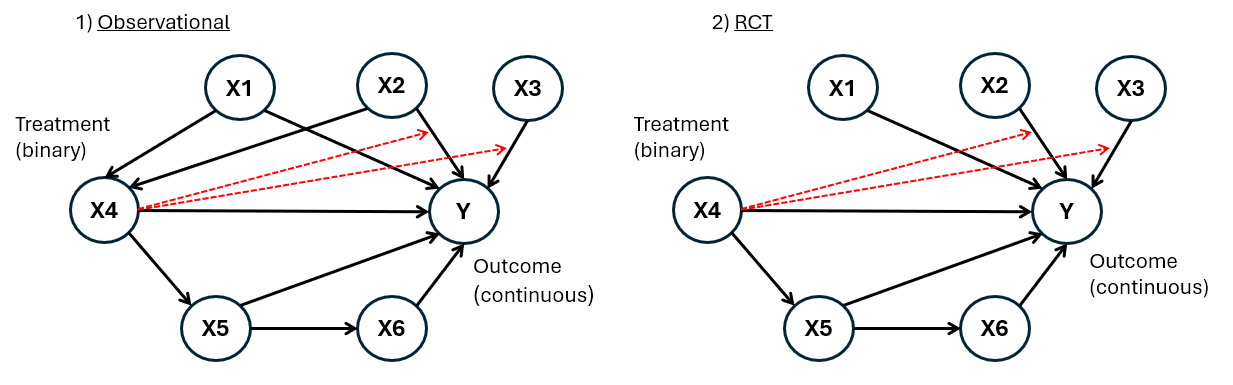
\includegraphics[width=0.85\textwidth]{img/exp4_dags.png}
\caption{DAGs used for the simulation to estimate the ITE. Left: observational; Right: RCT setting. The source nodes $X_1$, $X_2$, and $X_3$ come from a multivariate standard normal distribution ($\rho=0.1$). In the observational setting, the binary treatment $X_4$ depends on the parents $X_1$ and $X_2$. In the RCT setting, this dependency is omitted due to randomization. The outcome $Y$ depends on all variables, with additional interaction effects between the treatment and the variables $X_2$ and $X_3$. All variables except the treatment $X_4$ are continuous.}
\label{fig:ite_dag_observational}
\end{figure}

\medskip

\textbf{Illustrative scenario:} An possible real-world scenario that follows the structure of the proposed DAG could be the following: A marketing campaign is conducted to increase customer spending. The treatment is the marketing email ($X_4$) sent to customers. If the treatment is not randomized, it depends on prior total spend ($X_1$) and the customer engagement score ($X_2$). The outcome is the total spend in the 30 days following the email, denoted as $Y$. The past total spend ($X_1$) and customer engagement score ($X_2$) act as confounders, influencing both the treatment and the outcome. The customer satisfaction score ($X_3$), obtained from a recent survey, is another predictor. The time spent on the website after receiving the email ($X_5$) is a mediator that affects the number of product pages viewed ($X_6$), which in turn influences the total spend ($Y$). Interaction effects exist between the treatment ($X_4$) and both $X_2$ and $X_3$, meaning the treatment effect differs based on the customer's engagement and satisfaction levels. The goal is to estimate the individualized treatment effect (ITE) of the marketing email ($X_4$) on the total spend ($Y$), in order to personalize customer targeting.

\medskip

\section{Setup} \label{sec:methods_experiment4}

\textbf{Data-generating process:} The standard logistic distribution was chosen as the noise distribution to align with other examples in this thesis. Any other noise distribution could also be used here, as we are not interested in coefficient interpretability in this experiment. All variables except the binary treatment $X_4$ are continuous. The source nodes $X_1$, $X_2$, and $X_3$ are generated from a multivariate standard normal distribution with a compound symmetric covariance matrix ($\rho = 0.1$). These variables represent baseline patient characteristics.

In the observational setting, $X_1$ and $X_2$ act as confounders by influencing both the treatment assignment $X_4$ and the outcome $Y$. In the RCT setting, these dependencies are removed due to randomization. The mediator $X_5$ depends on treatment $X_4$, and $X_6$ depends on $X_5$. The log-odds of the continuous outcome $Y$ depend linearly on all covariates, including additional interaction terms between the treatment and $X_2$ and $X_3$. Equation~\ref{eq:outcome_dgp} defines the outcome on the log-odds scale:

\begin{equation}
h(y \mid \mathbf{X}) = h_I(y) + \boldsymbol{\beta}_X^\top \mathbf{X} + X_4 \cdot (\boldsymbol{\beta}_{TX}^\top \mathbf{X}_{\text{TX}})
\label{eq:outcome_dgp}
\end{equation}

Here, $h_I(y)$ is the intercept function, $\mathbf{X}$ is the full covariate vector, and $\mathbf{X}_{\text{TX}} = \{X_2, X_3\}$ denotes the interaction covariates that affect the outcome only when treatment is applied ($X_4 = 1$). The intercept function $h_I(y)$ must be smooth and monotonically increasing. We define it as $h_I(y) = \tan(y/2) / 0.2$ for $y \in [-2, 2]$, and extrapolate linearly at the boundaries.

The coefficients are set as $\boldsymbol{\beta}_X = (-0.5,\ 0.5,\ 0.2,\ 1.5,\ -0.6,\ 0.4)$, where the value $1.5$ represents the direct effect of treatment $X_4$ on the outcome. The interaction coefficients are set to $\boldsymbol{\beta}_{TX} = (-0.9,\ 0.7)$.

\medskip

\textbf{Three scenarios:} The experiment is conducted under three different scenarios regarding the effect of the treatment on the outcome $Y$ in the DGP: (1) both direct and interaction effects, (2) only a direct effect, and (3) only interaction effects. Depending on the scenario, the corresponding coefficients in $\boldsymbol{\beta}_X$ and $\boldsymbol{\beta}_{TX}$ are set to zero.

\medskip


\textbf{TRAM-DAG estimation:} In both the observational and RCT settings, the TRAM-DAG is fitted as an S-learner (i.e., a single model including the treatment variable). To allow for full flexibility, all nodes with parents are modeled using complex intercepts with three hidden layers of size (10, 10, 10), without batch normalization or dropout, unsing ReLU activation. This architecture enables the model to learn nonlinearities and interactions between the treatment and covariates, allowing it to estimate both potential outcomes. The model is trained on a dataset of 20,000 samples. To prevent overfitting, an additional validation set of 10,000 samples is used, and the final model is selected using early stopping based on validation loss.

\medskip

\textbf{ITE estimation procedure:} In contrast to most of the research we analyzed, where ITEs are typically defined in terms of expected values of potential outcomes, we estimate the quantile treatment effect (QTE), specifically at the median. For each individual, we calculate the difference between the medians of the potential outcome distributions under treatment and control. \citet{chernozhukov2005}, for example, highlighted the ability of quantile regression models in heterogeneous treatment effect estimation. QTEs are particularly relevant when the distributional behavior of outcomes beyond the mean is of interest. The median QTE is defined as

\begin{equation}
\text{QTE}^{(0.5)}(\mathbf{x}) = Q_{Y(1) \mid \mathbf{X} = \mathbf{x}}(0.5) - Q_{Y(0) \mid \mathbf{X} = \mathbf{x}}(0.5),
\label{eq:qte}
\end{equation}


where $Q_{Y(t) \mid \mathbf{X} = \mathbf{x}}(q)$ denotes the $q$-th quantile of the potential outcome distribution under treatment $t$.

Once the TRAM-DAG model is fitted on observed data, we can access the inverse transformation functions $X_i = h^{-1}(Z_i \mid \text{pa}(X_i))$, which represent the structural equations of the DAG. ITE estimation proceeds in three steps, according to Algorithm~\ref{alg:ite_qte}. First, the latent values $z_{ij}$ for the explanatory variables $X_i \in \{X_1, X_2, X_3, X_5, X_6\}$ are computed for each sample $j$ using the transformation functions conditioned on their observed parents. Second, the treatment variable $X_4$ is intervened on using the do-operator for both $X_4 = 0$ and $X_4 = 1$. For each of these two treatment states, $X_5$, $X_6$, and the potential outcome (distribution) $Y$ are sampled sequentially using the latent encodings and inverse transformations. This means that the counterfactuals for $X_5$ and $X_6$ are determined. This results in two potential outcome distributions per individual, as illustrated in Figure~\ref{fig:exp4_potential_outcomes}. Finally, for each individual, the median is determined for both potential outcome distributions and the QTE is calculated as the difference between the two medians. Note that estimating the potential outcomes in terms of expected values would also be possible -- either by repeatedly sampling from each outcome distribution or, potentially, by numerical integration. However, for this experiment, we chose to estimate the QTE. For simplicity, we will refer to these as ITEs throughout the remainder of the experiment.


\begin{figure}[H]
\centering
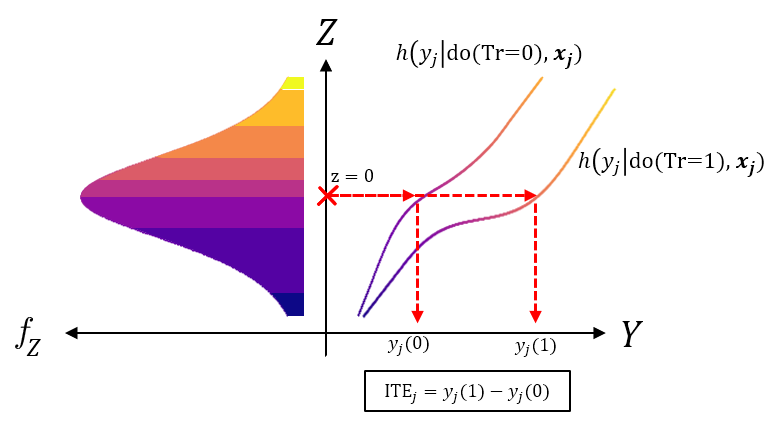
\includegraphics[width=0.6\textwidth]{img/potential_outcomes_y.png}
\caption{ITE estimation in terms of quantile treatment effect (QTE) at the median with TRAM-DAGs. The two transformation functions represent the distributions of the potential outcomes under both treatments. For the QTE(0.5), the median of the latent distribution (0 for the standard logistic) is evaluated on both transformation functions to determine the median potential outcomes. We define the ITE for an individual as the difference of the median potential outcomes.}
\label{fig:exp4_potential_outcomes}
\end{figure}


\begin{algorithm}
\caption{ITE estimation (QTE) using TRAM-DAGs}
\label{alg:ite_qte}
\begin{algorithmic}
\State \textbf{Input:} Fitted TRAM-DAG, dataset of $n$ individuals
\For{each individual $j = 1$ to $n$}
  \State \textbf{Step 1: Determine latent values}
  \For{each explanatory node $X_i \in \{X_1, X_2, X_3, X_5, X_6\}$}
    \State Compute latent value: $z_{ij} = h_i(x_{ij} \mid \text{pa}(x_{ij}))$
  \EndFor

  \State \textbf{Step 2: Generate potential outcomes under treatment and control}
  \For{$x_4 \in \{0, 1\}$} \Comment{Simulate both treatment states}
    \State Fix $X_4 = x_4$ (intervention)
    \State Sample $X_5$ and $X_6$ sequentially using $z_{ij}$ and inverse transformations
    \State Sample potential outcome $y_j(x_4)$ using $z_{7,j} = 0$ (median of the potential outcome distribution)

  \EndFor

  \State \textbf{Step 3: Compute ITE (QTE) for individual $j$}
  \State $\text{ITE}_j = y_j(1) - y_j(0)$  %\text{median}(y_j(1)) - \text{median}(y_j(0))$
\EndFor
\State \textbf{Output:} ITE estimates $\{\text{ITE}_j\}_{j=1}^n$
\end{algorithmic}
\end{algorithm}


\medskip

\textbf{Model evaluation:} Validation is conducted on the training dataset and on an independent test dataset of same size. During the data-generating process, the true potential outcomes under both treatment states were recorded for each individual, which allows for exact computation of the true ITE. The estimated ITEs are evaluated against the true values using several visual and numerical metrics. These include density plots of the estimated ITEs, scatter plots of true vs. estimated ITEs, and ITE-ATE plots where the observed ATE per ITE subgroup is computed as the difference in medians. In addition, the average of the estimated ITEs is compared to the true average ITE and to the empirical ATE from the RCT setting. The scatter plot of true versus estimated ITEs is the most informative validation, as it directly reflects how accurately the model estimated ITEs.














% 
% \textbf{ITE estimation procedure: } In contrast to the potential outcomes framework, where the potential outcomes are defined as the expected value of the outcome under treatment, we define the potential outcomes as the median of the outcome distribution under treatment - the quantile treatment effect (QTE). For simplicity, we will further refer to the individual treatment effect as ITE even though technically, the QTE is meant. Determining the potential outcomes in terms of the expected values would also be possible, but would require us to repeatedly sample from each resulting potential outcome distribution for each individual and average the results. This was computationally too time consuming and therefore we decided to estimate the QTE instead. In the ITE estimation in the previous examples with binary outcome, this was not necessary, since the potential outcomes were defined as the probabilities of the outcome under treatment and control, hence a single number that represents the expected value.
% 
% Notes after Meeting 24.06.25: Depending on the problem, CATE in terms of expected values of potential outcomes might be more appropriate than QTE, but also QTE could be better. Depends. If we wanted the potential outcomes based on the expected values, we have two options. either sample latent values and evaluate inverse tranformation functions. from those two sample distributions calculate the means to get the expected potential outcomes. Lucas suggested that we could also use numerical integreation instead, then we would not have to sample.
% 
% In contrast to the mean-based estimands above, the quantile treatment effect (QTE) evaluates differences in the distribution of potential outcomes. For instance, the median treatment effect is defined as
% 
% \citep{chernozhukov2005} also wrote about QTE (also in the context of instrumental variables). (also says to can deal with unobserved heterogeneity.. although, probably only as extension of our approach)
% 
% \begin{equation}
% \tau^{(0.5)}(x) = Q_{Y(1) \mid X = x}(0.5) - Q_{Y(0) \mid X = x}(0.5),
% \end{equation}
% 
% where $Q_{Y(t) \mid X = x}(q)$ denotes the $q$-th quantile of the potential outcome under treatment $t$. QTEs are particularly relevant when treatment effects are not symmetrically distributed or when tail behavior is of interest. In experiment 4, Section \ref{sec:methods_experiment4} we performed a simulation study using the median for the QTE estimation.
% 
% Once the TRAM-DAG is fitted, we obtained the estimated (inverse) transformation functions $X_i = h^{-1}(Z_i \mid pa(X_i))$ that represent the equations $X_i = f(Z_i, pa(X_i))$ in the structural causal model. The process for the ITE estimation is outlined in \ref{alg:ite_qte}. It is done as follows: In a first step to estimate the ITE, we determine the latent values $z_{ij}$ in all observed samples $j$ for the explanatory nodes $i$ - X1, X2, X3, X5 and X6. The latent values are the values of the transformation functions at the observed value of the variable given the observed values of its parents $z_{ij} = h_i(x_{ij} \mid pa(x_{ij}))$. In a second step, these latent values $z_{ij}$ are used to sequentially sample from the two interventional distributions when setting the treatment X4 to either 0 or 1. For each individual, these interventions impact the mediator nodes X5 and X6 as well as the outcome Y. The source nodes X1, X2 and X3 remain equal under both treatments. The treatment X4 is the variable which we fix by the do-intervention. X5 and X6 will change according to the treatment. Finally, for each set of samples $j$ (meaning for each individual) we get two distributions for the outcome, one under treatment and one under control. Then, for each individual, we calculate the iTE as the difference between the medians of the potential outcome distributions under treatment and control, as visualized in Figure~\ref{fig:exp4_potential_outcomes}.
% 
% 
% 
% 
% \begin{figure}[H]
% \centering
% 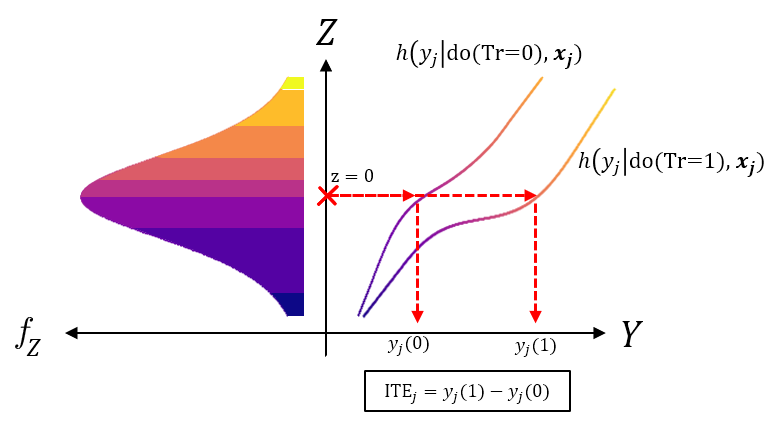
\includegraphics[width=0.6\textwidth]{img/potential_outcomes_y.png}
% \caption{Quantile treatment effect (QTE) at the median with TRAM-DAGs. The two transformation functions represent the distributions of the potential outcomes under both treatmetns. For the QTE(0.5), the median of the latent distribution is evaluated on both transformation functions to determine the median-potential-ouotcomes. This is in contrast to the ITE based on the expected values of the potential outcomes.}
% \label{fig:exp4_potential_outcomes}
% \end{figure}
% 
% 
% 
% 
% \begin{algorithm}
% \caption{ITE Estimation (QTE) Using TRAM-DAG in Observational Data}
% \label{alg:ite_qte}
% \begin{algorithmic}[1]
% \State \textbf{Input:} Fitted TRAM-DAG, observational dataset with $n$ samples
% \For{each sample $j = 1$ to $n$}
%   \State \textbf{Step 1: Encode explanatory nodes}
%   \For{each explanatory node $X_i \in \{X_1, X_2, X_3, X_5, X_6\}$}
%     \State Compute latent value: $z_{ij} = h_i(x_{ij} \mid \text{pa}(x_{ij}))$
%   \EndFor
% 
%   \State \textbf{Step 2: Generate potential outcomes under treatment and control}
%   \For{$x_4 \in \{0, 1\}$} \Comment{Simulate both treatment states}
%     \State Fix $X_4 = x_4$ (intervention)
%     \State Sample $X_5$ and $X_6$ sequentially using $z_{ij}$ and inverse transformations
%     \State Sample potential outcome $y_j^{(x_4)}$ using $z_{7,i} = 0$ (median of the potential outcome distribution)
% 
%   \EndFor
% 
%   \State \textbf{Step 3: Compute QTE for individual $j$}
%   \State $\text{ITE}_j = \text{median}(y_j^{(1)}) - \text{median}(y_j^{(0)})$
% \EndFor
% \State \textbf{Output:} ITE estimates $\{\text{ITE}_j\}_{j=1}^n$
% \end{algorithmic}
% \end{algorithm}
% 
% 
% 
% 
% 
% \textbf{Validation of results: } In the data generating mechanism, along with the actually sampled values, the potential values under both treatments are also recorded and used to determine the true QTE (the ITE based on the 50 percent quantiles of the potential outcome distributions of each individual.)
% The results are displayed by densities of the estimated ITE, the scatterplots of the true vs. estimated ITE, the ITE-ATE plot with the difference in medians as ATE within subgroups to make it comparable to the estimated ITEs. Furthermore the average of all estimated and true (dgp) ITEs are presented in table format. We further calculate the ATE as the overall difference in medians in the RCT setting and compare it to the estimated values based on the ITEs, althogh if this comparison in terms of the mean of a difference in medians is valid we did not further proof. It should be rather regarded as information, but not as proof. The scatterplot of the true vs. estimated ITE poses the most important validation.


% Check if true? probably not entirely... in both, the RCT and in the Observational setting, also other models could be applied instead of TRAM-DAG. As long as all confounders are included in the model, we controll for the confounders and can get unbiased results. For example a T-learner Colr($Y \sim X_1 + X_2 + X_3$) (because Colr is basically what we did in the DGP) fitted on both treatment groups separately could be used to estimate the ITE in our proposed experiment. This might only be possible so easily as long as we do not assume additional interactions between the treatment and the mediators $X_5$ and $X_6$. If we would assume such interactions, we would have to include these in the model as well, which would make it more complex and possibliy requires to fit and apply multiple models. If there are no interactions with the mediators, they can be omitted, since we are interested in the total treatment effects and not in separating the effect (mediation analysis). But again, we can only omit if these variables do not contain additional information about treatment effect heterogeneity. The reasoning is because to estimate the total effect one should not control for mediators. (check if really true!!!)  However, the TRAM-DAG framework is well suited to also deal with mediators and calculate counterfactuals, therefore we think it is a good example to show its capabilities.


% Notes after Meeting 24.06.25: Depending on the problem, CATE in terms of expected values of potential outcomes might be more appropriate than QTE, but also QTE could be better. Depends. If we wanted the potential outcomes based on the expected values, we have two options. either sample latent values and evaluate inverse tranformation functions. from those two sample distributions calculate the means to get the expected potential outcomes. Lucas suggested that we could also use numerical integreation instead, then we would not have to sample.











% \begin{table}
% 
% \caption{Comparison of confidence intervals for the mean differences across scenarios. The first row of each pair corresponds to the confidence interval from the linear model (lm), while the second row corresponds to the bootstrap method.}
% \centering
% \begin{tabular}[t]{lrr}
% \toprule
%   & Lower Bound & Upper Bound\\
% \midrule
% Scenario 1 (lm) & -0.58231 & -0.54359\\
% Scenario 1 (bootstrap) & -0.58210 & -0.54355\\
% Scenario 2 (lm) & -0.59118 & -0.55371\\
% Scenario 2 (bootstrap) & -0.59091 & -0.55405\\
% Scenario 3 (lm) & -0.06784 & -0.02799\\
% \addlinespace
% Scenario 3 (bootstrap) & -0.06784 & -0.02752\\
% \bottomrule
% \end{tabular}
% \end{table}

 


\section{Results}

First, we present the results for Scenario (1), which includes both direct and interaction effects  of treatment. Then, we show the results for Scenario (2), which has a direct effect but no interaction effects, and finally Scenario (3), which includes interaction effects but no direct treatment effect. For each scenario, we compare the results in an observational setting with confounded treatment allocation and in a randomized controlled trial (RCT) setting without confounding. We also compare the average treatment effect (ATE), which can be directly calculated in the RCT setting on observed outcomes, with the ATE derived from the estimated ITEs. All ITEs presented in this experiment are technically quantile treatment effects (QTEs), as defined in Equation~\ref{eq:qte}, based on the medians of the potential outcomes. For simplicity, we will refer to them as ITEs. The aim is to investigate how the TRAM-DAG performs in the presence or absence of direct and interaction effects of the treatment, both in confounded and in randomized settings, for the purpose of ITE estimation.

\subsection{Scenario (1): Direct and interaction effects} 


\begin{figure}[H]
\centering
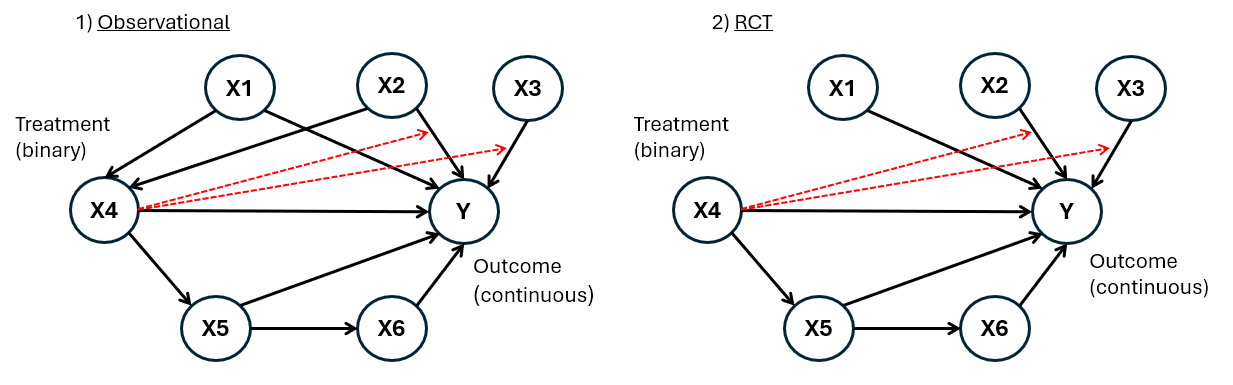
\includegraphics[width=0.85\textwidth]{img/exp4_dags.png}
\caption{DAGs for Scenario~(1), which includes a direct effect of the treatment on the outcome and additional interaction effects with covariates $X_2$ and $X_3$. These DAGs were previously shown in Figure~\ref{fig:ite_dag_observational} and is re-plotted here for convenience. Left: observational setting; Right: RCT setting.}
\label{fig:ite_dag_observational_1}
\end{figure}

Scenario~(1) includes a direct effect of the treatment on the outcome, and interaction effects with $X_2$ and $X_3$, as shown in Figure~\ref{fig:ite_dag_observational_1}. Train and test sets with 20,000 samples each were generated.

In the observational setting, treatment was confounded by $X_1$ and $X_2$. In the train set, $38.6$\% of individuals were in the control group and $61.4$\% in the treatment group. The test set had a similar distribution.

In the RCT setting, treatment was randomly assigned. In the train set, $49.8$\% were in control and $50.2$\% in treatment; in the test set, the shares were $50.2$\% and $49.8$\%, respectively.

Figure~\ref{fig:scenario1_ite_distribution_dgp} shows the true ITE distribution from the DGP, which displays some heterogeneity due to interaction effects. Figure~\ref{fig:scenario1_sampling_distributions_vertical} shows the marginal distributions of all variables in the DGP and as estimated by the TRAM-DAG. The distribution of the outcome $Y$ under $\text{do}(X_4 = 0)$ and $\text{do}(X_4 = 1)$ is shown in Figure~\ref{fig:scenario1_outcome_distributions}. The ITEs were estimated as the difference in medians of the potential outcomes. Figure~\ref{fig:scenario1_ite_densities_train_test} compares the densities of the estimated and true ITEs. In both observational and RCT settings, the estimated ITEs are close to the true ones in both train and test sets. Figure~\ref{fig:scenario1_ite_scatter_train_test} shows the scatterplots of estimated vs. true ITEs. Figures~\ref{fig:observ_scenario1_ite_ATE} and \ref{fig:rct_scenario1_ite_ATE} show the ITE-ATE plots, where the ATE is calculated as the median difference in observed outcomes within ITE subgroups. The trends are similar across train and test sets.



The ATEs calculated based on different measures in both the training and test sets are shown in Table~\ref{tab:scenario1_ate_comparison}. In the RCT setting (training set), the difference in means of the outcomes between the two treatment groups was 
$-0.563$, with a confidence interval of 
$-0.582$ to 
$-0.543$. 



% 
% Scenario (1) included a direct effect of the treatment on the outcome and an additional interaction effect of the treatment with the covariates X2 and X3, as presented in Figure~\ref{fig:ite_dag_observational_1}. A train and test set were generated with 20,000 observations each. 
% In the observational setting, the treatment allocation was confounded by the covariates X1 and X2.  In the train set, $round(observ_scenario1$dev_treatment_allocation[1]*100, 1)$\% of patients were in the control group and $round(observ_scenario1$dev_treatment_allocation[2]*100, 1)$\% were in the treatment group. This ratio was similar in the test set. 
% In the RCT setting treatment allocation was randomized. In the train set $round(rct_scenario1$dev_treatment_allocation[1]*100, 1)$\% individuals were in the control group and $round(rct_scenario1$dev_treatment_allocation[2]*100, 1)$\% in the treatment group. In the test set $round(rct_scenario1$val_treatment_allocation[1]*100, 1)$\% were in the control group and $round(rct_scenario1$val_treatment_allocation[2]*100, 1)$\% in the treatment group. 
% Figure \ref{fig:scenario1_ite_distribution_dgp} illustrates the true ITE distribution that resulted from the DGP. Due to the interaction effects, there is some heterogeneity in the ITE distribution. Figure \ref{fig:scenario1_sampling_distributions_vertical} shows the marginal distributions of all variables according to the DGP and the estimates by the fitted TRAM-DAG. Figure \ref{fig:scenario1_outcome_distributions} shows the distribution of the outcome ($Y$) under the do(Tr=0) and do(Tr=1) interventions. The fitted model was applied to estimate the ITEs in terms of the difference in medians of the potential outcomes. The resulting density of the estimated ITEs compared to the true ITEs according to the DGP is shown in Figure \ref{fig:scenario1_ite_densities_train_test}. Across both settings, the densities of the estimated ITEs are close to the true densities in both the training and test datasets. Figure \ref{fig:scenario1_ite_scatter_train_test} shows the scatterplots of true against estimated ITEs. Finally, Figure \ref{fig:scenario1_ite_cATE} displays the ITE-ATE plot where the ATE is computed as the difference in medians of the observed outcome under the treatments within the respective ITE-subgroups. The trends observed in the training and test sets are consistent.


% The average treatment effect (ATE) is presented in Table \ref{tab:scenario1_ate_comparison}. In the RCT setting in the training set, the difference in means of the outcomes in the two treatment groups was $round(rct_scenario1$dev_ATE_observed_Y_mean_diff, 3)$ with a confidence interval of $round(rct_scenario1$dev_ATE_observed_Y_mean_diff_CI[1], 3)$ to $round(rct_scenario1$dev_ATE_observed_Y_mean_diff_CI[2], 3)$. The ATEs calculated based on different measuress in the training and test dataset, are shown in Table \ref{tab:scenario1_ate_comparison}.


% The ATE in terms of the difference in medians of the observed outcomes was $round(rct_scenario1$dev_ATE_observed_Y_median_diff, 3)$. Also in the training set, the ATE in terms of the mean of the true ITEs was $round(rct_scenario1$dev_ITE_median_average, 3)$ and the ATE in terms of the mean of the estimated ITEs was $round(rct_scenario1$dev_ITE_median_pred_average, 3)$. 


\begin{table}[htbp]
\centering
\small
\caption{Scenario (1), including direct and interaction effects: Comparison of ATE measures across training and test sets for the observational and RCT settings. $\text{Y}_\text{observed}^{(\text{Tr})}$ denotes the observed outcome under the treatment ($\text{Tr}$) actually received. Estimates based on these observed outcomes (means and medians) are provided only for the RCT setting, as the observational setting is confounded. The true ITEs ($\text{ITE}_\text{true}$) were calculated for each individual based on the data-generating process. In contrast, the estimated ITEs ($\text{ITE}_\text{estimated}$) are obtained from the TRAM-DAG trained on observed data. The estimated ATE from $\text{mean}(\text{ITE}_\text{estimated})$ can be directly compared to the true $\text{mean}(\text{ITE}_\text{true})$, whereas comparisons to empirical ATEs from observed outcome differences should be interpreted with caution. All ITEs were computed based on the medians of potential outcomes under treatment and control, as defined in Equation~\ref{eq:qte}.}

\caption{Scenario (1), including direct and interaction effects: Comparison of ATE measures across training and test sets for the observational and RCT settings. $\text{Y}_\text{observed}^{(\text{Tr})}$ denotes the observed outcome under the treatment ($\text{Tr}$) actually received. Estimates based on these observed outcomes (means and medians) are provided only for the RCT setting, as the observational setting is confounded. The true ITEs ($\text{ITE}_\text{true}$) were calculated for each individual based on the data-generating process. In contrast, the estimated ITEs ($\text{ITE}_\text{estimated}$) were obtained from the TRAM-DAG trained on observed data. The estimated ATE based on $\text{mean}(\text{ITE}_\text{estimated})$ can be directly compared to the true $\text{mean}(\text{ITE}_\text{true})$, whereas comparisons to empirical ATEs from observed outcome differences should be interpreted with caution. All ITEs were computed as quantile treatment effects (QTEs) based on the median of the potential outcome distributions, as defined in Equation~\ref{eq:qte}.
}

\label{tab:scenario1_ate_comparison}
\begin{tabular}{l c c c c}
\toprule
\textbf{Measure} & \multicolumn{2}{c}{\textbf{Observational}} & \multicolumn{2}{c}{\textbf{RCT}} \\
\cmidrule(lr){2-3} \cmidrule(lr){4-5}
 & \textbf{Train} & \textbf{Test} & \textbf{Train} & \textbf{Test} \\
\midrule
ATE as $\text{mean}(\text{Y}_\text{observed}^{(1)}) - \text{mean}(\text{Y}_\text{observed}^{(0)})$ 
& NA & NA 
& -0.563 
& -0.563 \\

ATE as $\text{median}(\text{Y}_\text{observed}^{(1)}) - \text{median}(\text{Y}_\text{observed}^{(0)})$  
& NA & NA 
& -0.626 
& -0.638 \\

ATE as mean(ITE$_\text{true}$)  
& -0.620 
& -0.622 
& -0.620 
& -0.622 \\

ATE as mean(ITE$_\text{estimated}$) 
& -0.617 
& -0.620 
& -0.619 
& -0.622 \\
\bottomrule
\end{tabular}
\end{table}

% 
% \begin{table}[htbp]
% \centering
% \small
% \caption{Scenario (1), including direct and interaction effects: Comparison of ATE measures across train and test sets for the observational and RCT setting.}
% \label{tab:scenario1_ate_comparison_old}
% \begin{tabular}{l c c c c}
% \toprule
% \textbf{Measure} & \multicolumn{2}{c}{\textbf{Observational}} & \multicolumn{2}{c}{\textbf{RCT}} \\
% \cmidrule(lr){2-3} \cmidrule(lr){4-5}
%  & \textbf{Train} & \textbf{Test} & \textbf{Train} & \textbf{Test} \\
% \midrule
% ATE as $\text{mean}(\text{Y}_\text{observed}^{(1)}) - \text{mean}(\text{Y}_\text{observed}^{(0)})$ & NA & NA & round(rct_scenario1$dev_ATE_observed_Y_mean_diff, 3) & round(rct_scenario1$val_ATE_observed_Y_mean_diff, 3) \\
% ATE as $\text{median}(\text{Y}_\text{observed}^{(1)}) - \text{median}(\text{Y}_\text{observed}^{(0)})$  & NA & NA & round(rct_scenario1$dev_ATE_observed_Y_median_diff, 3) & round(rct_scenario1$val_ATE_observed_Y_median_diff, 3) \\
% ATE as mean(ITE$_\text{true}$)  & round(observ_scenario1$dev_ITE_median_average, 3) & round(observ_scenario1$val_ITE_median_average, 3) & round(rct_scenario1$dev_ITE_median_average, 3) & round(rct_scenario1$val_ITE_median_average, 3) \\
% ATE as mean(ITE$_\text{estimated}$) & round(observ_scenario1$dev_ITE_median_pred_average, 3) & round(observ_scenario1$val_ITE_median_pred_average, 3) & round(rct_scenario1$dev_ITE_median_pred_average, 3) & round(rct_scenario1$val_ITE_median_pred_average, 3) \\
% \bottomrule
% \end{tabular}
% \end{table}




\begin{figure}[htbp]
\centering
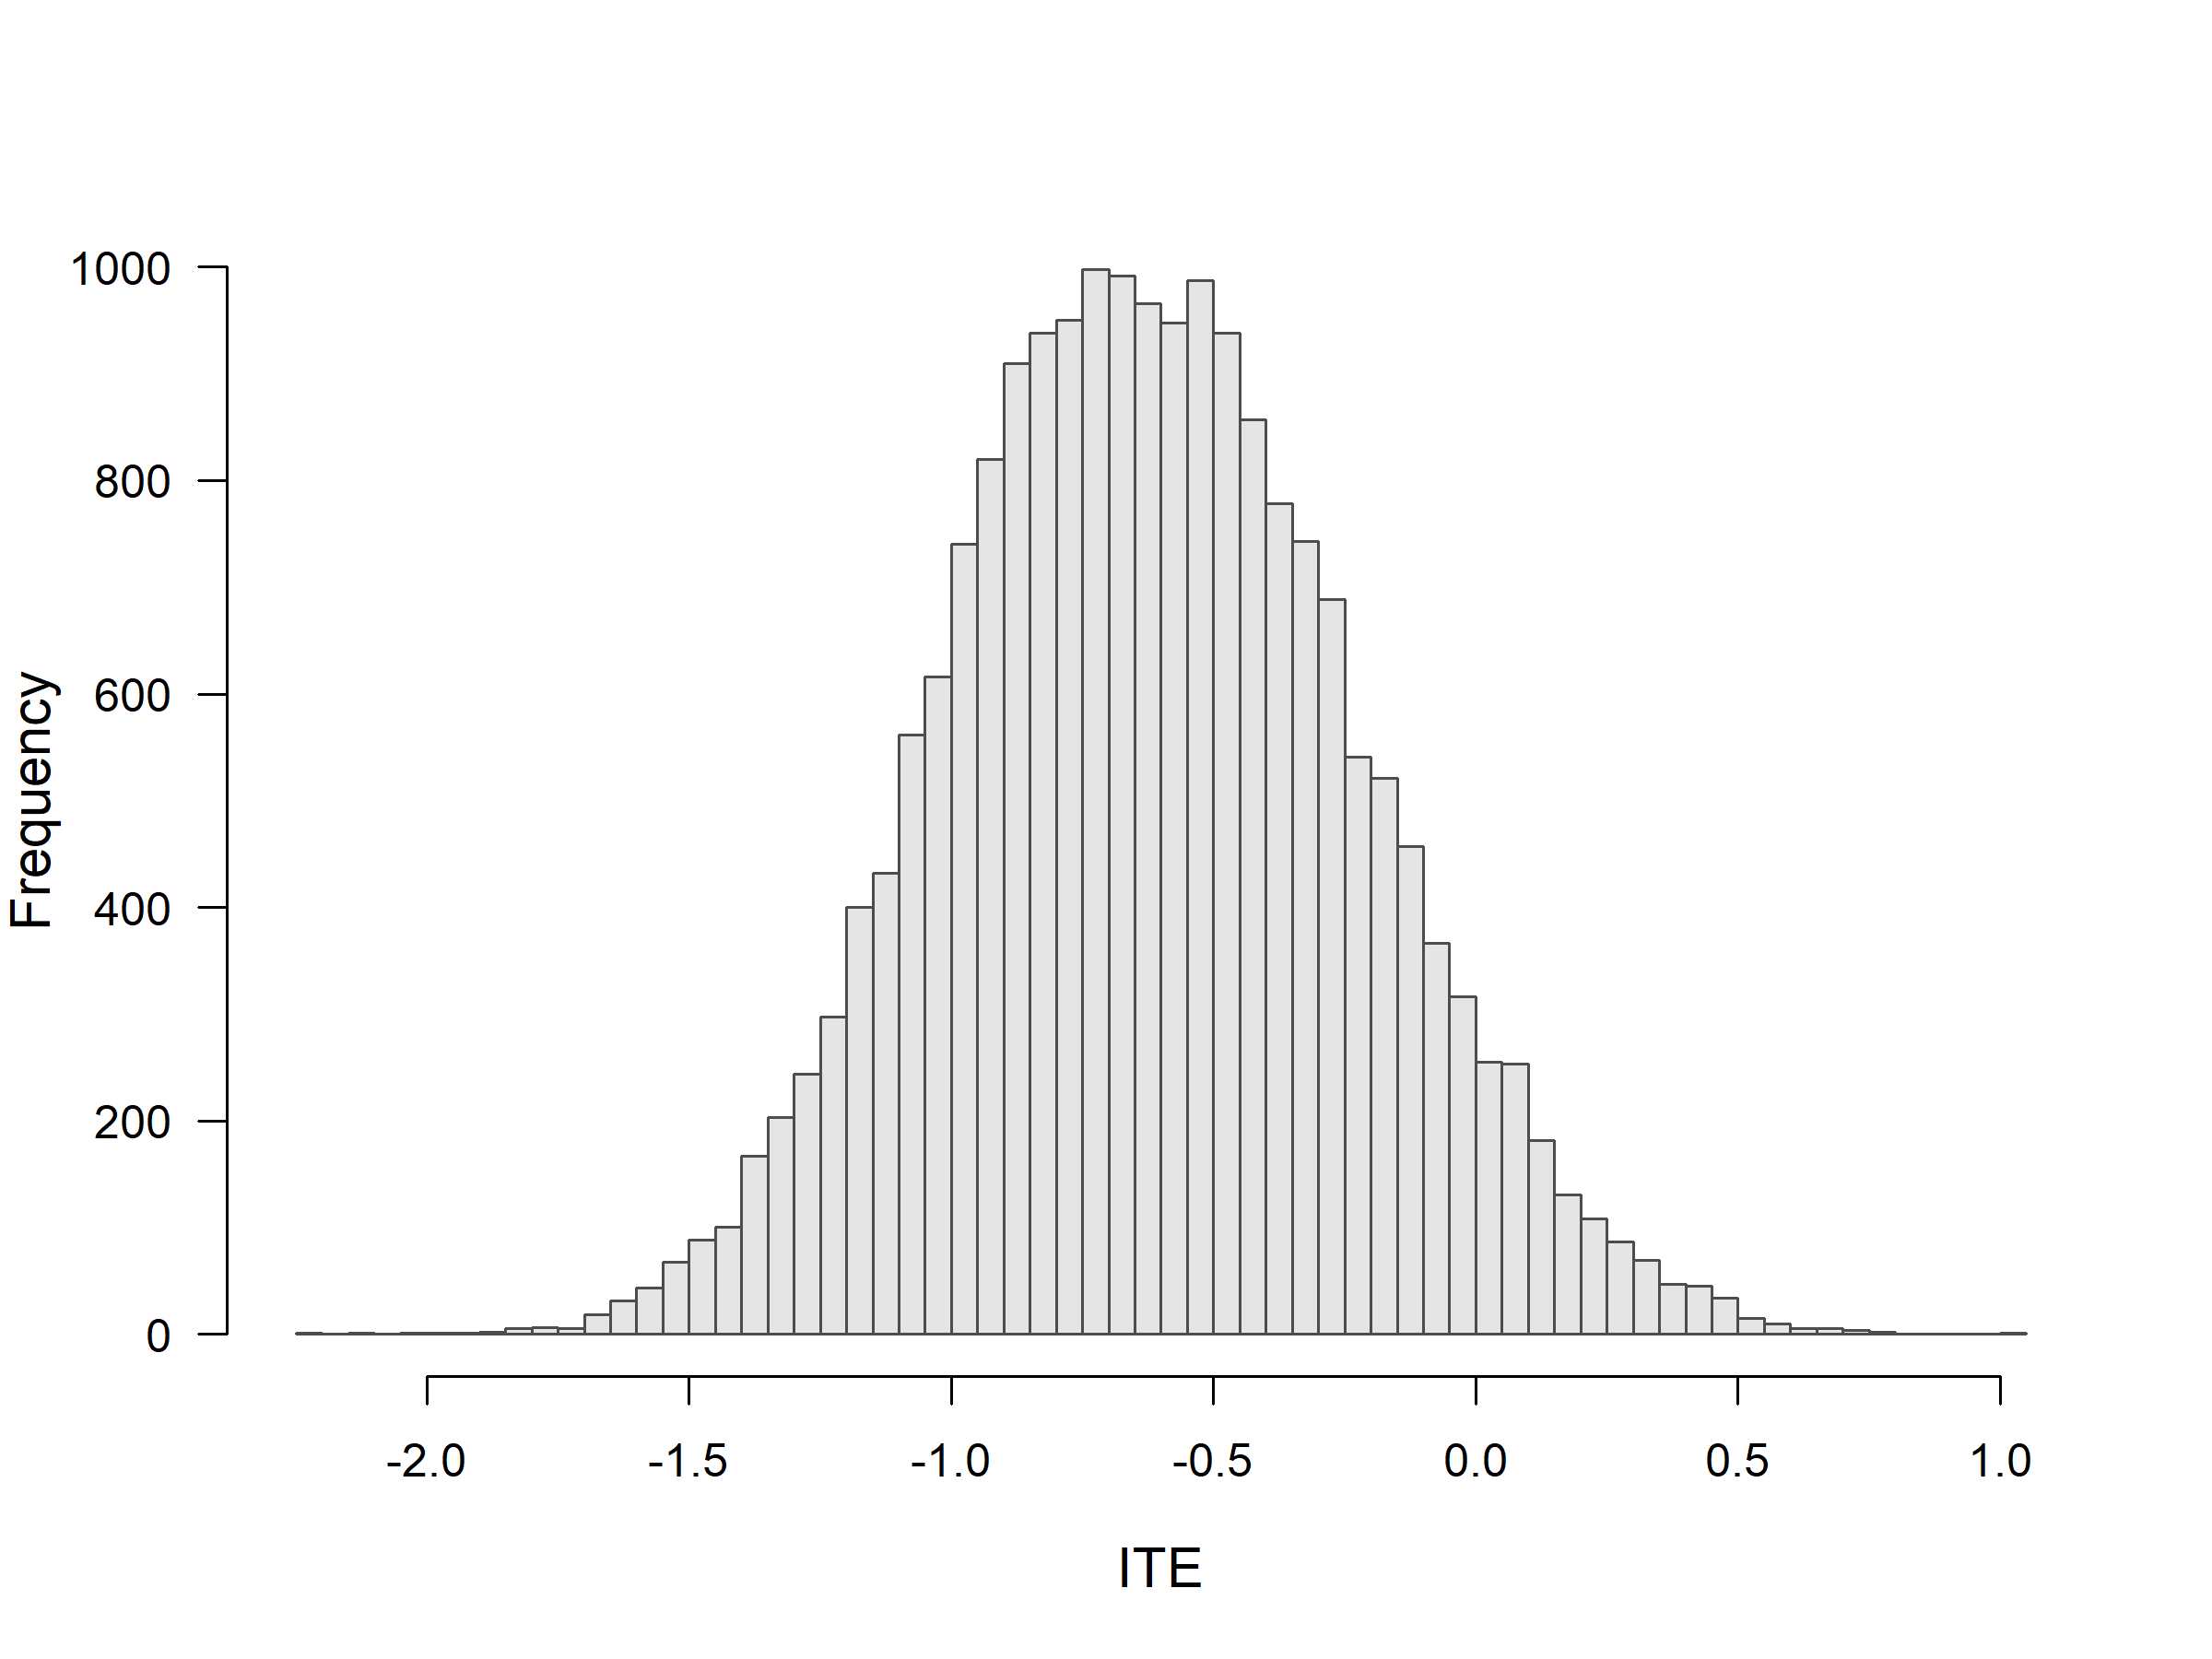
\includegraphics[width=0.7\textwidth]{img/results/observ_scenario1_ite_distribution_dgp.png}
\caption{True ITE distribution resulting from the DGP for Scenario (1), which includes both direct and interaction effects. The true ITEs are identical for each individual in the observational and RCT settings, as they are based on the potential outcomes under both treatment conditions.}
\label{fig:scenario1_ite_distribution_dgp}
\end{figure}



\begin{figure}[htbp]
\centering
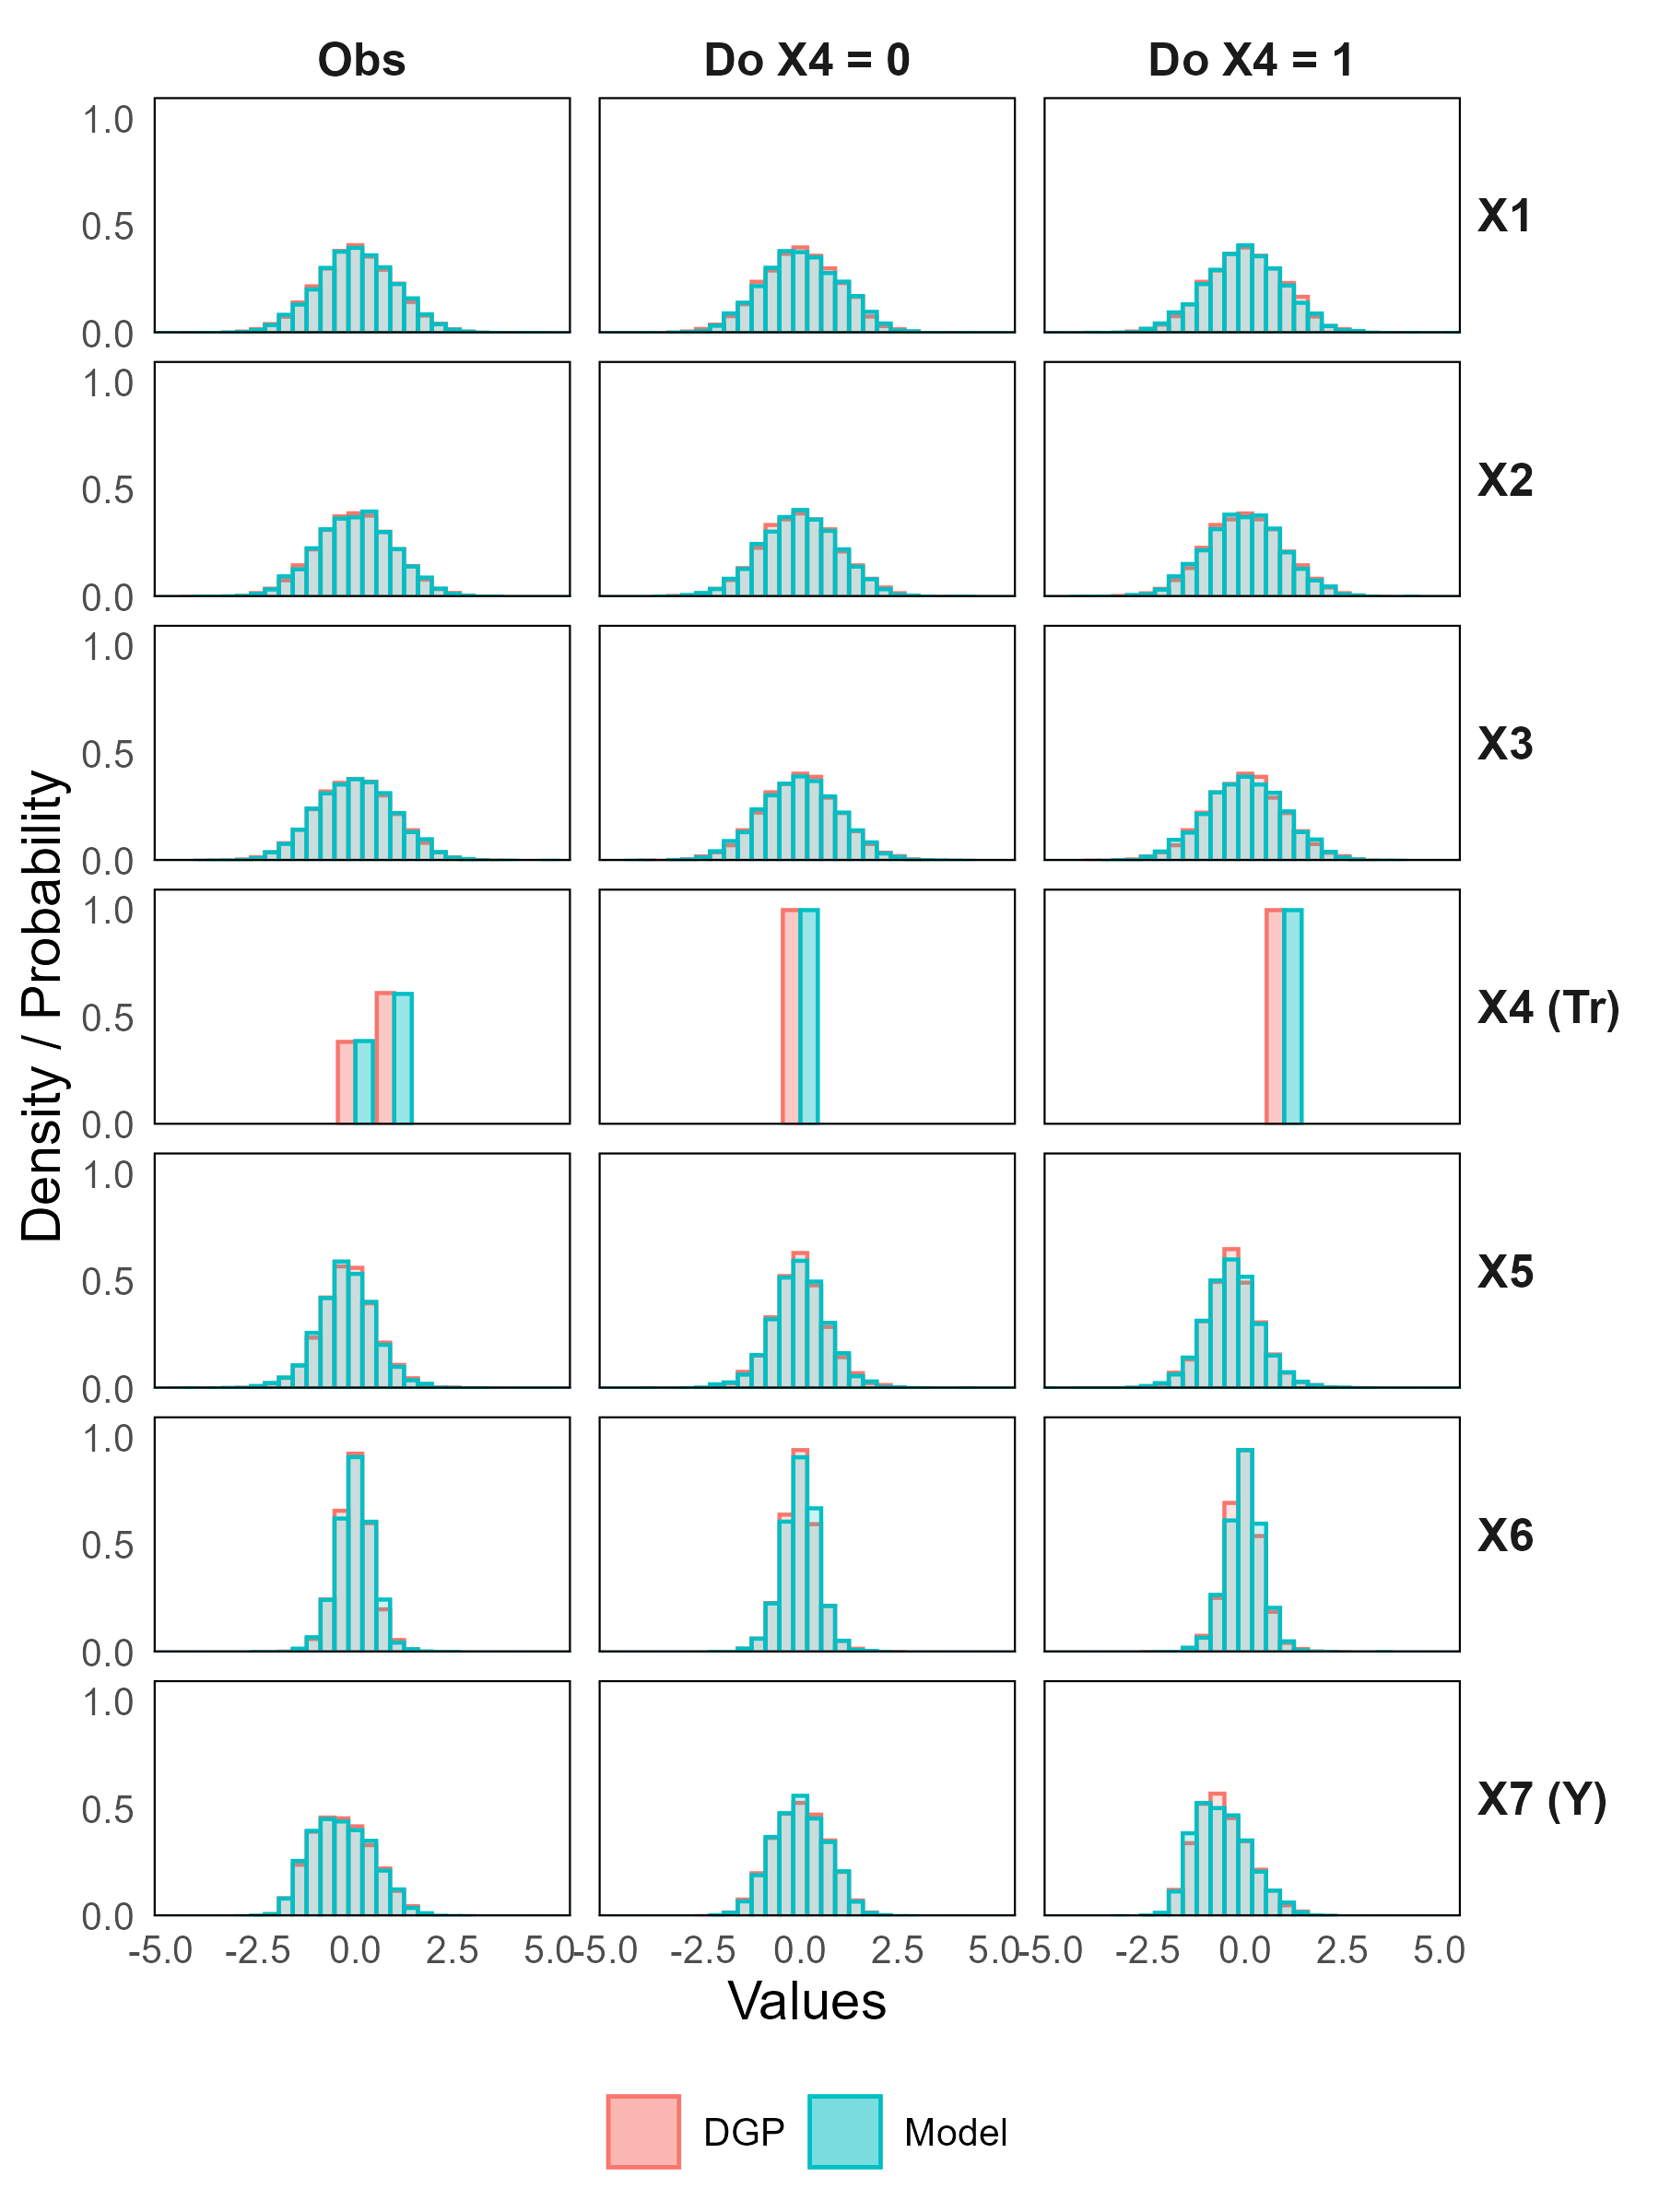
\includegraphics[width=0.45\textwidth]{img/results/observ_scenario1_sampling_distributions_vertical.png}
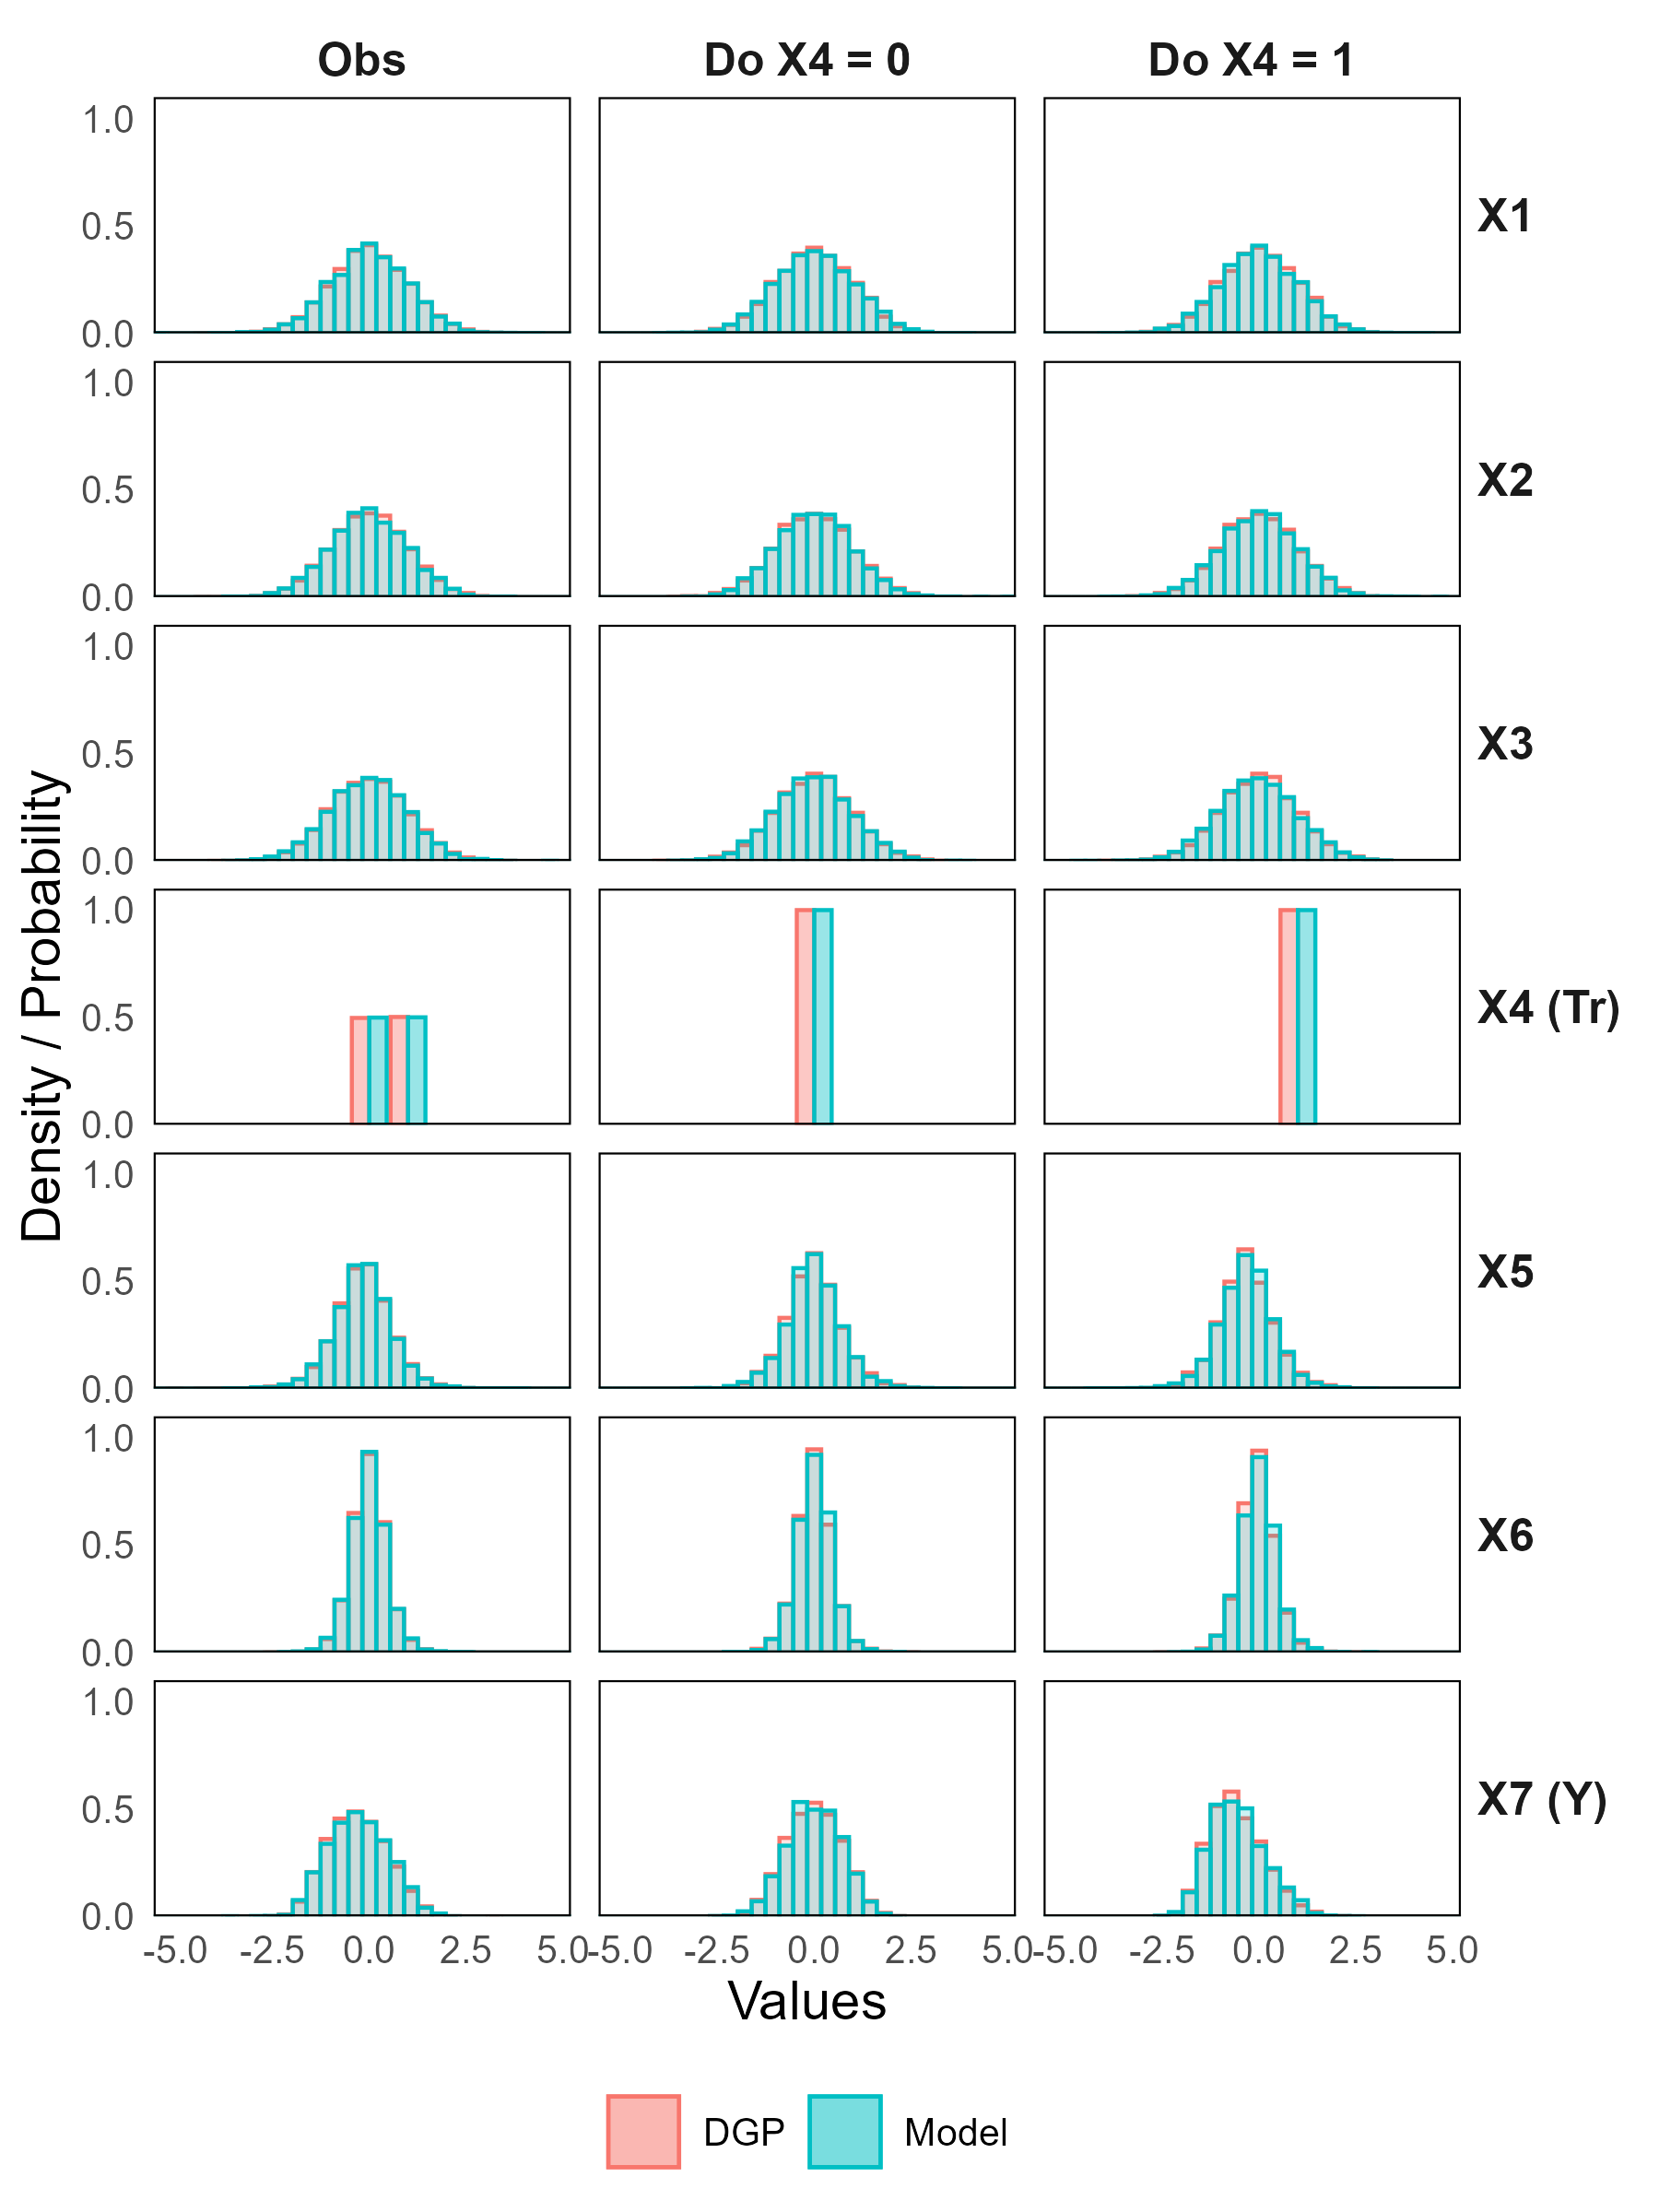
\includegraphics[width=0.45\textwidth]{img/results/rct_scenario1_sampling_distributions_vertical.png}
\caption{Marginal distributions of variables from the DGP and from samples generated by the fitted TRAM-DAG for Scenario (1) with direct and interaction effects. Distributions are shown as observed (Obs), under the control intervention (do($X_4 = 0$)), and under the treatment intervention (do($X_4 = 1$)). Left: Observational; Right: RCT setting.}
\label{fig:scenario1_sampling_distributions_vertical}
\end{figure}


\begin{figure}[htbp]
\centering
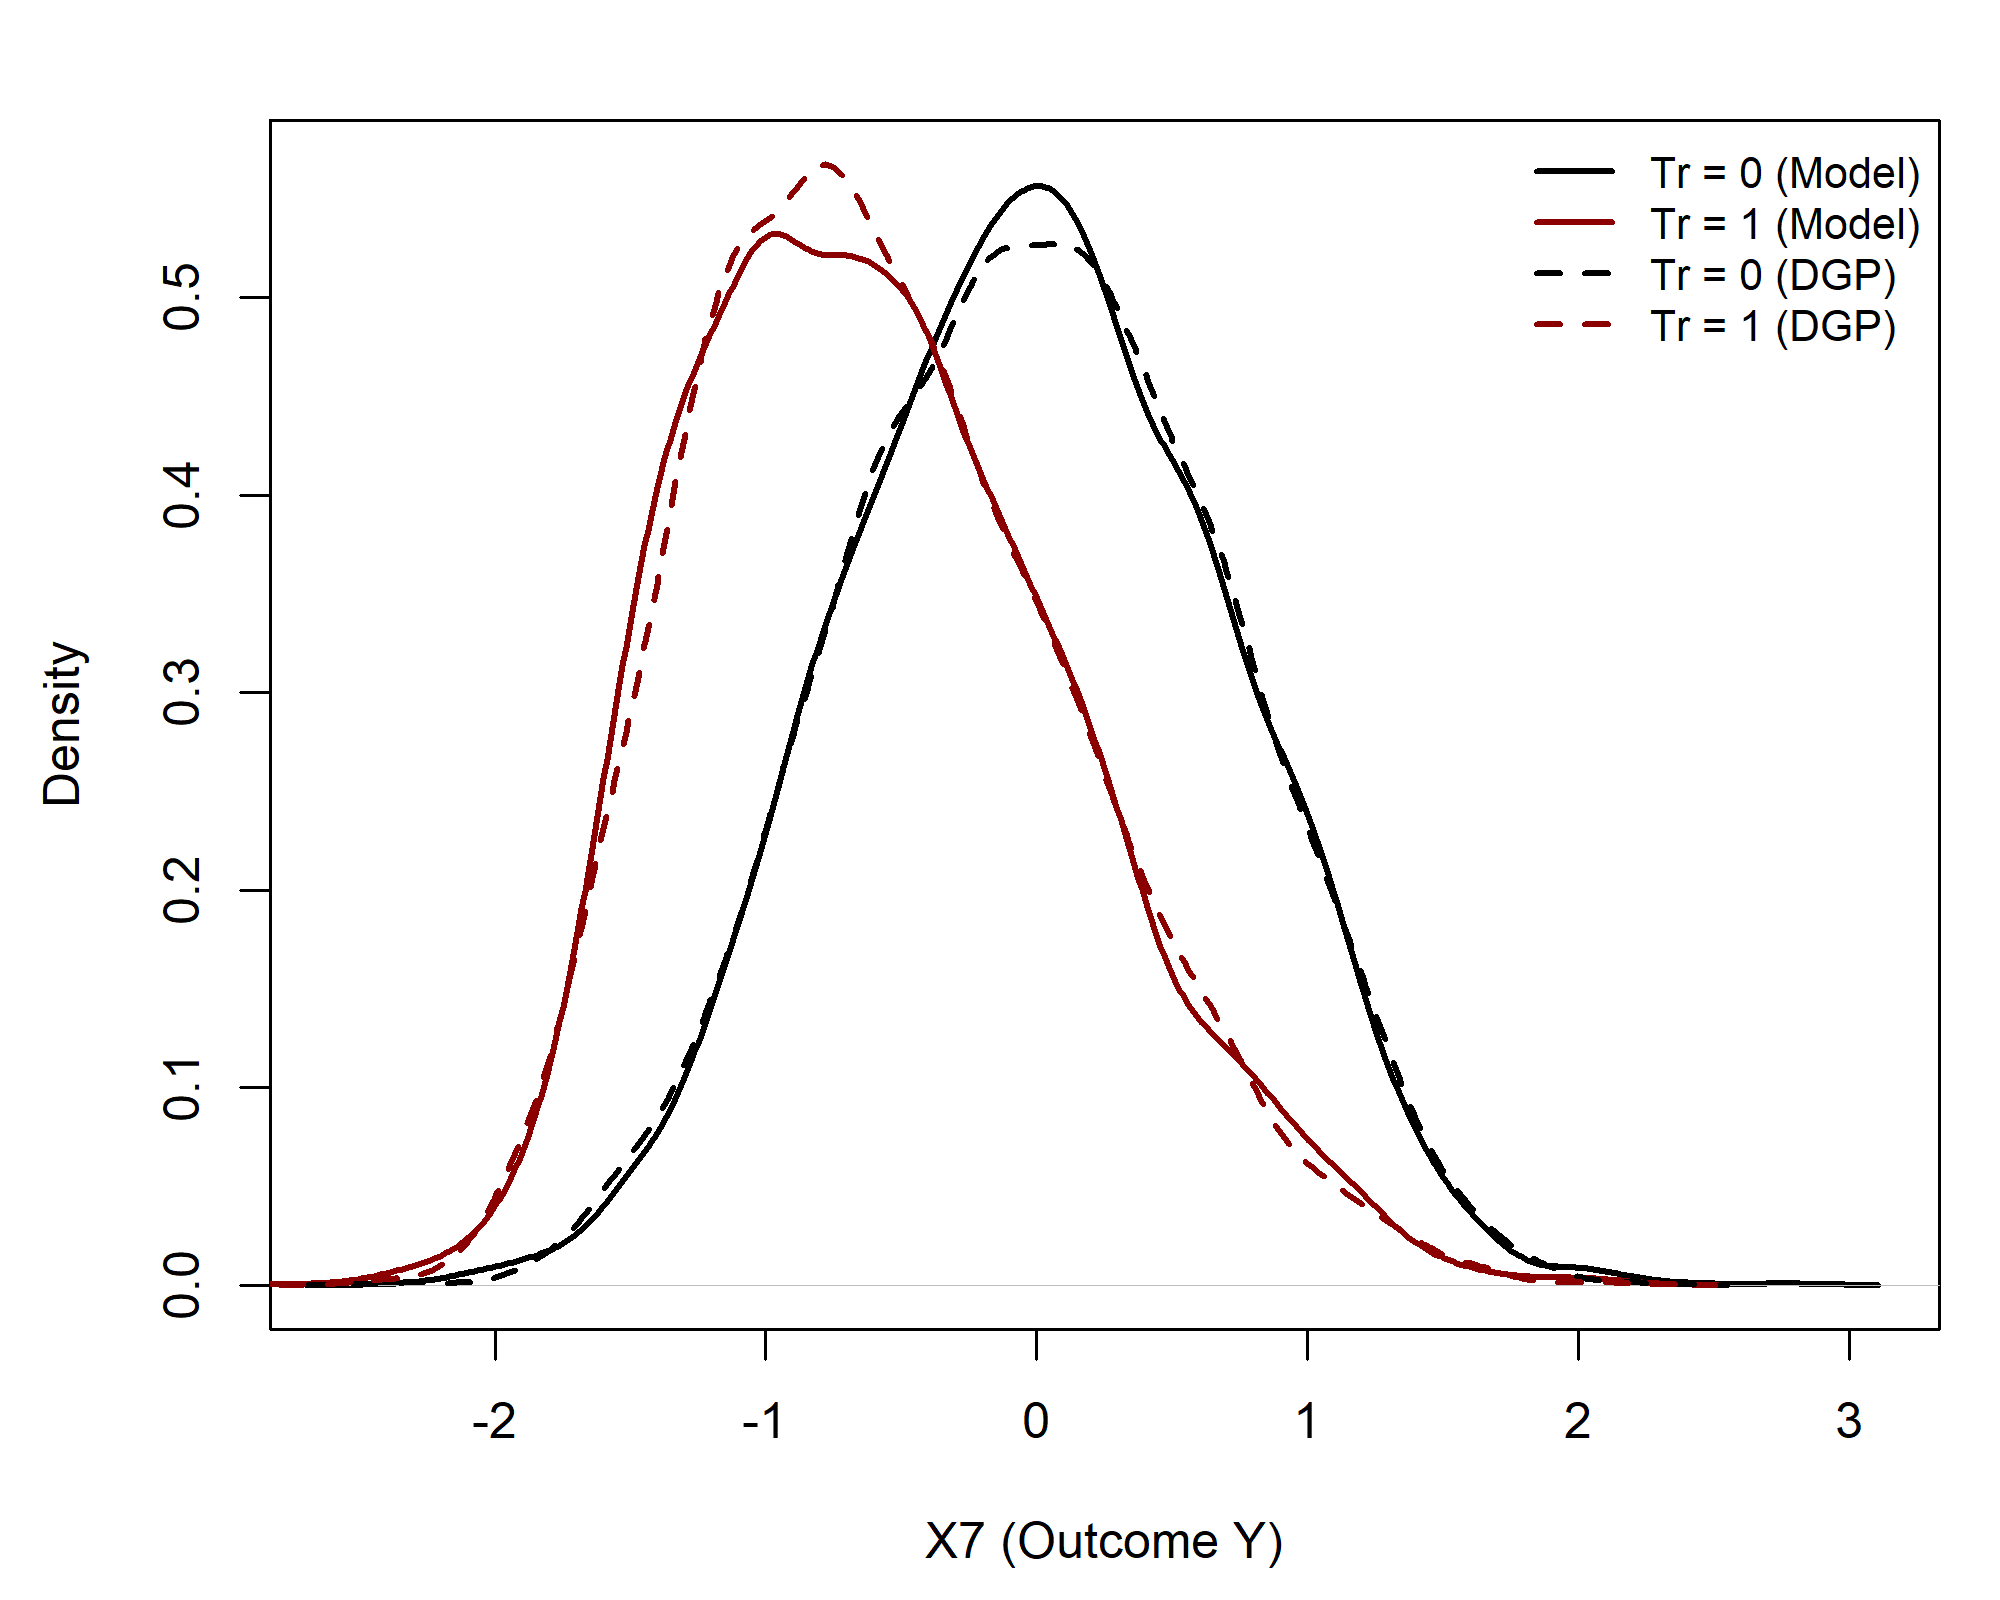
\includegraphics[width=0.45\textwidth]{img/results/observ_scenario1_X7_treatment_densities.png}
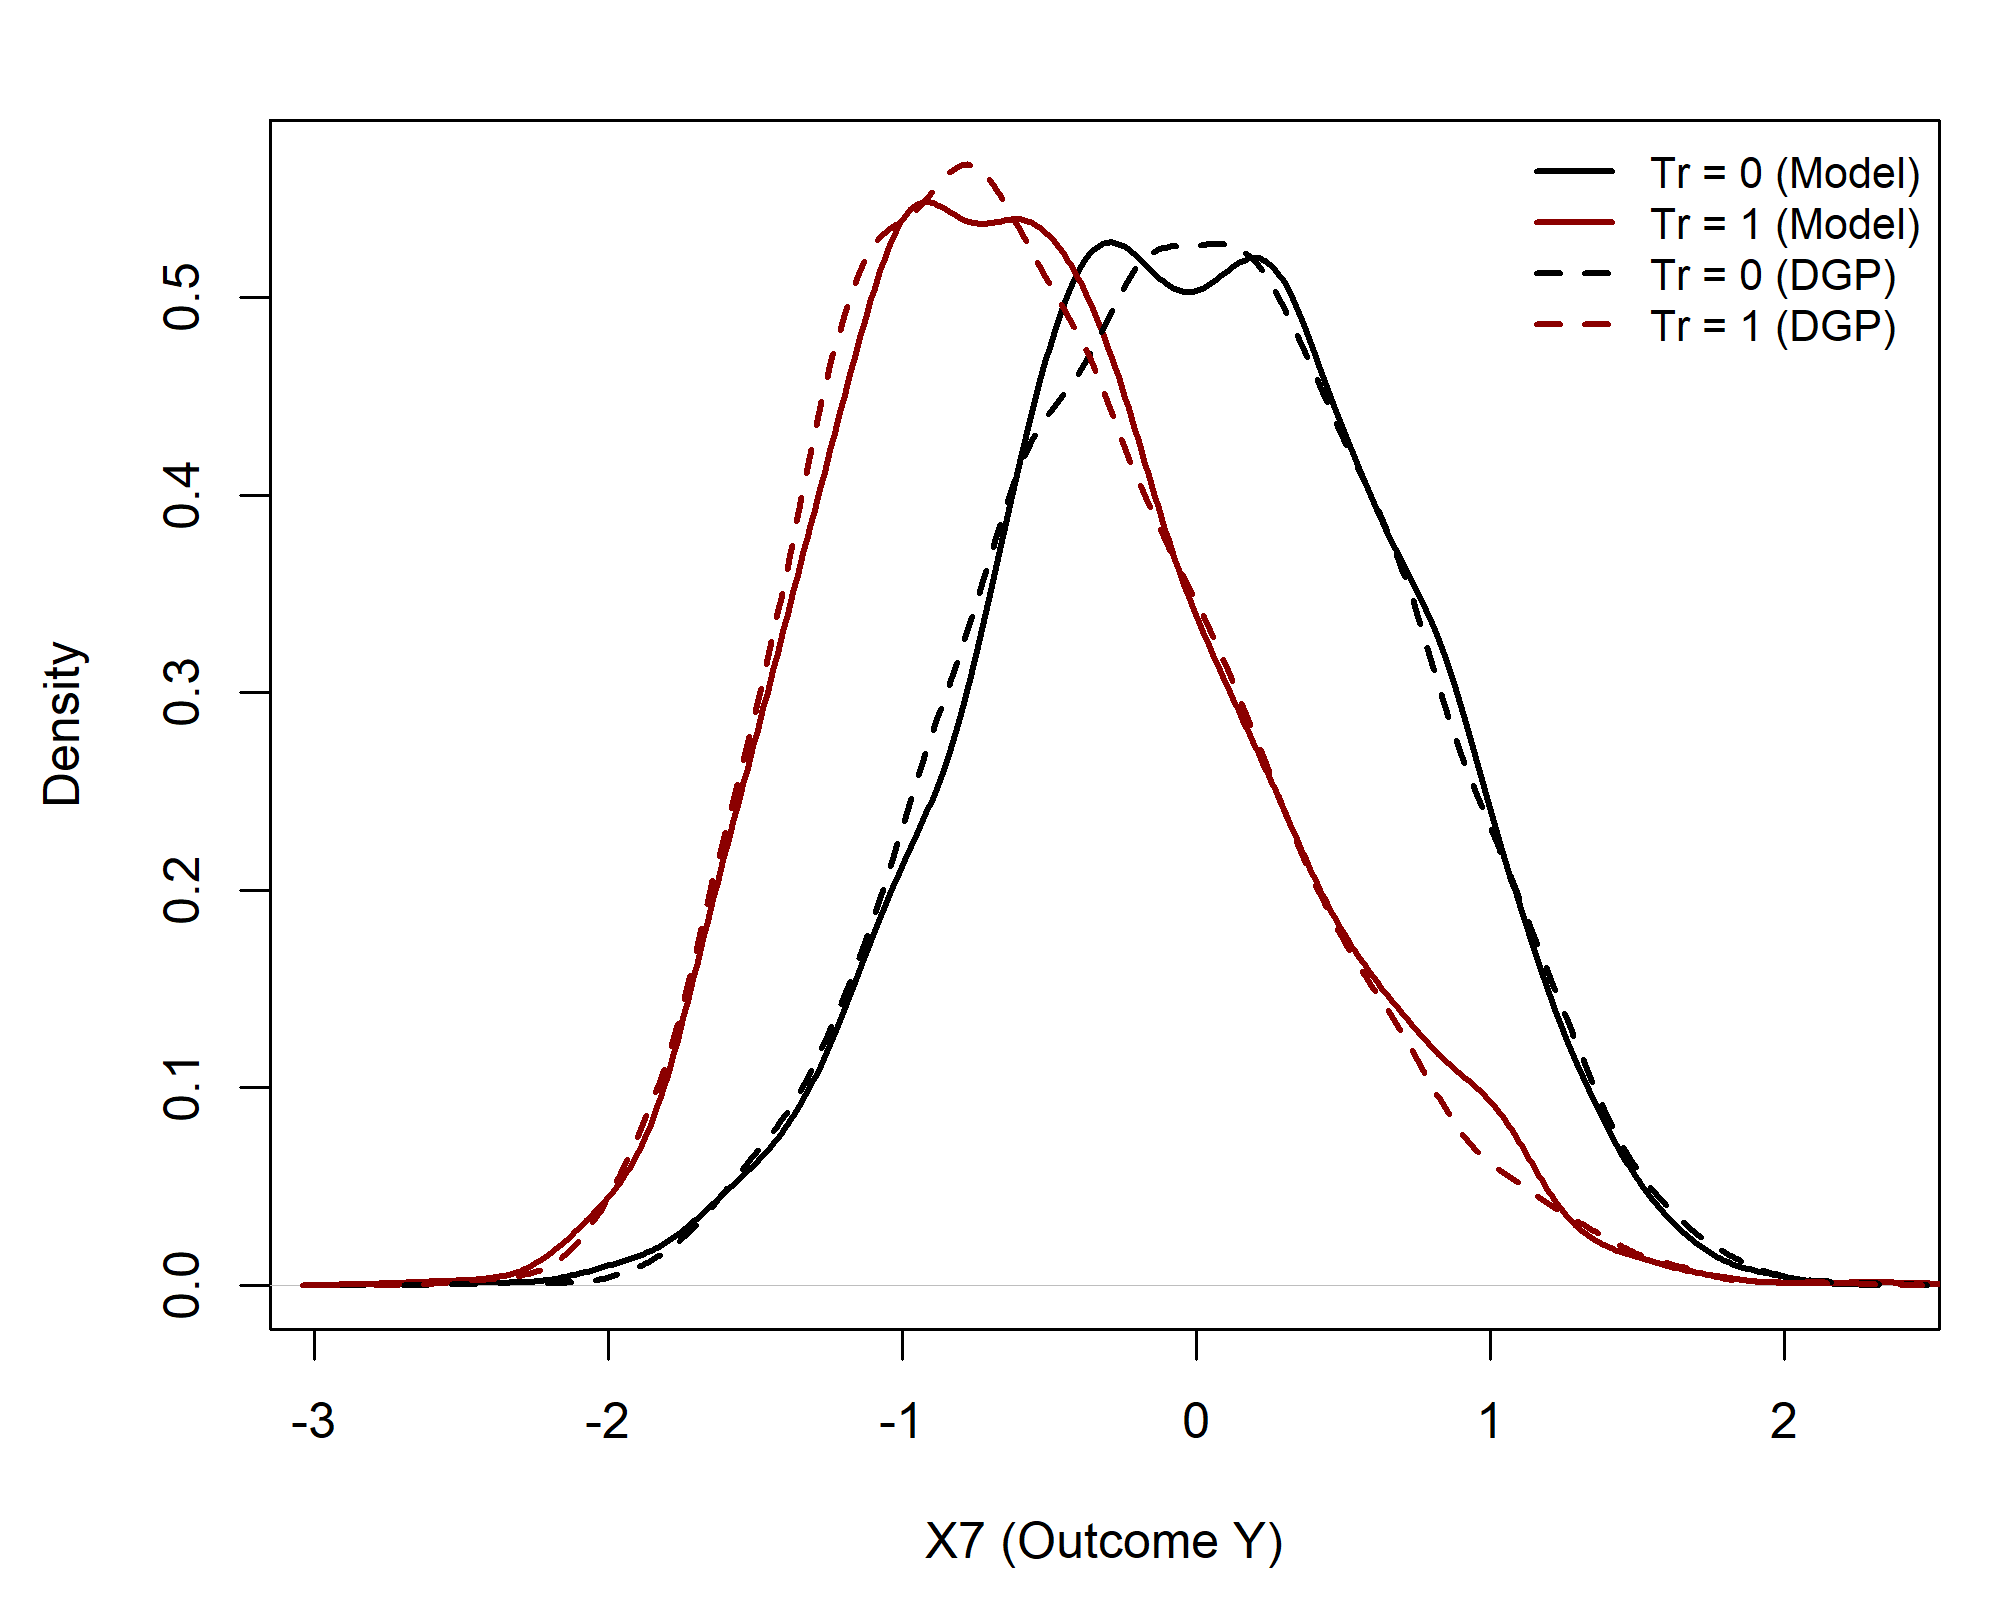
\includegraphics[width=0.45\textwidth]{img/results/rct_scenario1_X7_treatment_densities.png}
\caption{Distributions of the outcome variable ($X_7$) under control and treatment interventions for Scenario (1), which includes both direct and interaction effects. This plot provides a more detailed view of the $X_7$ panels shown under do($X_4=0$) and do($X_4=1$) in Figure~\ref{fig:scenario1_sampling_distributions_vertical}. Left: Observational; Right: RCT setting.}
\label{fig:scenario1_outcome_distributions}
\end{figure}




\begin{figure}[htbp]
\centering
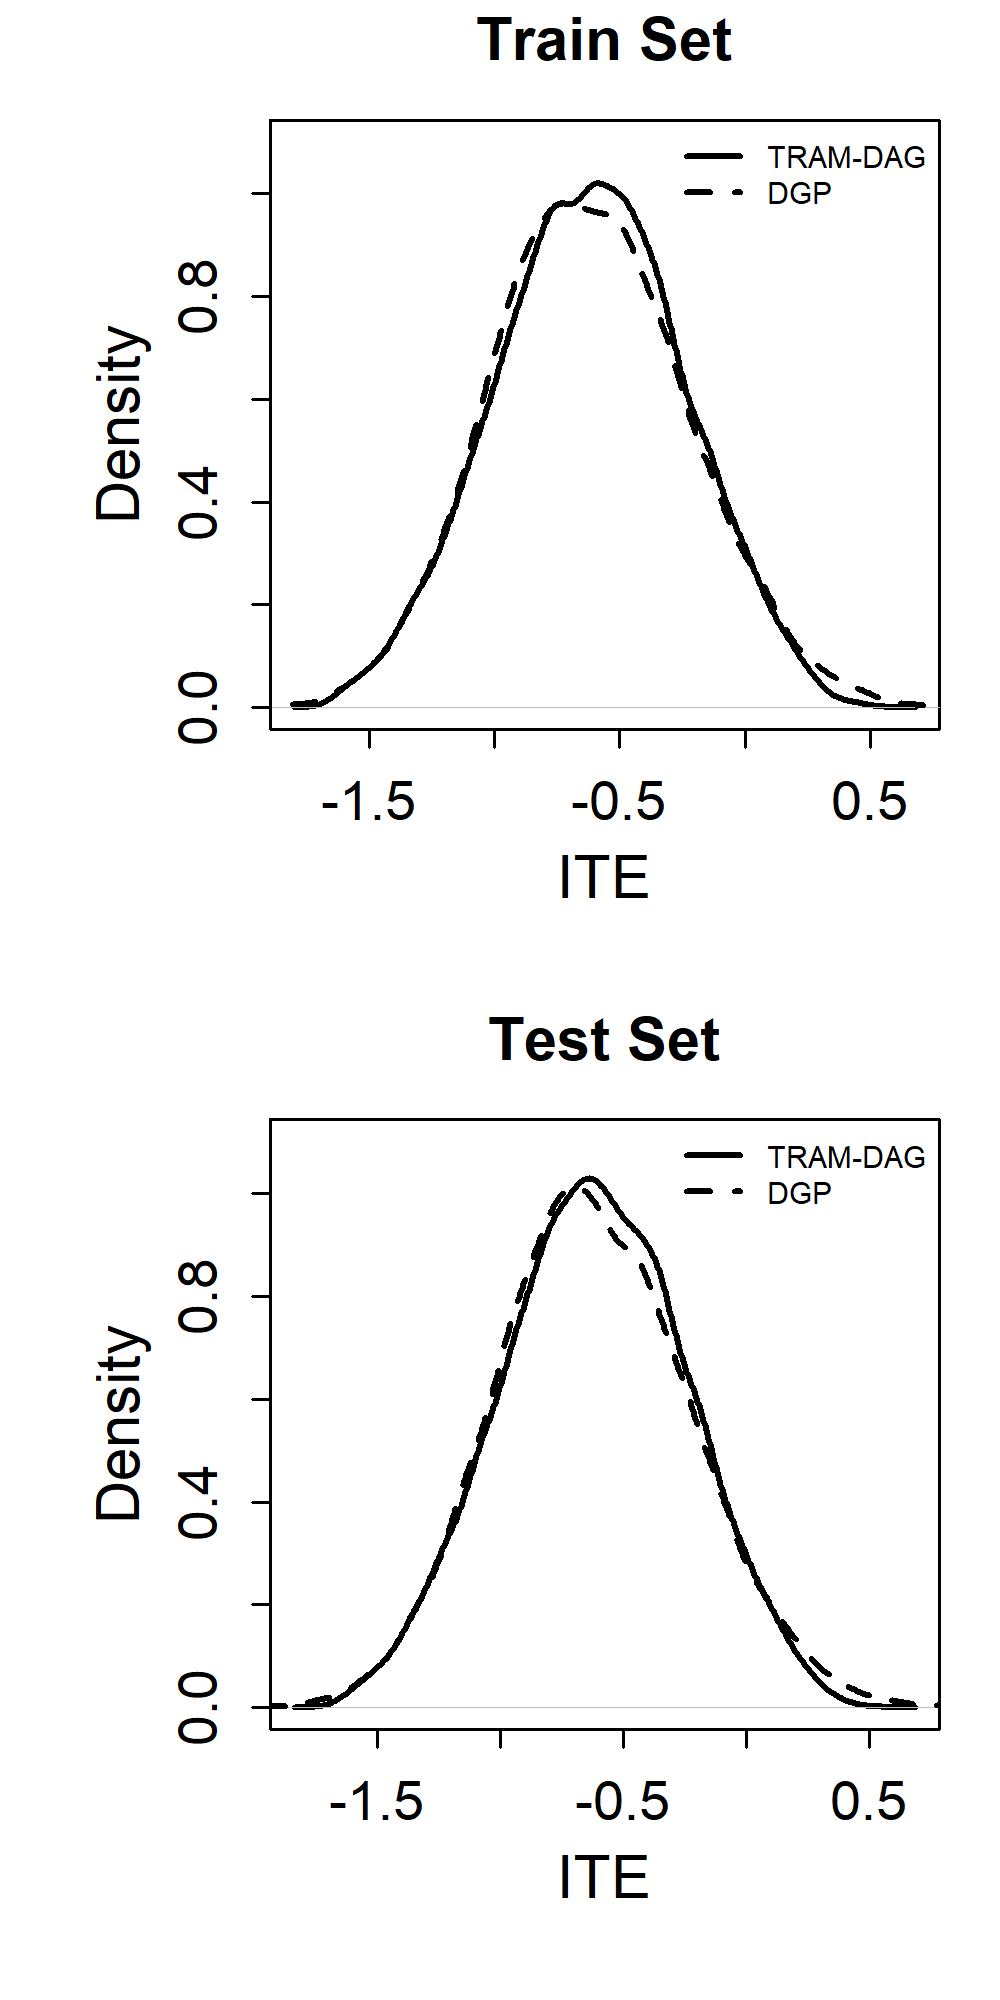
\includegraphics[width=0.33\textwidth]{img/results/observ_scenario1_ITE_densities_train_test.png} 
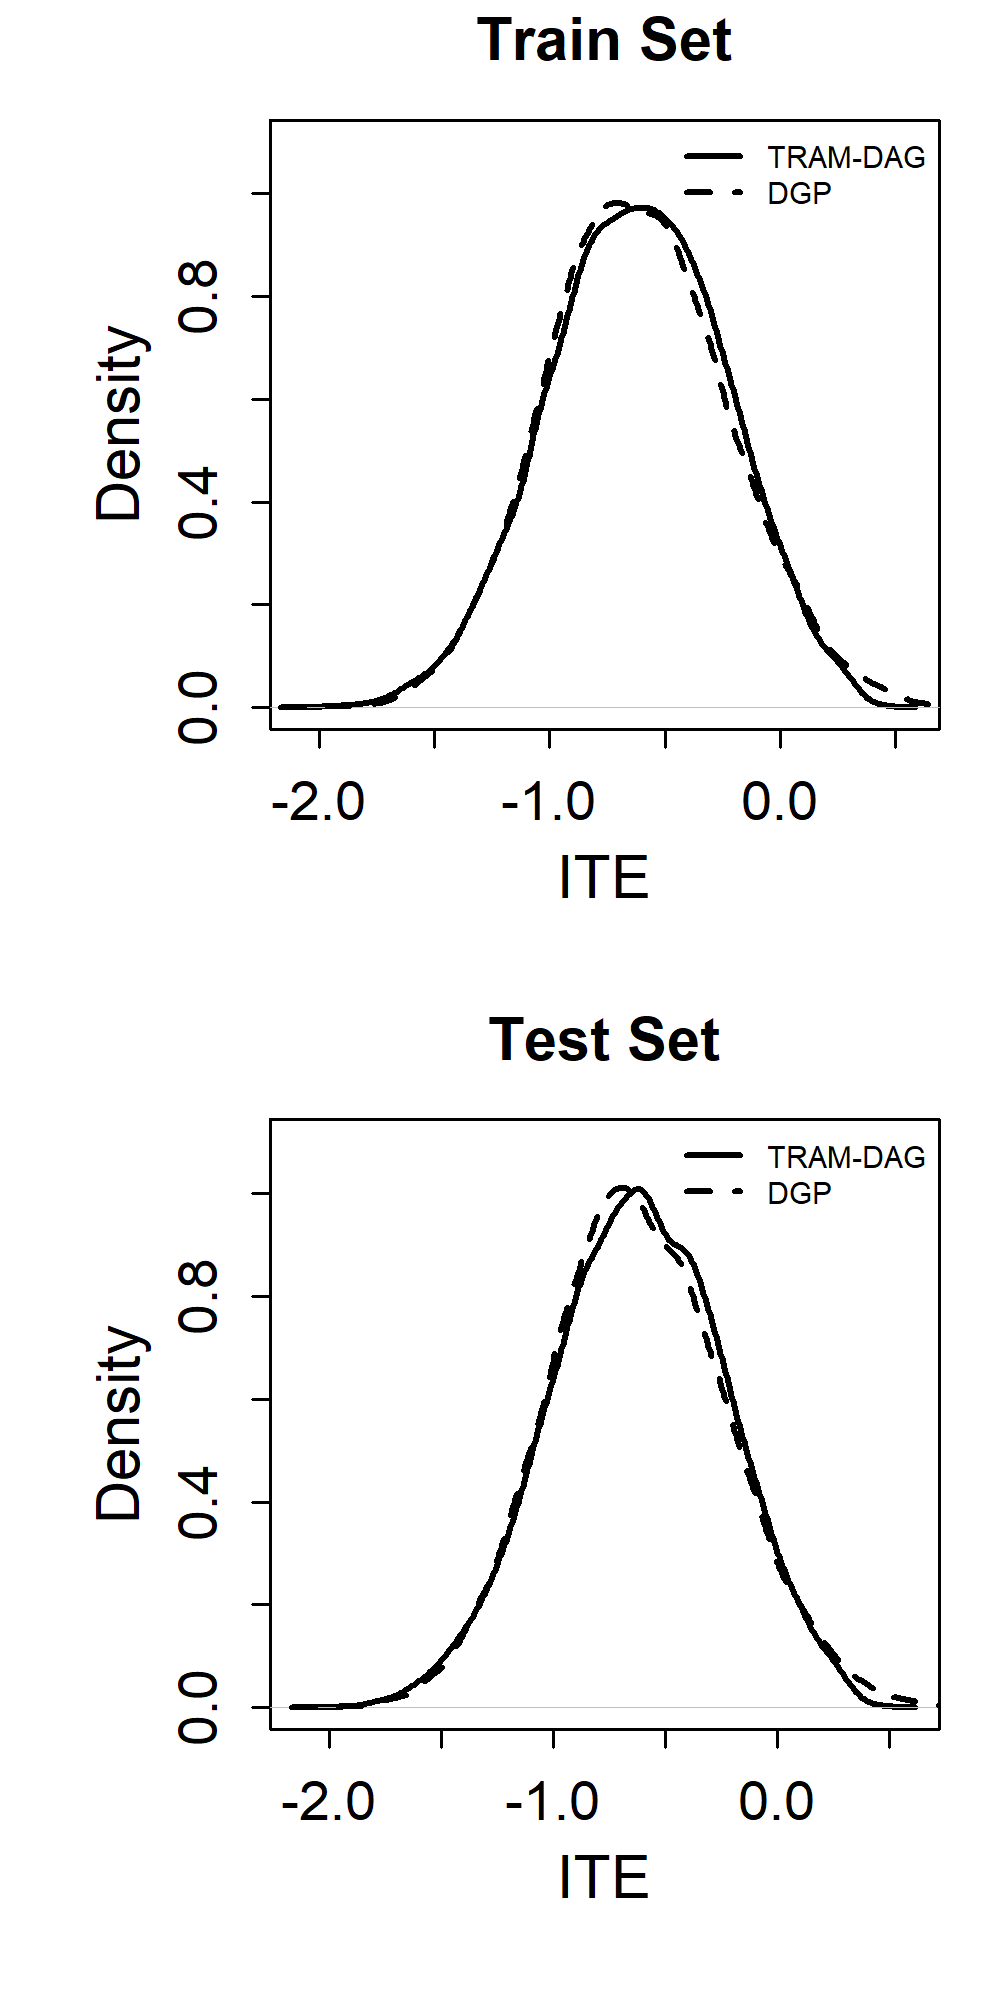
\includegraphics[width=0.33\textwidth]{img/results/rct_scenario1_ITE_densities_train_test.png}
\vspace{-17pt}
\caption{Densities of the estimated ITEs compared to the true ITEs in the training and test datasets for Scenario (1), which includes direct and interaction effects. Left: Observational; Right: RCT setting.}
\label{fig:scenario1_ite_densities_train_test}
\end{figure}






\begin{figure}[htbp]
\centering
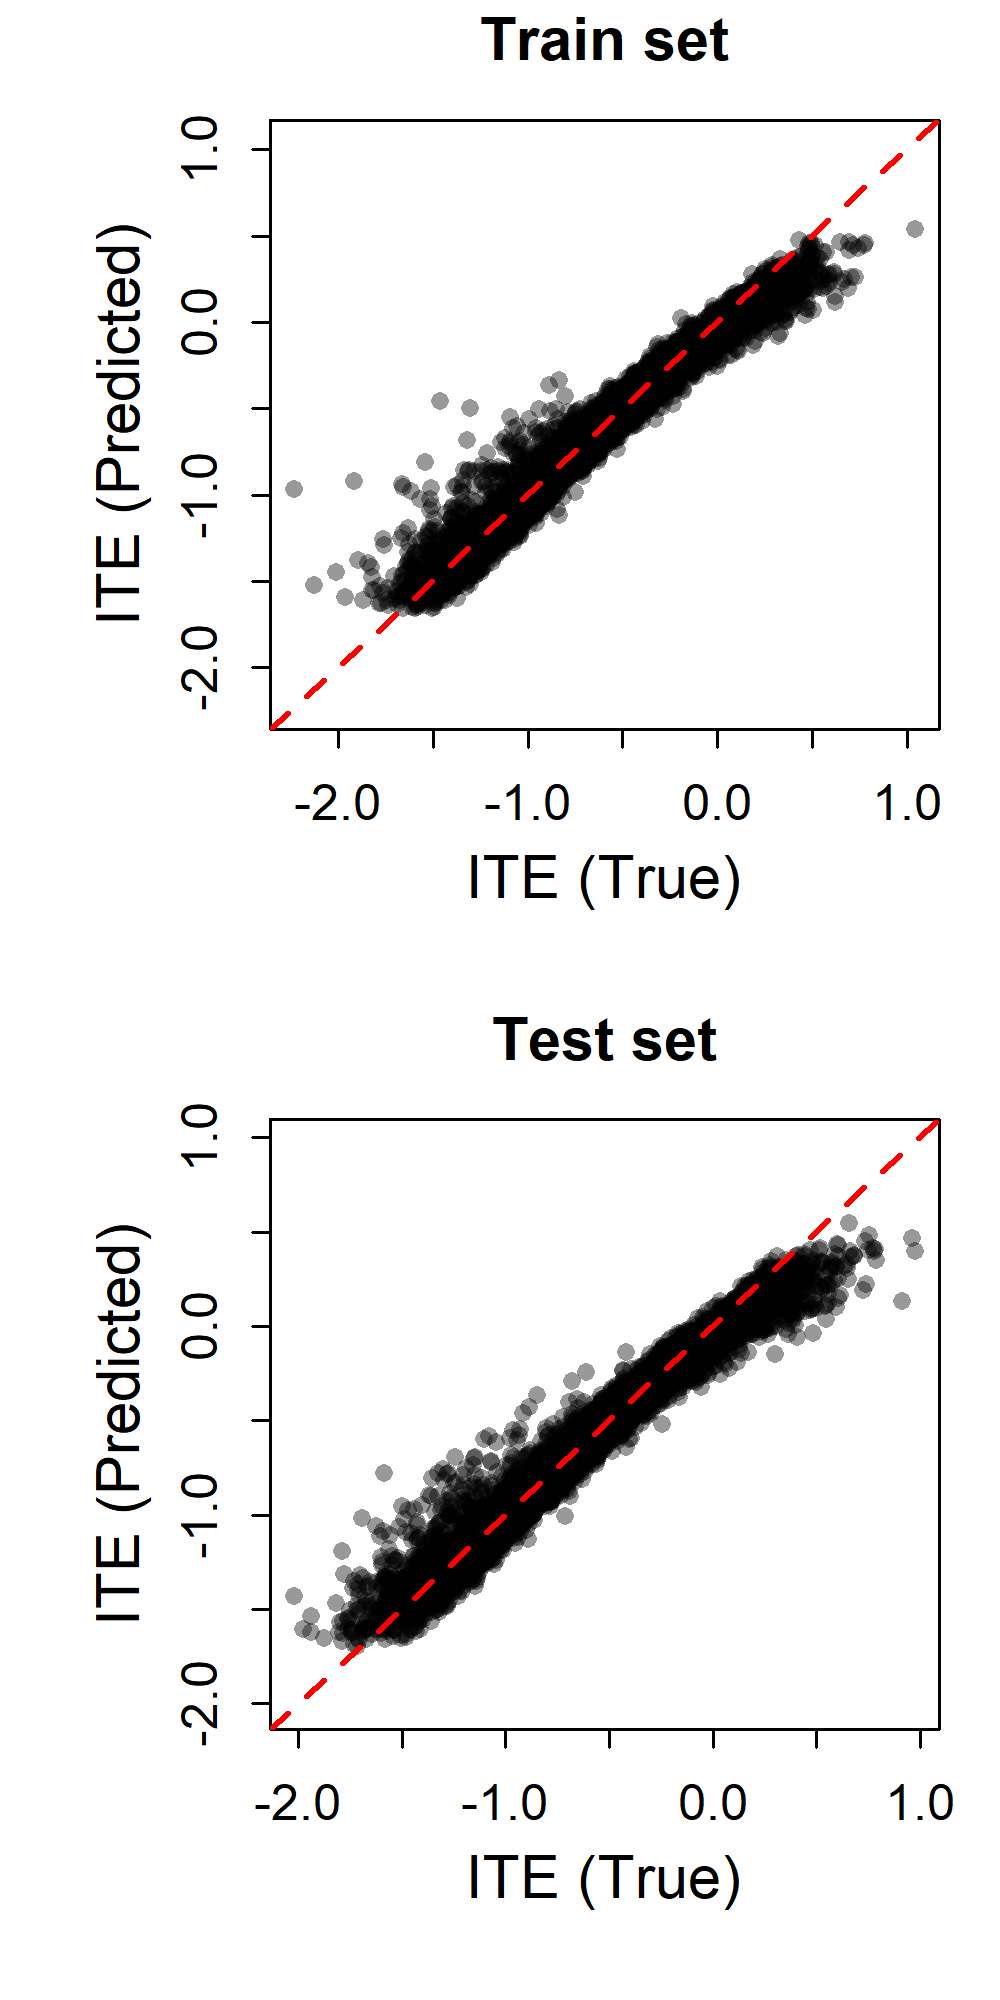
\includegraphics[width=0.33\textwidth]{img/results/observ_scenario1_ITE_scatter_train_test.png} 
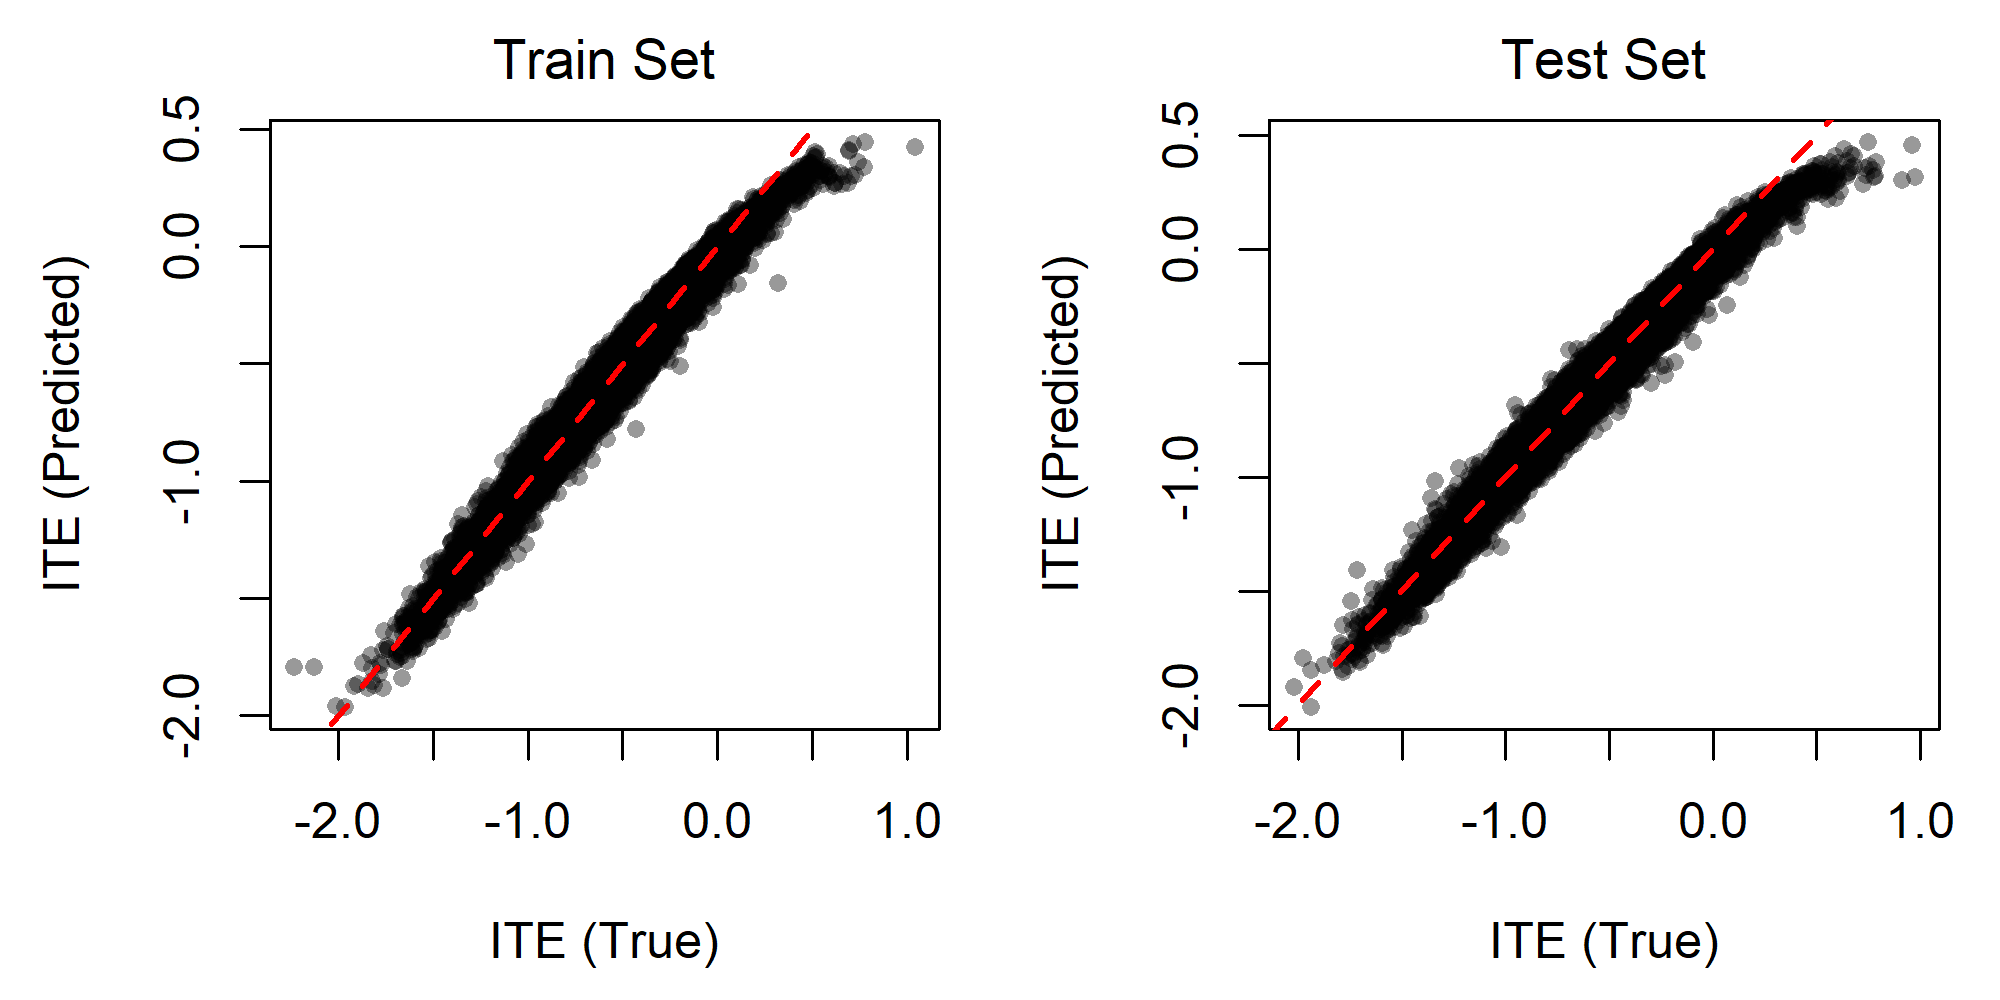
\includegraphics[width=0.33\textwidth]{img/results/rct_scenario1_ITE_scatter_train_test.png}
\vspace{-17pt}
\caption{Scatterplots of estimated ITEs vs. true ITEs in the training and test datasets for Scenario (1), which includes direct and interaction effects. Left: Observational; Right: RCT setting.}
\label{fig:scenario1_ite_scatter_train_test}
\end{figure}



% 
% \begin{figure}[htbp]
% \centering
% 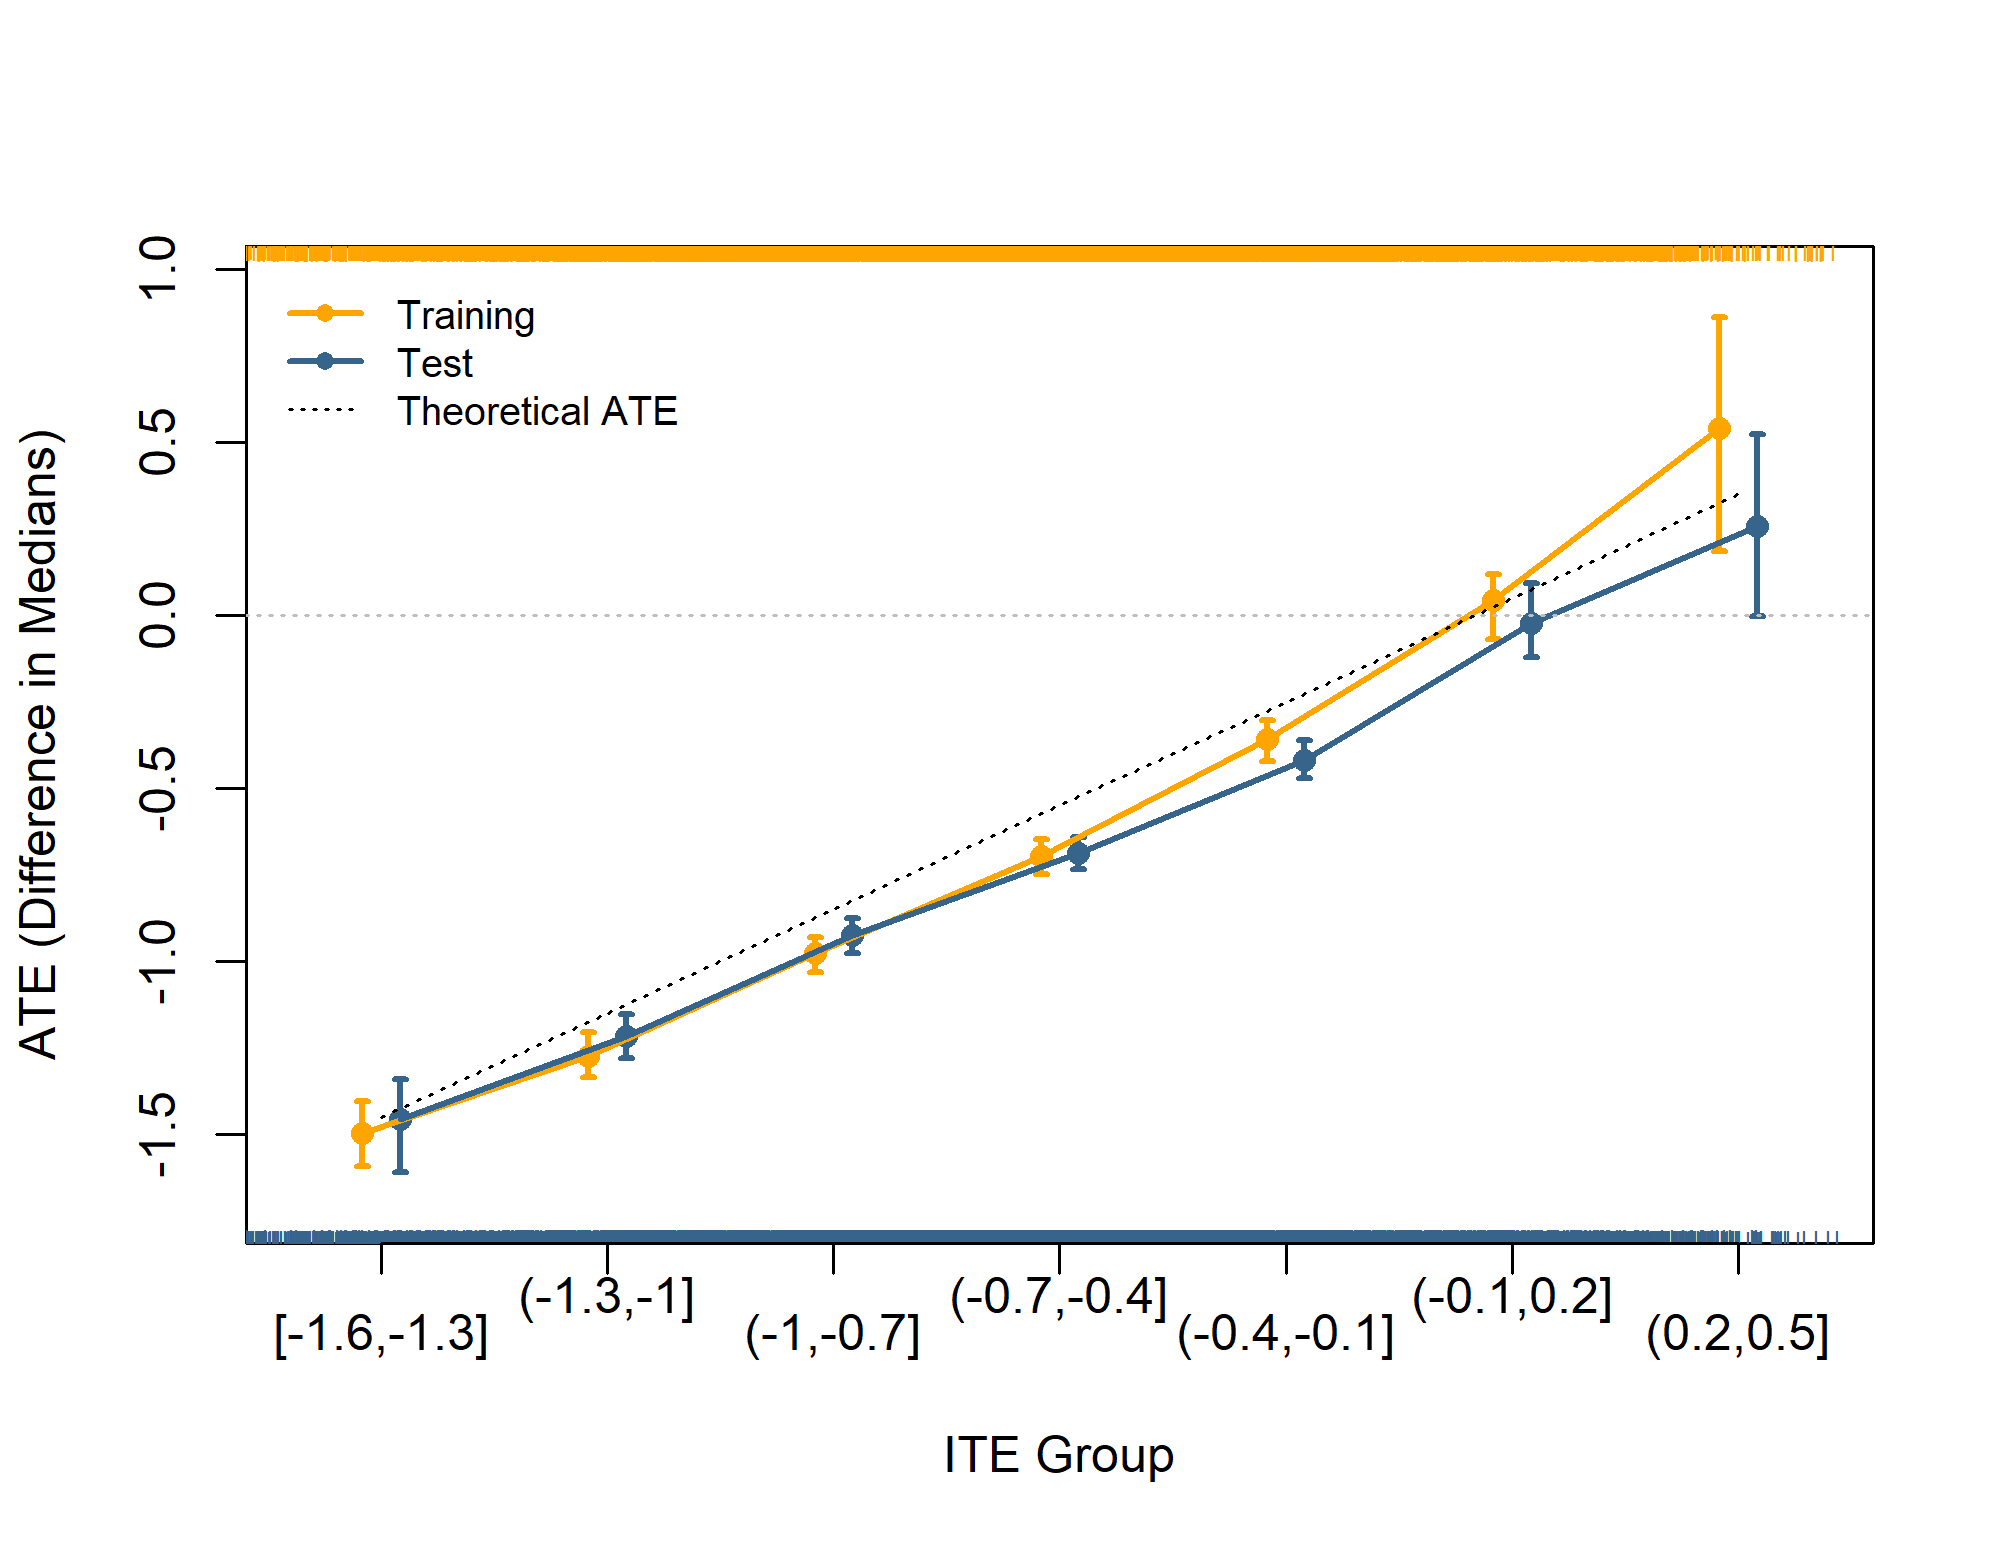
\includegraphics[width=0.45\textwidth]{img/results/observ_scenario1_ITE_ATE.png}
% 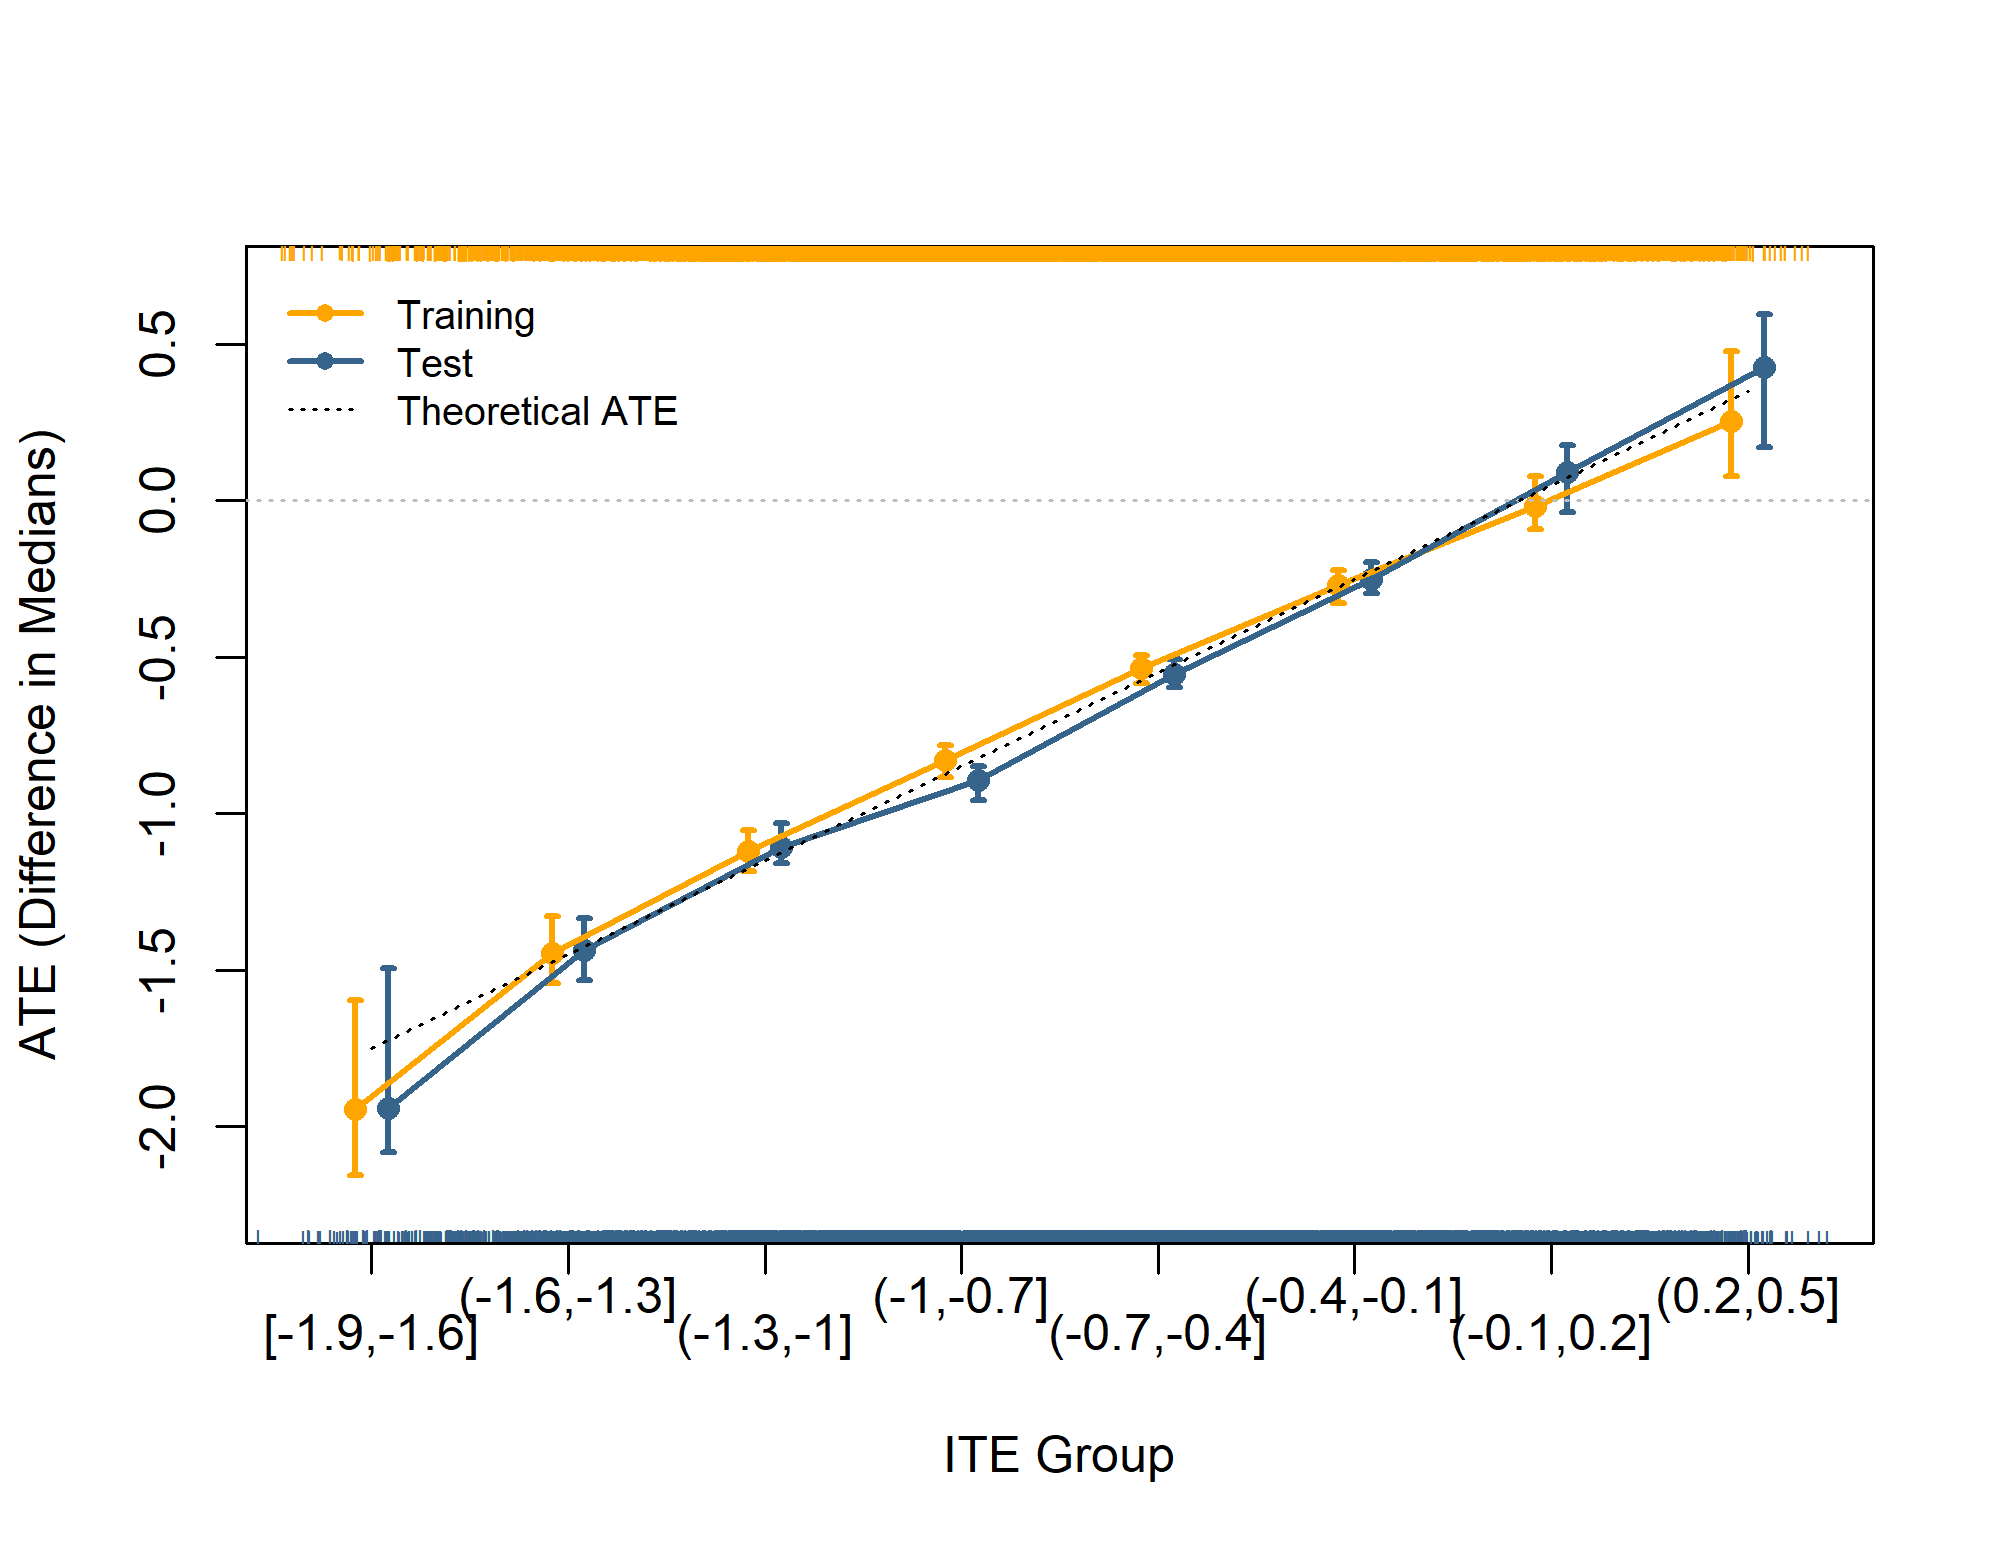
\includegraphics[width=0.45\textwidth]{img/results/rct_scenario1_ITE_ATE.png}
% \caption{ITE-ATE plots for Scenario (1), which includes direct and interaction effects. Individuals are grouped into bins based on their estimated ITEs, and within each bin, the ATE is calculated as the difference in medians of the observed outcomes under the two treatments. 95\% bootstrap confidence intervals indicate the uncertainty. Left: Observational; Right: RCT setting.}
% \label{fig:scenario1_ite_cATE}
% \end{figure}


\begin{figure}[htbp]
\centering
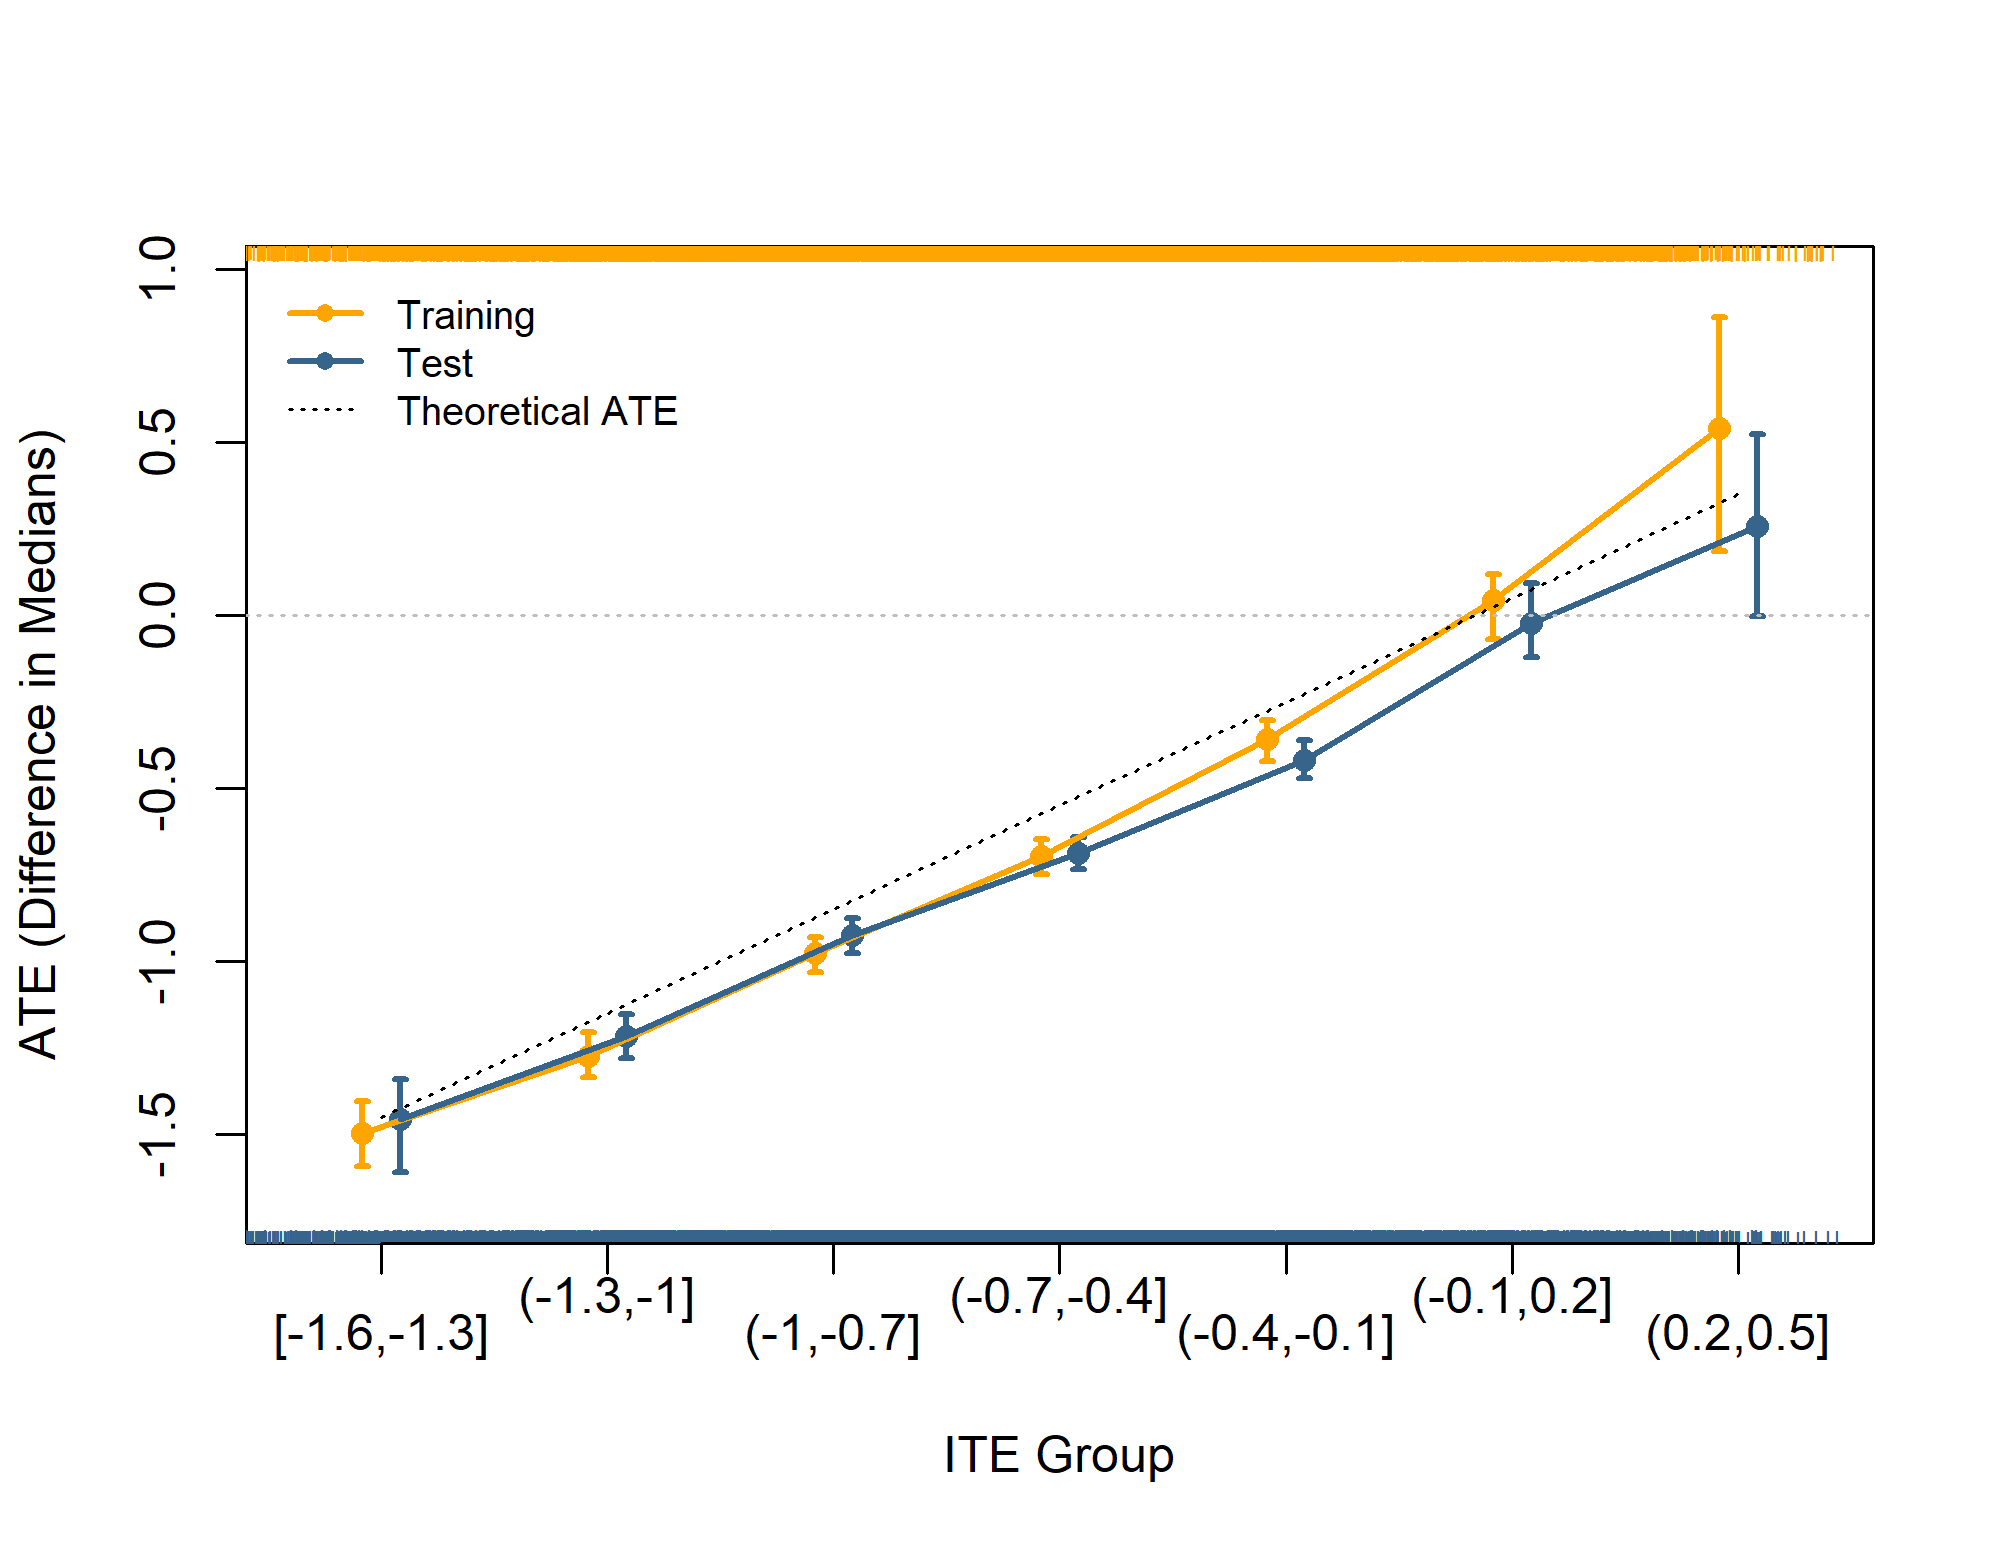
\includegraphics[width=0.8\textwidth]{img/results/observ_scenario1_ITE_ATE.png}
\vspace{-15pt}
\caption{ITE-ATE plot for Scenario (1) in the observatinal setting, which includes direct and interaction effects. Individuals are grouped into bins based on their estimated ITEs, and within each bin, the ATE is calculated as the difference in medians of the observed outcomes under the two treatments. 95\% bootstrap confidence intervals indicate the uncertainty.}
\label{fig:observ_scenario1_ite_ATE}
\end{figure}


\begin{figure}[htbp]
\centering
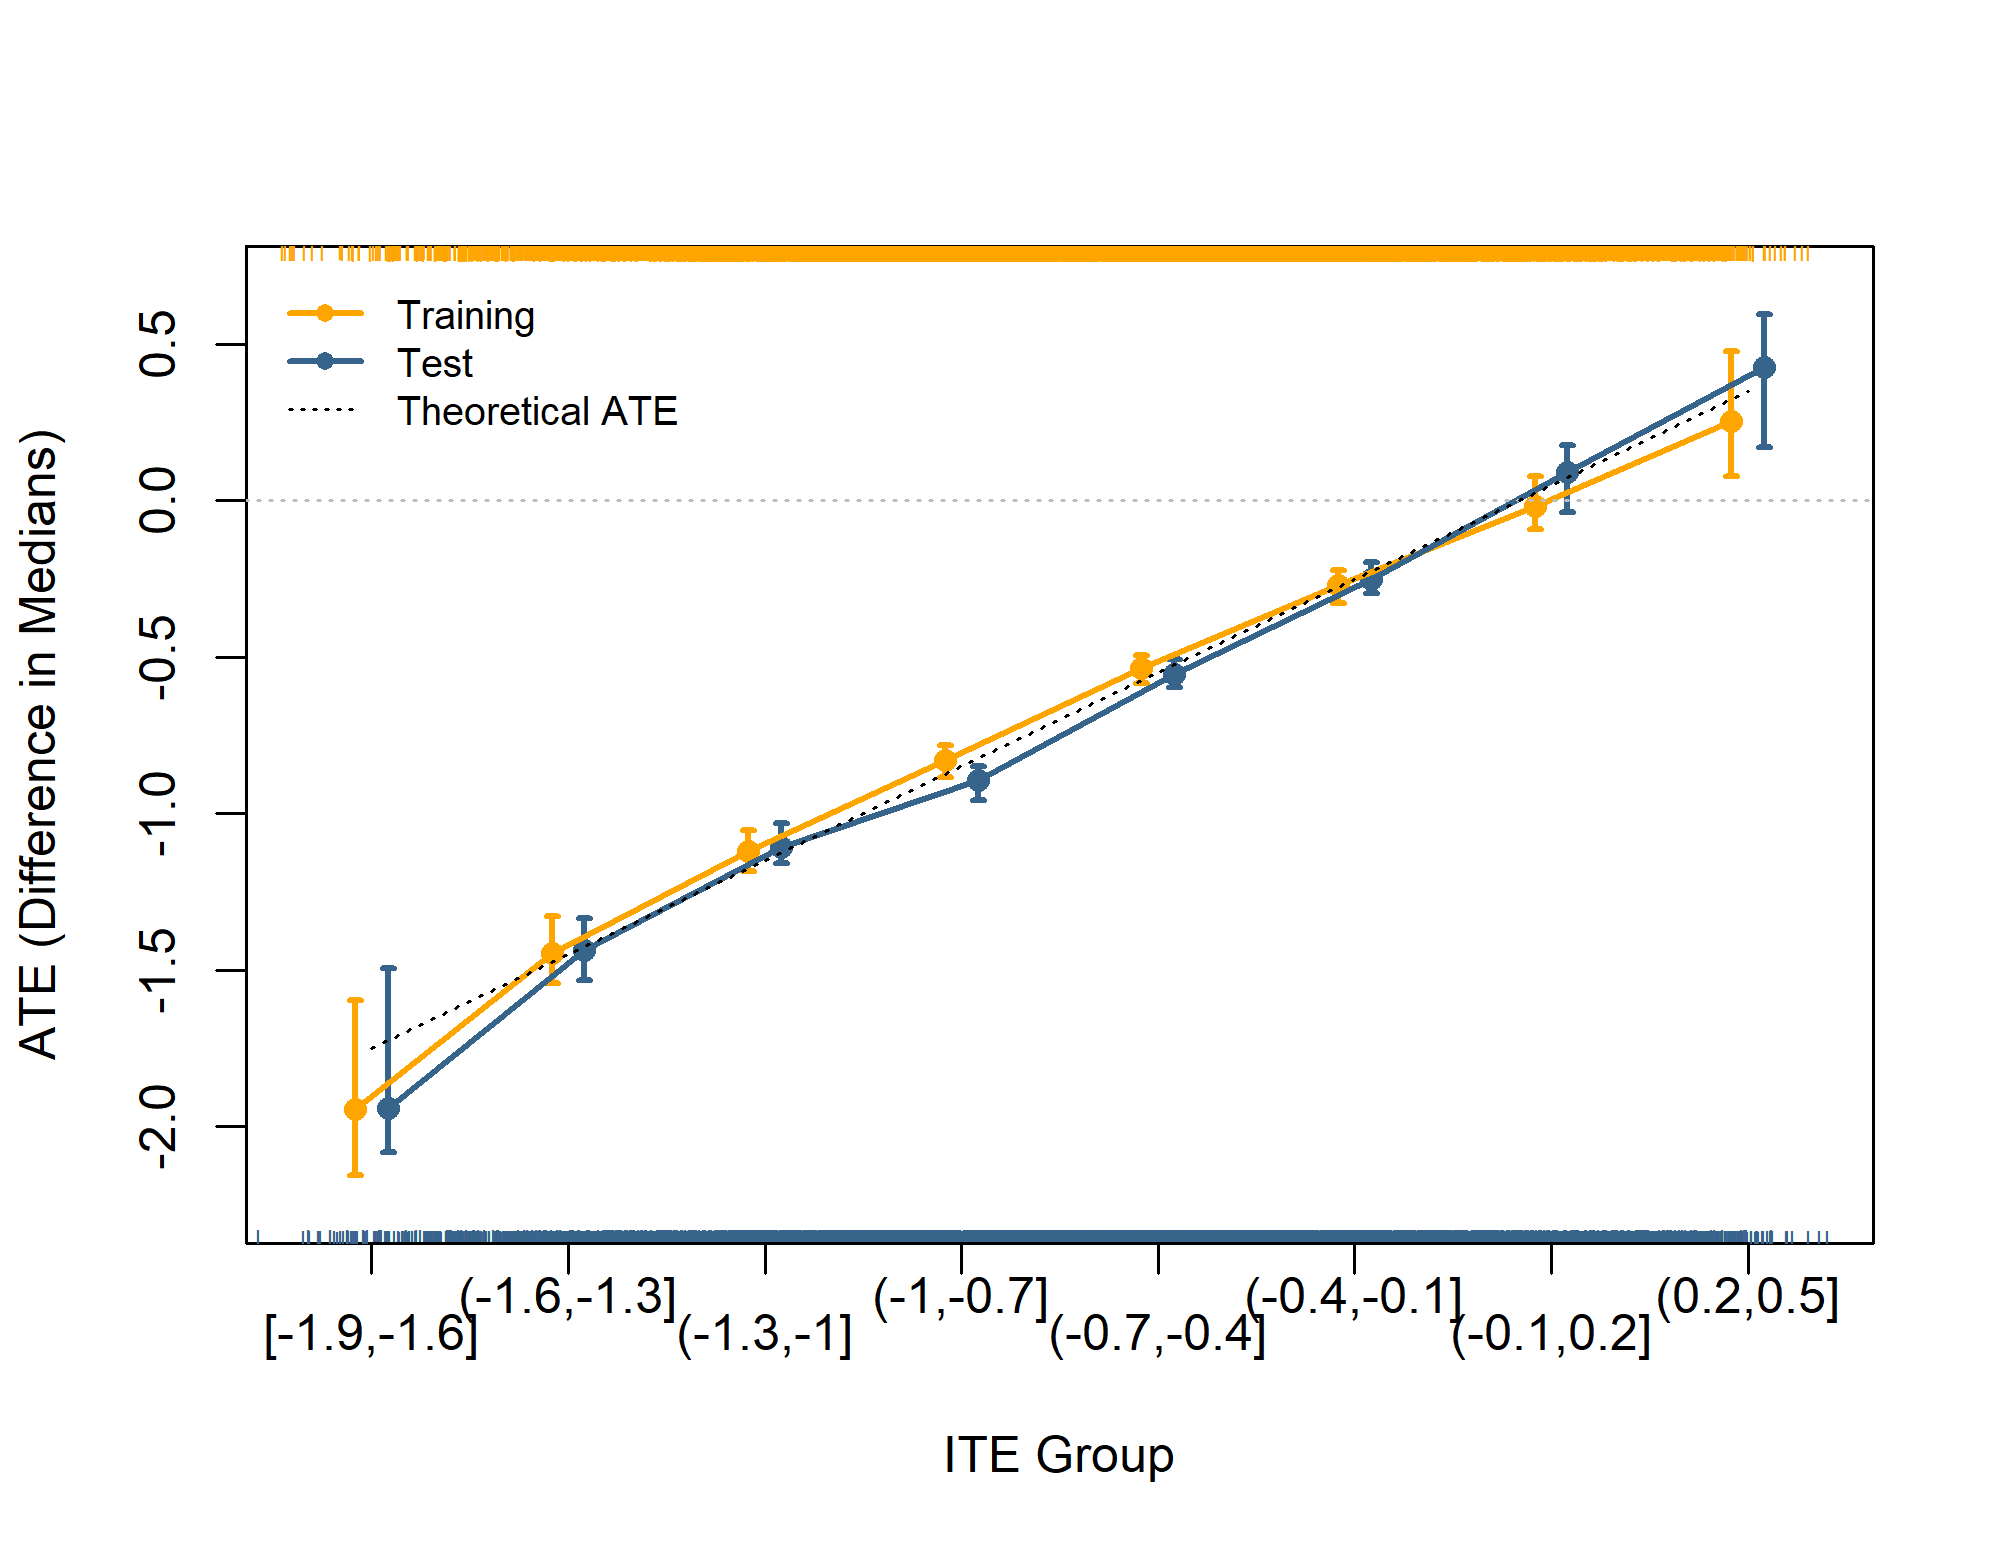
\includegraphics[width=0.8\textwidth]{img/results/rct_scenario1_ITE_ATE.png}
\vspace{-15pt}
\caption{ITE-ATE plot for Scenario (1) in the RCT setting, which includes direct and interaction effects. Individuals are grouped into bins based on their estimated ITEs, and within each bin, the ATE is calculated as the difference in medians of the observed outcomes under the two treatments. 95\% bootstrap confidence intervals indicate the uncertainty.}
\label{fig:rct_scenario1_ite_ATE}
\end{figure}


% start a new page
\clearpage


\subsection{Scenario (2): With direct effect, but no interaction effects}

\begin{figure}[H]
\centering
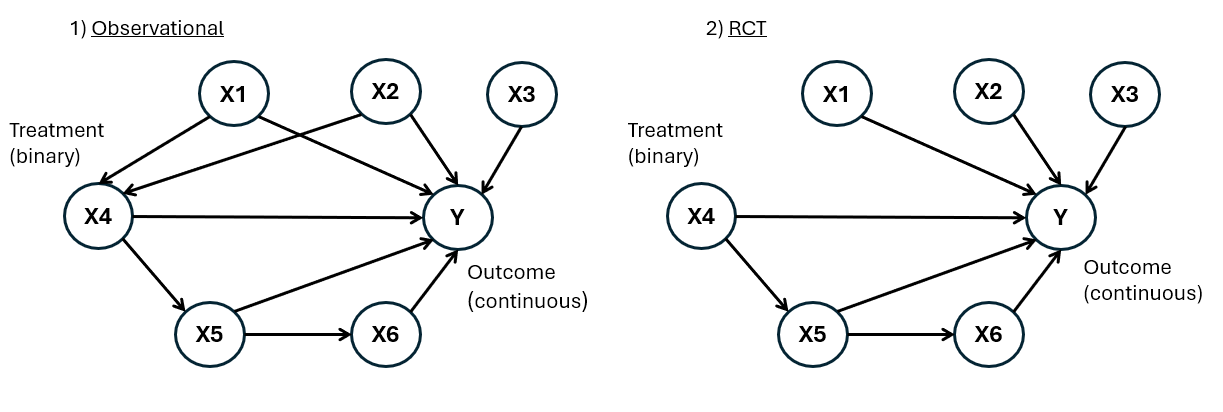
\includegraphics[width=0.85\textwidth]{img/exp4_dag_2.png}
\caption{DAGs for Scenario~(2), which includes a direct effect of the treatment on the outcome, but no interaction effects that would induce treatment effect heterogeneity. Left: Observational setting; Right: RCT setting.}
\label{fig:ite_dag_observational_2}
\end{figure}

Scenario (2) includes a direct effect of the treatment on the outcome, while the coefficients for the interaction terms are set to zero. This results in less heterogeneity in the ITE distribution compared to Scenario (1), as shown in Figure~\ref{fig:scenario2_ite_distribution_dgp}. Why there is still some heterogeneity despite the absence of interactions is discussed in Section~\ref{sec:disc_experiment4}. The observational and interventional densities generated by the fitted TRAM-DAG closely match the true densities defined by the DGP, as illustrated in Figures~\ref{fig:scenario2_sampling_distributions_vertical} and~\ref{fig:scenario2_outcome_distributions}. However, there is a notable difference in variance between the estimated and true ITE distributions, visible in Figures~\ref{fig:scenario2_ite_densities_train_test} and~\ref{fig:scenario2_ite_scatter_train_test}. The ITE-ATE plots in Figures~\ref{fig:observ_scenario2_ite_ATE} and \ref{fig:rct_scenario2_ite_ATE} are less informative than in Scenario (1), as expected given the reduced heterogeneity. Table~\ref{tab:scenario2_ate_comparison} presents the ATE measures for Scenario (2). In the test set of the RCT setting, the ATE based on the true ITEs was -0.633, while the ATE based on the estimated ITEs was -0.586.


\begin{table}[htbp]
\centering
\small
\caption{Scenario (2), including a direct treatment effect but no interaction effects: Comparison of ATE measures across train and test sets for the observational and RCT setting. $\text{Y}_\text{observed}^{(\text{Tr})}$ denotes the observed outcome under the treatment ($\text{Tr}$) actually received. The estimated ATE from $\text{mean}(\text{ITE}_\text{estimated})$ can be directly compared to the true $\text{mean}(\text{ITE}_\text{true})$, whereas comparisons to the empirical ATEs based on outcome differences should be interpreted with caution.}
\label{tab:scenario2_ate_comparison}
\begin{tabular}{l c c c c}
\toprule
\textbf{Measure} & \multicolumn{2}{c}{\textbf{Observational}} & \multicolumn{2}{c}{\textbf{RCT}} \\
\cmidrule(lr){2-3} \cmidrule(lr){4-5}
 & \textbf{Train} & \textbf{Test} & \textbf{Train} & \textbf{Test} \\
\midrule
ATE as $\text{mean}(\text{Y}_\text{observed}^{(1)}) - \text{mean}(\text{Y}_\text{observed}^{(0)})$ 
& NA & NA 
& -0.569 
& -0.572 \\

ATE as $\text{median}(\text{Y}_\text{observed}^{(1)}) - \text{median}(\text{Y}_\text{observed}^{(0)})$  
& NA & NA 
& -0.629 
& -0.639 \\

ATE as mean(ITE$_\text{true}$)  
& -0.633 
& -0.633 
& -0.633 
& -0.633 \\

ATE as mean(ITE$_\text{estimated}$) 
& -0.645 
& -0.644 
& -0.587 
& -0.586 \\
\bottomrule
\end{tabular}
\end{table}

% 
% \begin{table}[htbp]
% \centering
% \small
% \caption{Scenario (2), including a direct treatment but no interaction effects: Comparison of ATE measures across train and test sets for the observational and RCT setting.}
% \label{tab:scenario2_ate_comparison_old}
% \begin{tabular}{l c c c c}
% \toprule
% \textbf{Measure} & \multicolumn{2}{c}{\textbf{Observational}} & \multicolumn{2}{c}{\textbf{RCT}} \\
% \cmidrule(lr){2-3} \cmidrule(lr){4-5}
%  & \textbf{Train} & \textbf{Test} & \textbf{Train} & \textbf{Test} \\
% \midrule
% ATE as $\text{mean}(\text{Y}_\text{observed}^{(1)}) - \text{mean}(\text{Y}_\text{observed}^{(0)})$ & NA & NA & round(rct_scenario2$dev_ATE_observed_Y_mean_diff, 3) & round(rct_scenario2$val_ATE_observed_Y_mean_diff, 3) \\
% ATE as $\text{median}(\text{Y}_\text{observed}^{(1)}) - \text{median}(\text{Y}_\text{observed}^{(0)})$  & NA & NA & round(rct_scenario2$dev_ATE_observed_Y_median_diff, 3) & round(rct_scenario2$val_ATE_observed_Y_median_diff, 3) \\
% ATE as mean(ITE$_\text{true}$)  & round(observ_scenario2$dev_ITE_median_average, 3) & round(observ_scenario2$val_ITE_median_average, 3) & round(rct_scenario2$dev_ITE_median_average, 3) & round(rct_scenario2$val_ITE_median_average, 3) \\
% ATE as mean(ITE$_\text{estimated}$) & round(observ_scenario2$dev_ITE_median_pred_average, 3) & round(observ_scenario2$val_ITE_median_pred_average, 3) & round(rct_scenario2$dev_ITE_median_pred_average, 3) & round(rct_scenario2$val_ITE_median_pred_average, 3) \\
% \bottomrule
% \end{tabular}
% \end{table}



\begin{figure}[htbp]
\centering
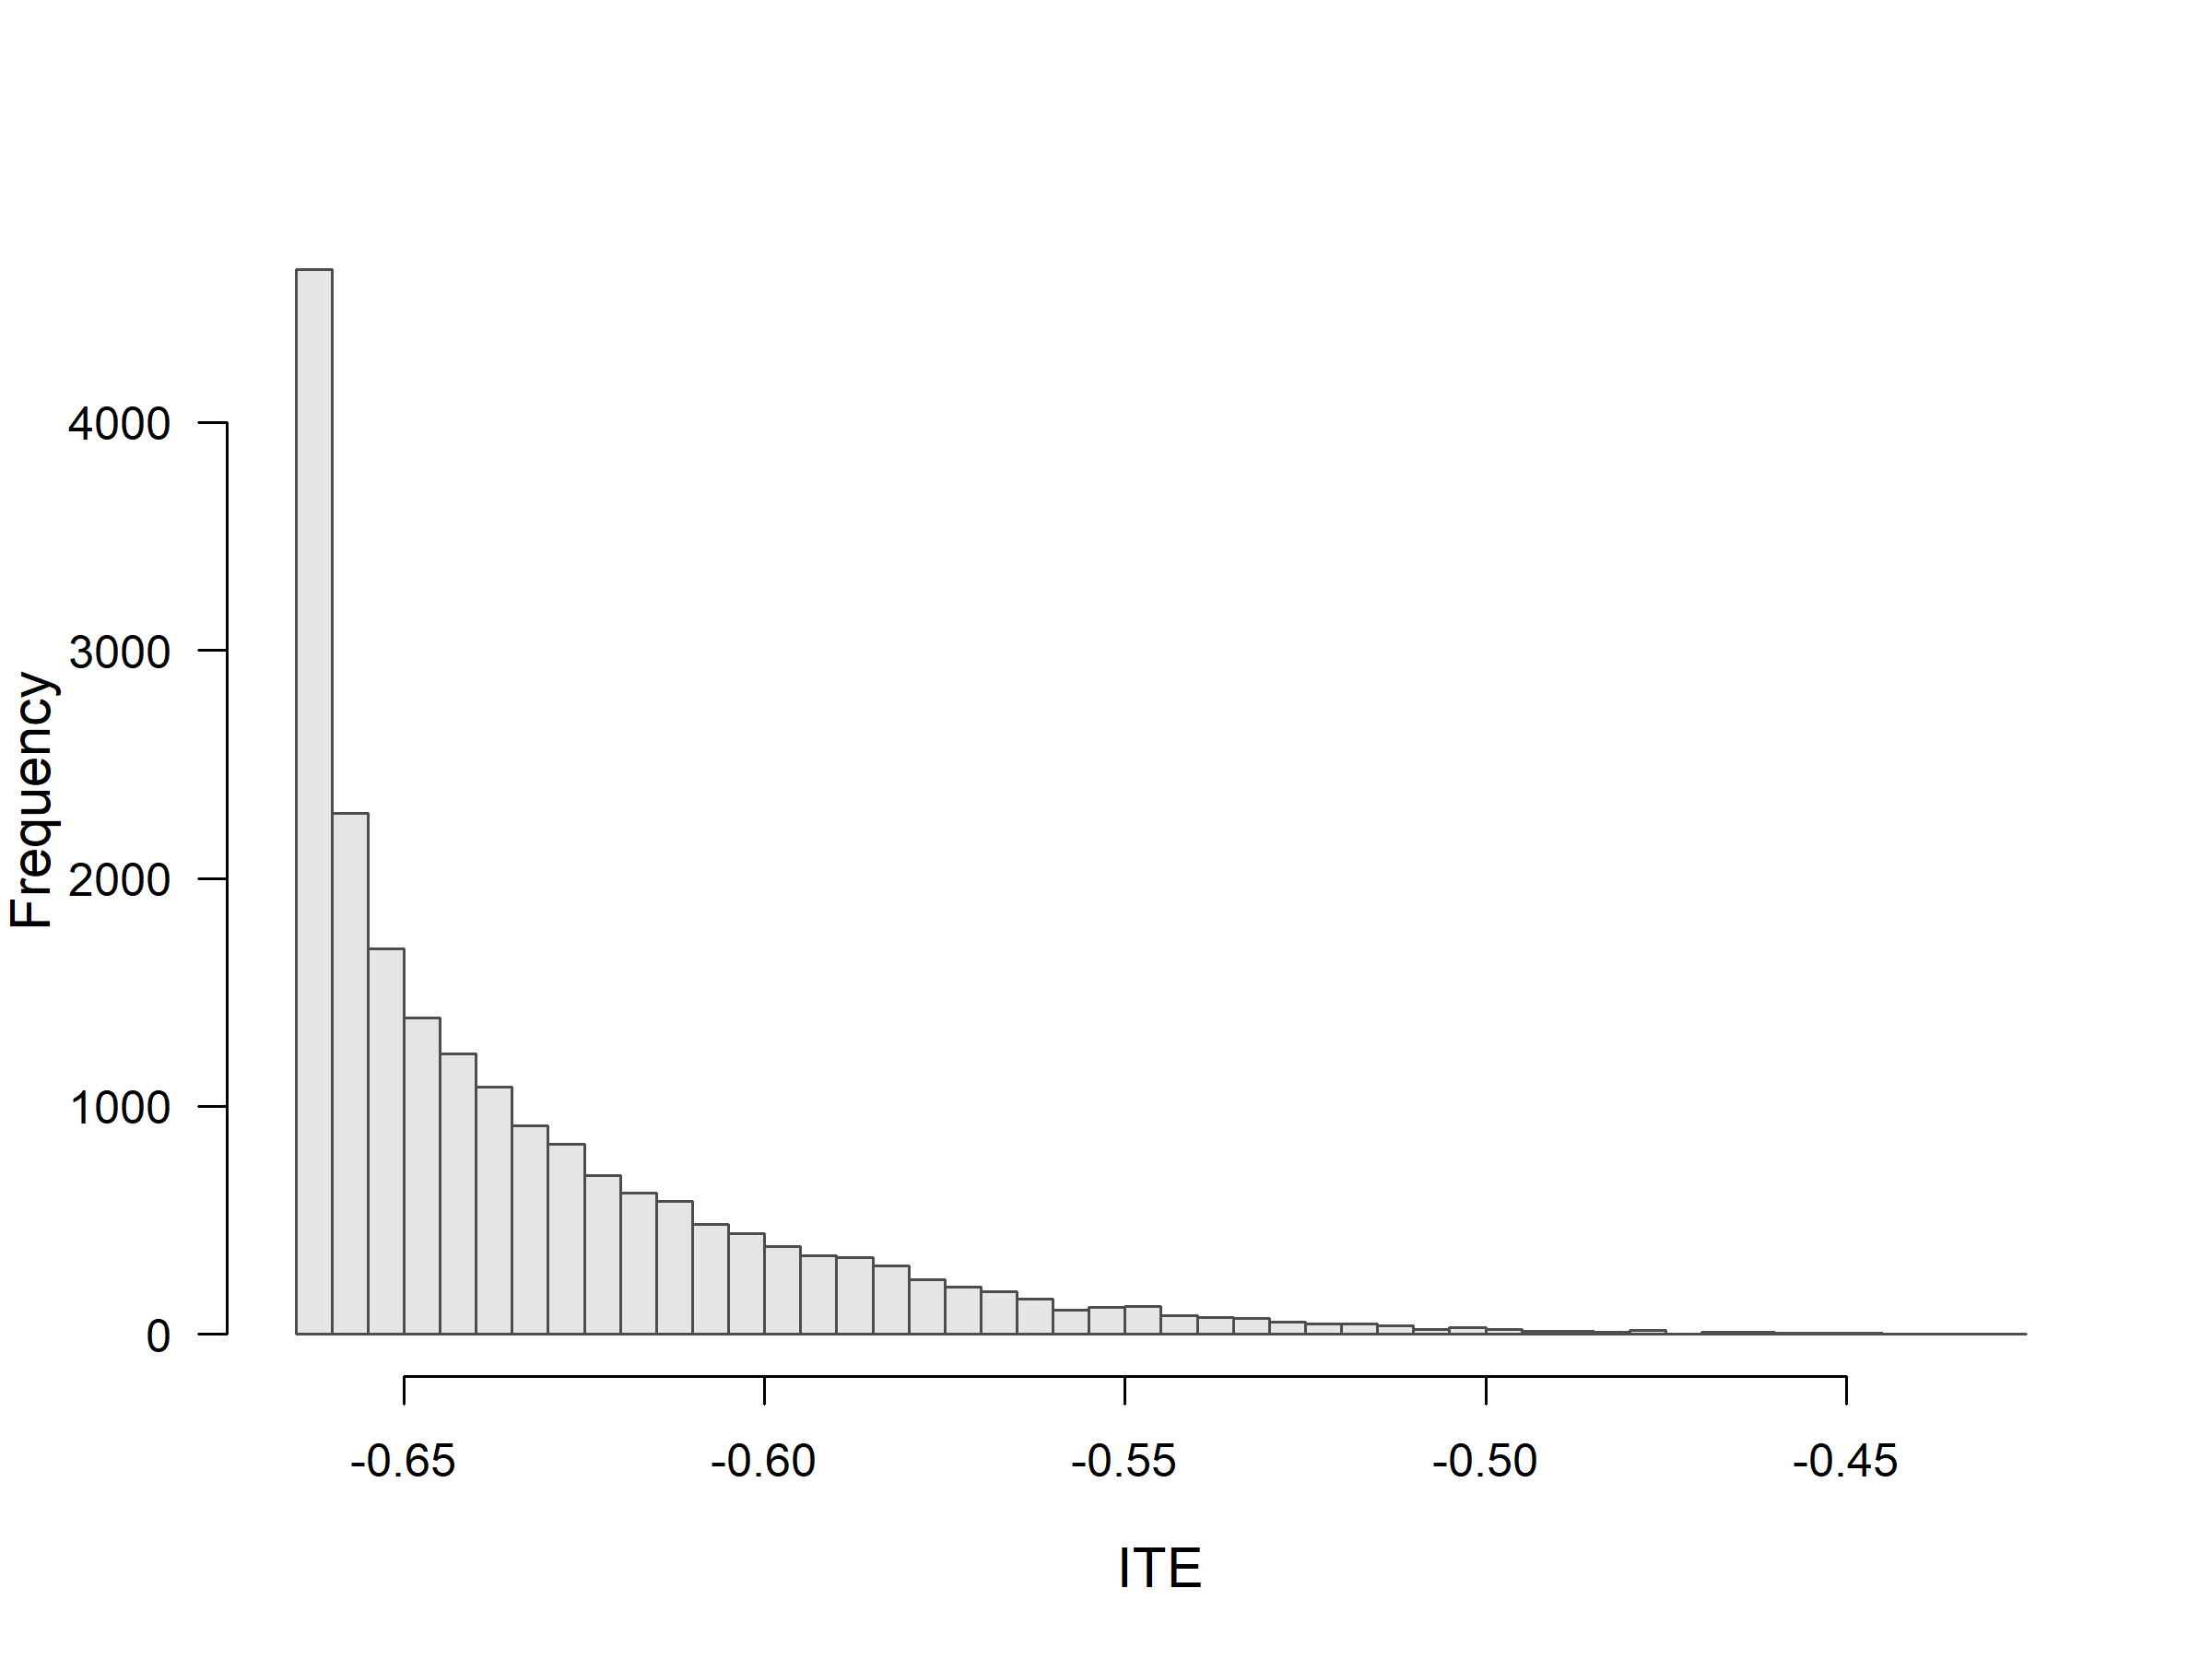
\includegraphics[width=0.7\textwidth]{img/results/observ_scenario2_ite_distribution_dgp.png}
\caption{True ITE distribution resulting from the DGP for Scenario~(2), which includes a direct treatment effect but no interaction effects. The true ITEs are identical in the observational and RCT settings, as they depend only on the potential outcomes under both treatment allocations.}
\label{fig:scenario2_ite_distribution_dgp}
\end{figure}



\begin{figure}[htbp]
\centering
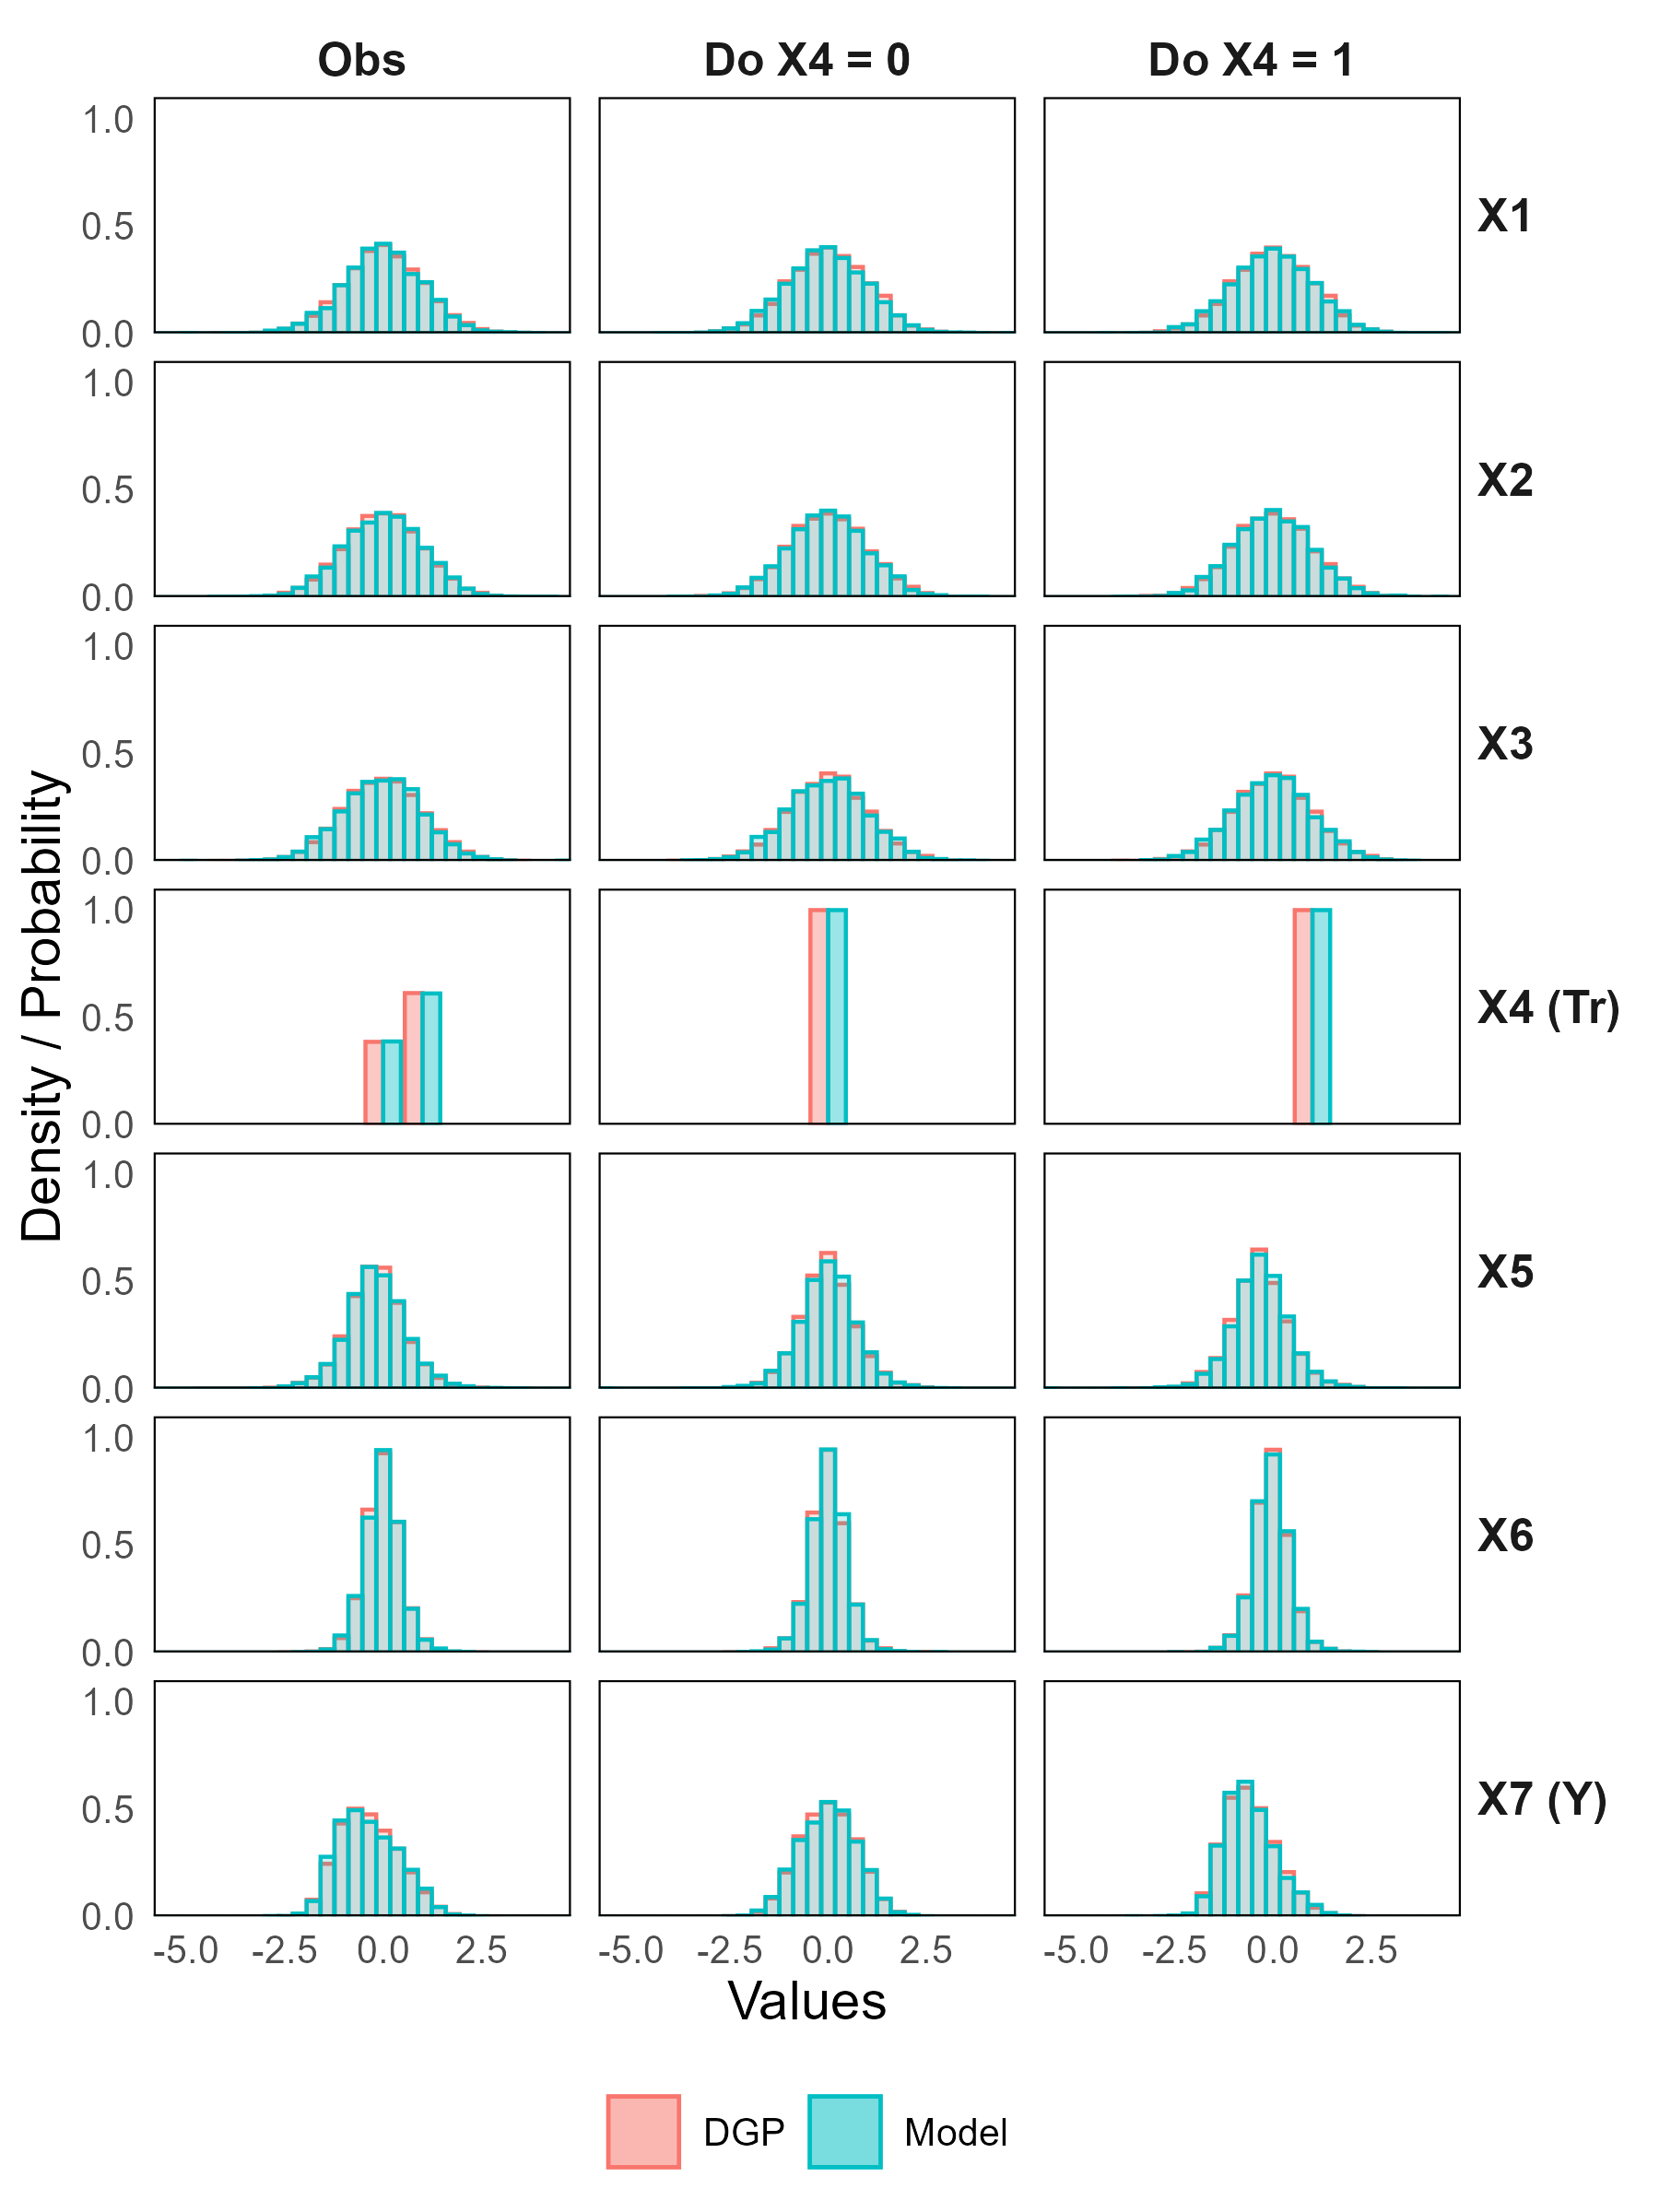
\includegraphics[width=0.45\textwidth]{img/results/observ_scenario2_sampling_distributions_vertical.png}
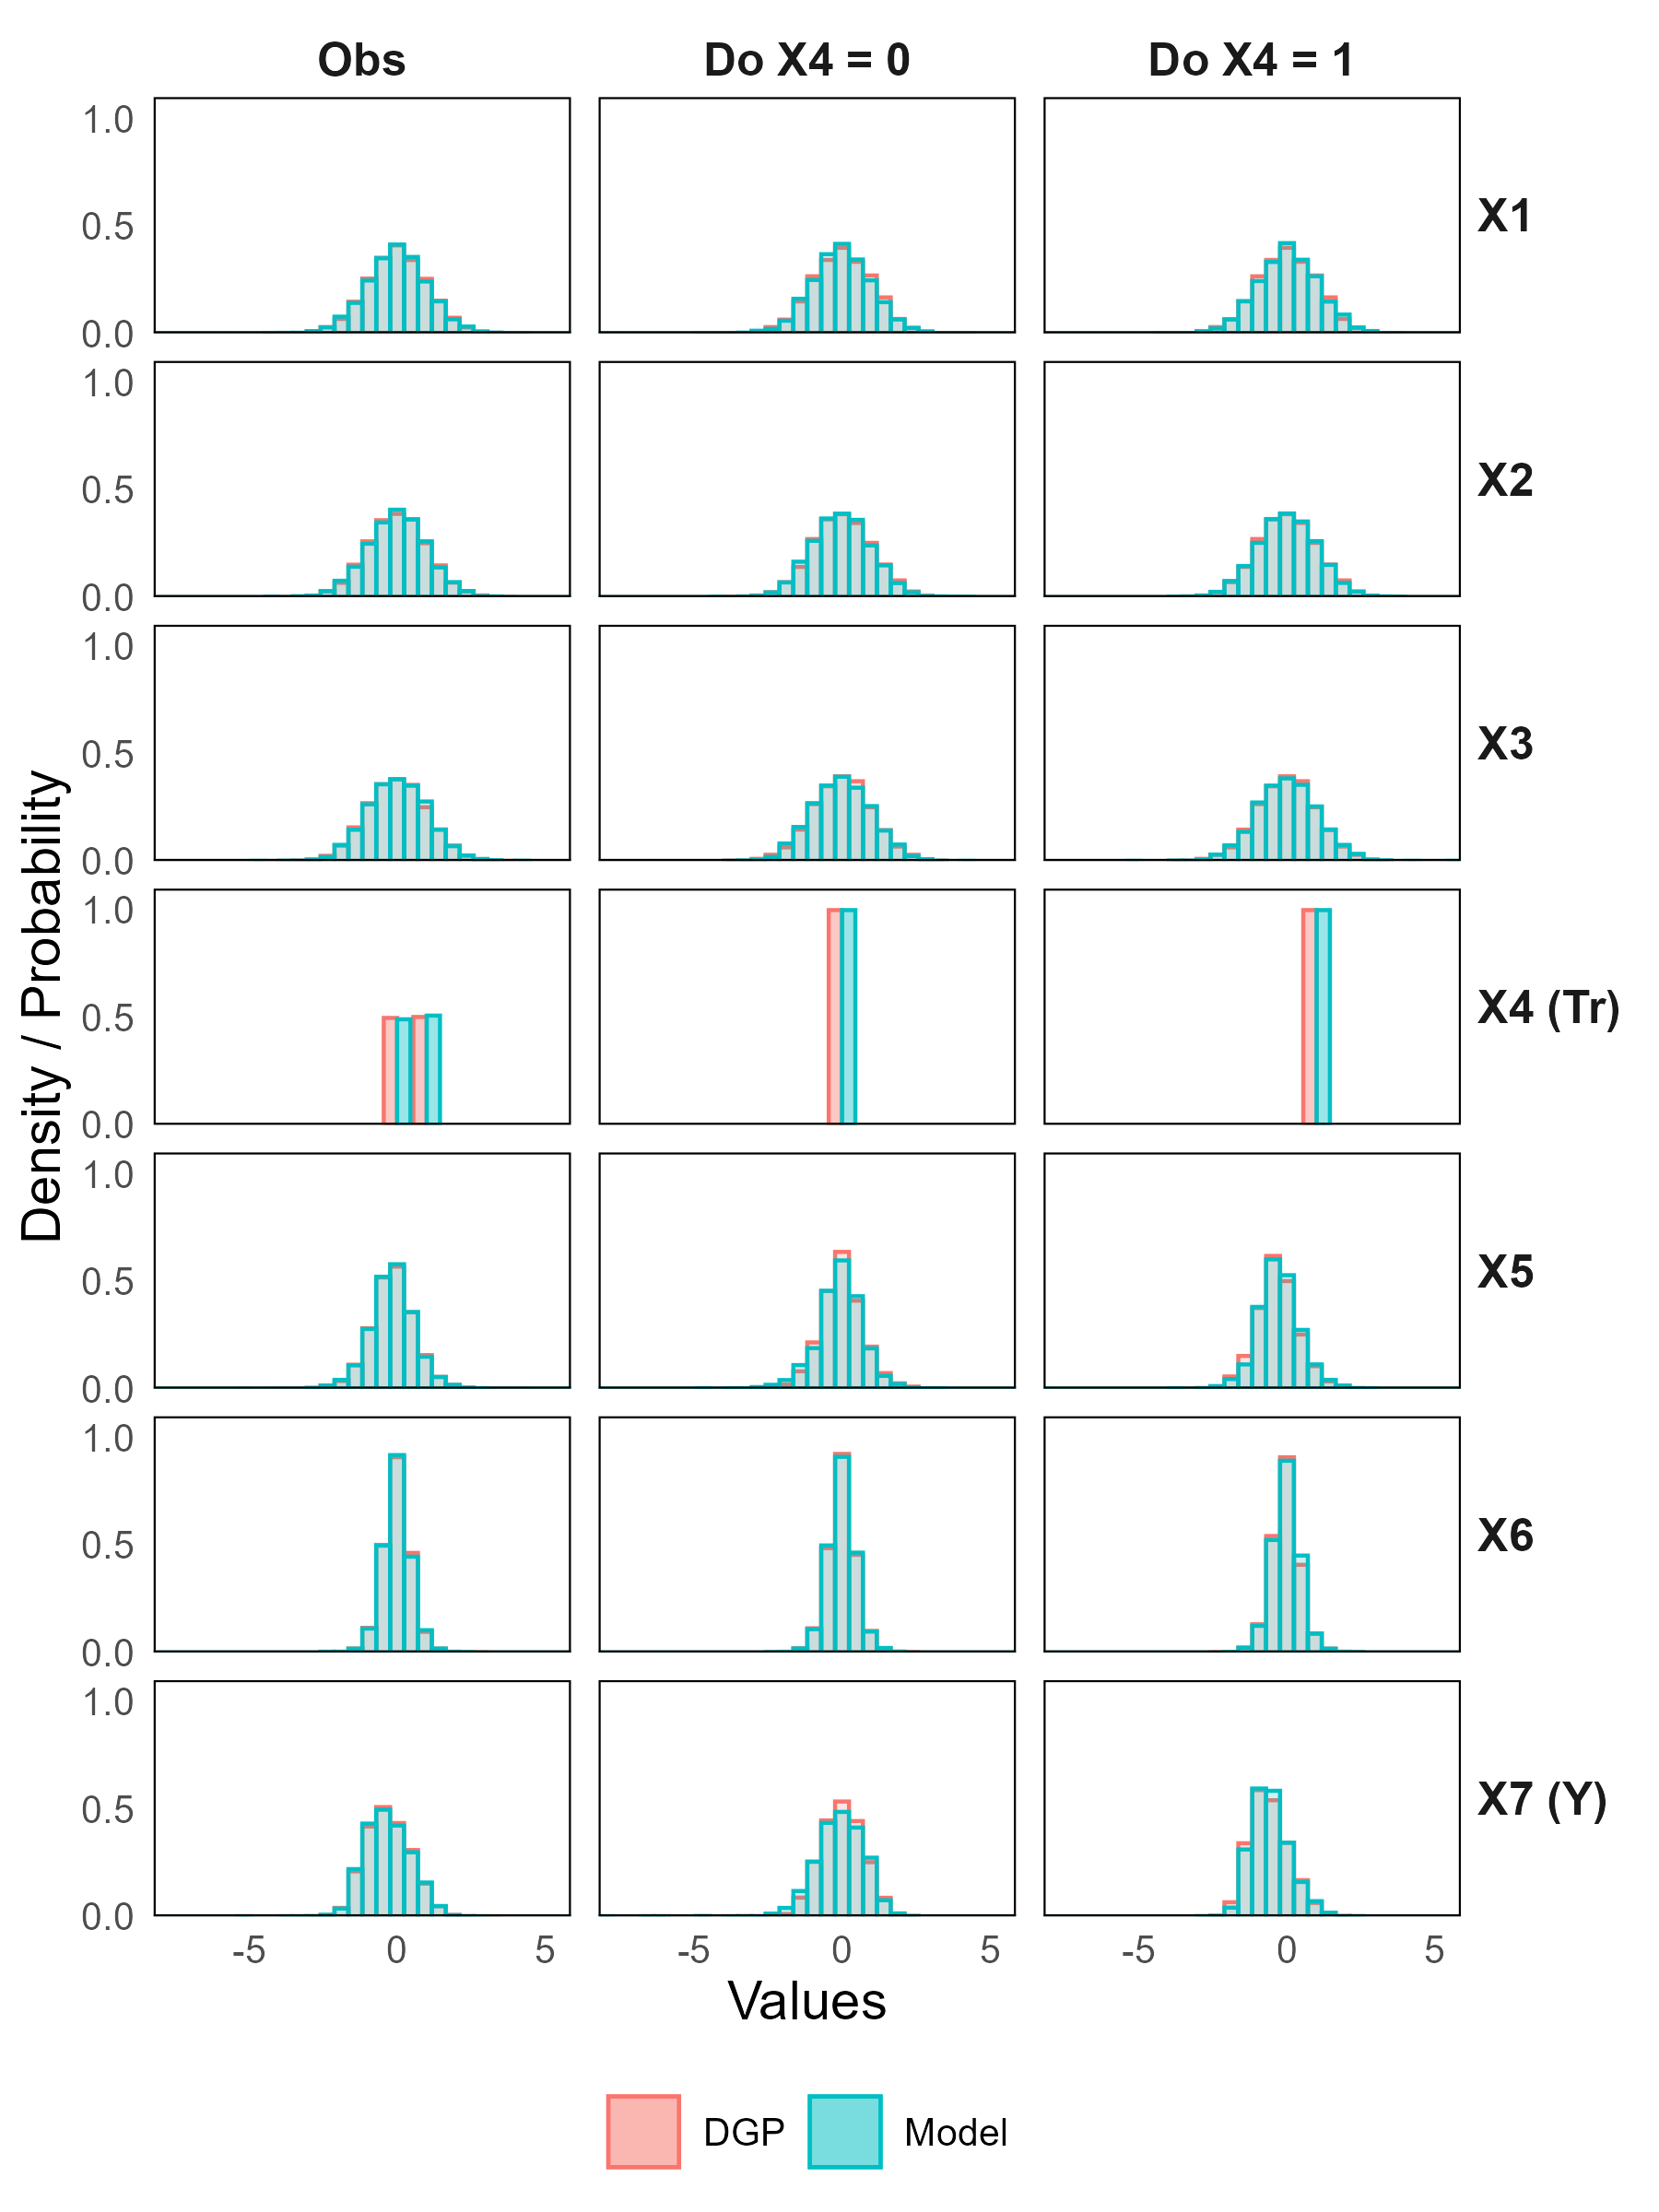
\includegraphics[width=0.45\textwidth]{img/results/rct_scenario2_sampling_distributions_vertical.png}
\caption{Marginal distributions of variables from the DGP and samples generated by the fitted TRAM-DAG for Scenario~(2), which includes a direct treatment effect but no interaction effects. The distributions are shown as observed (Obs), under control intervention (do($X_4 = 0$)), and under treatment intervention (do($X_4 = 1$)). Left: Observational; Right: RCT setting.}
\label{fig:scenario2_sampling_distributions_vertical}
\end{figure}


\begin{figure}[htbp]
\centering
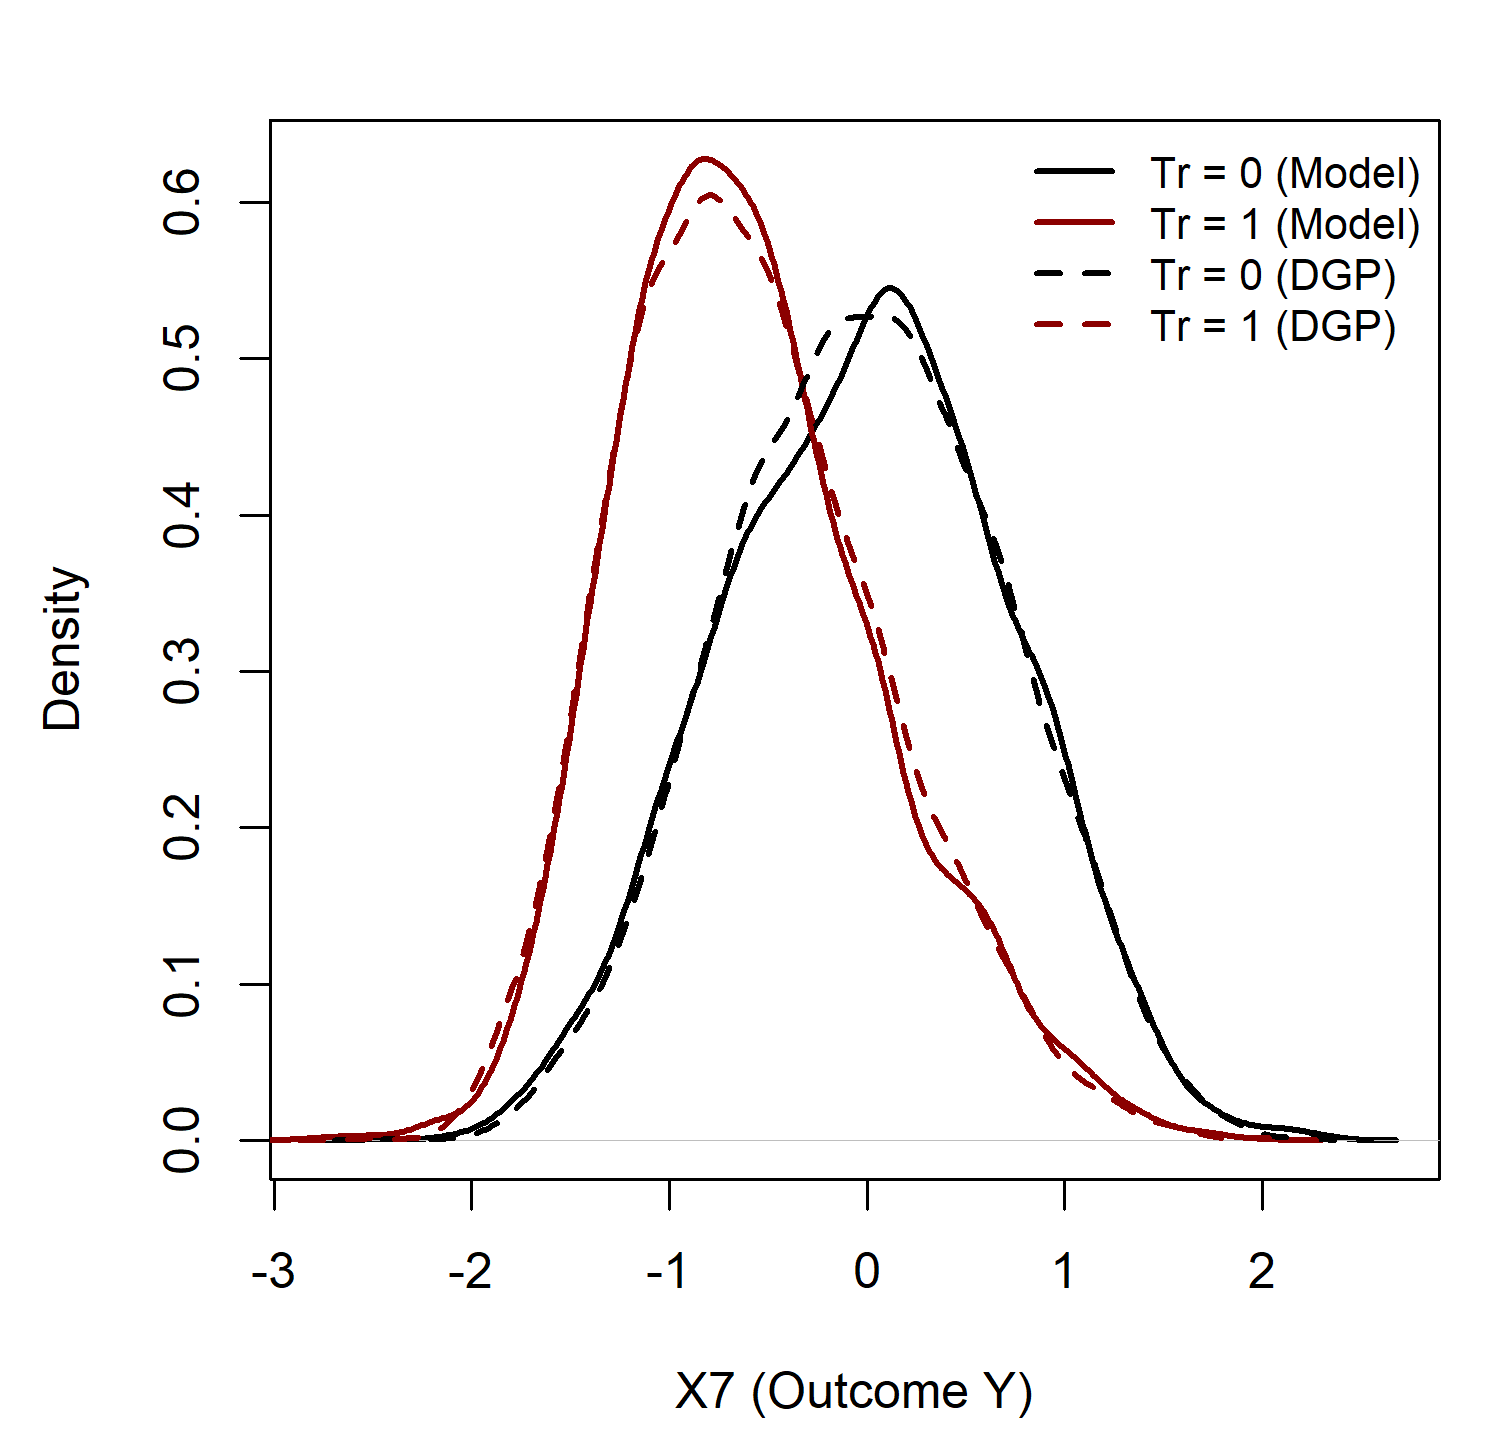
\includegraphics[width=0.45\textwidth]{img/results/observ_scenario2_X7_treatment_densities.png}
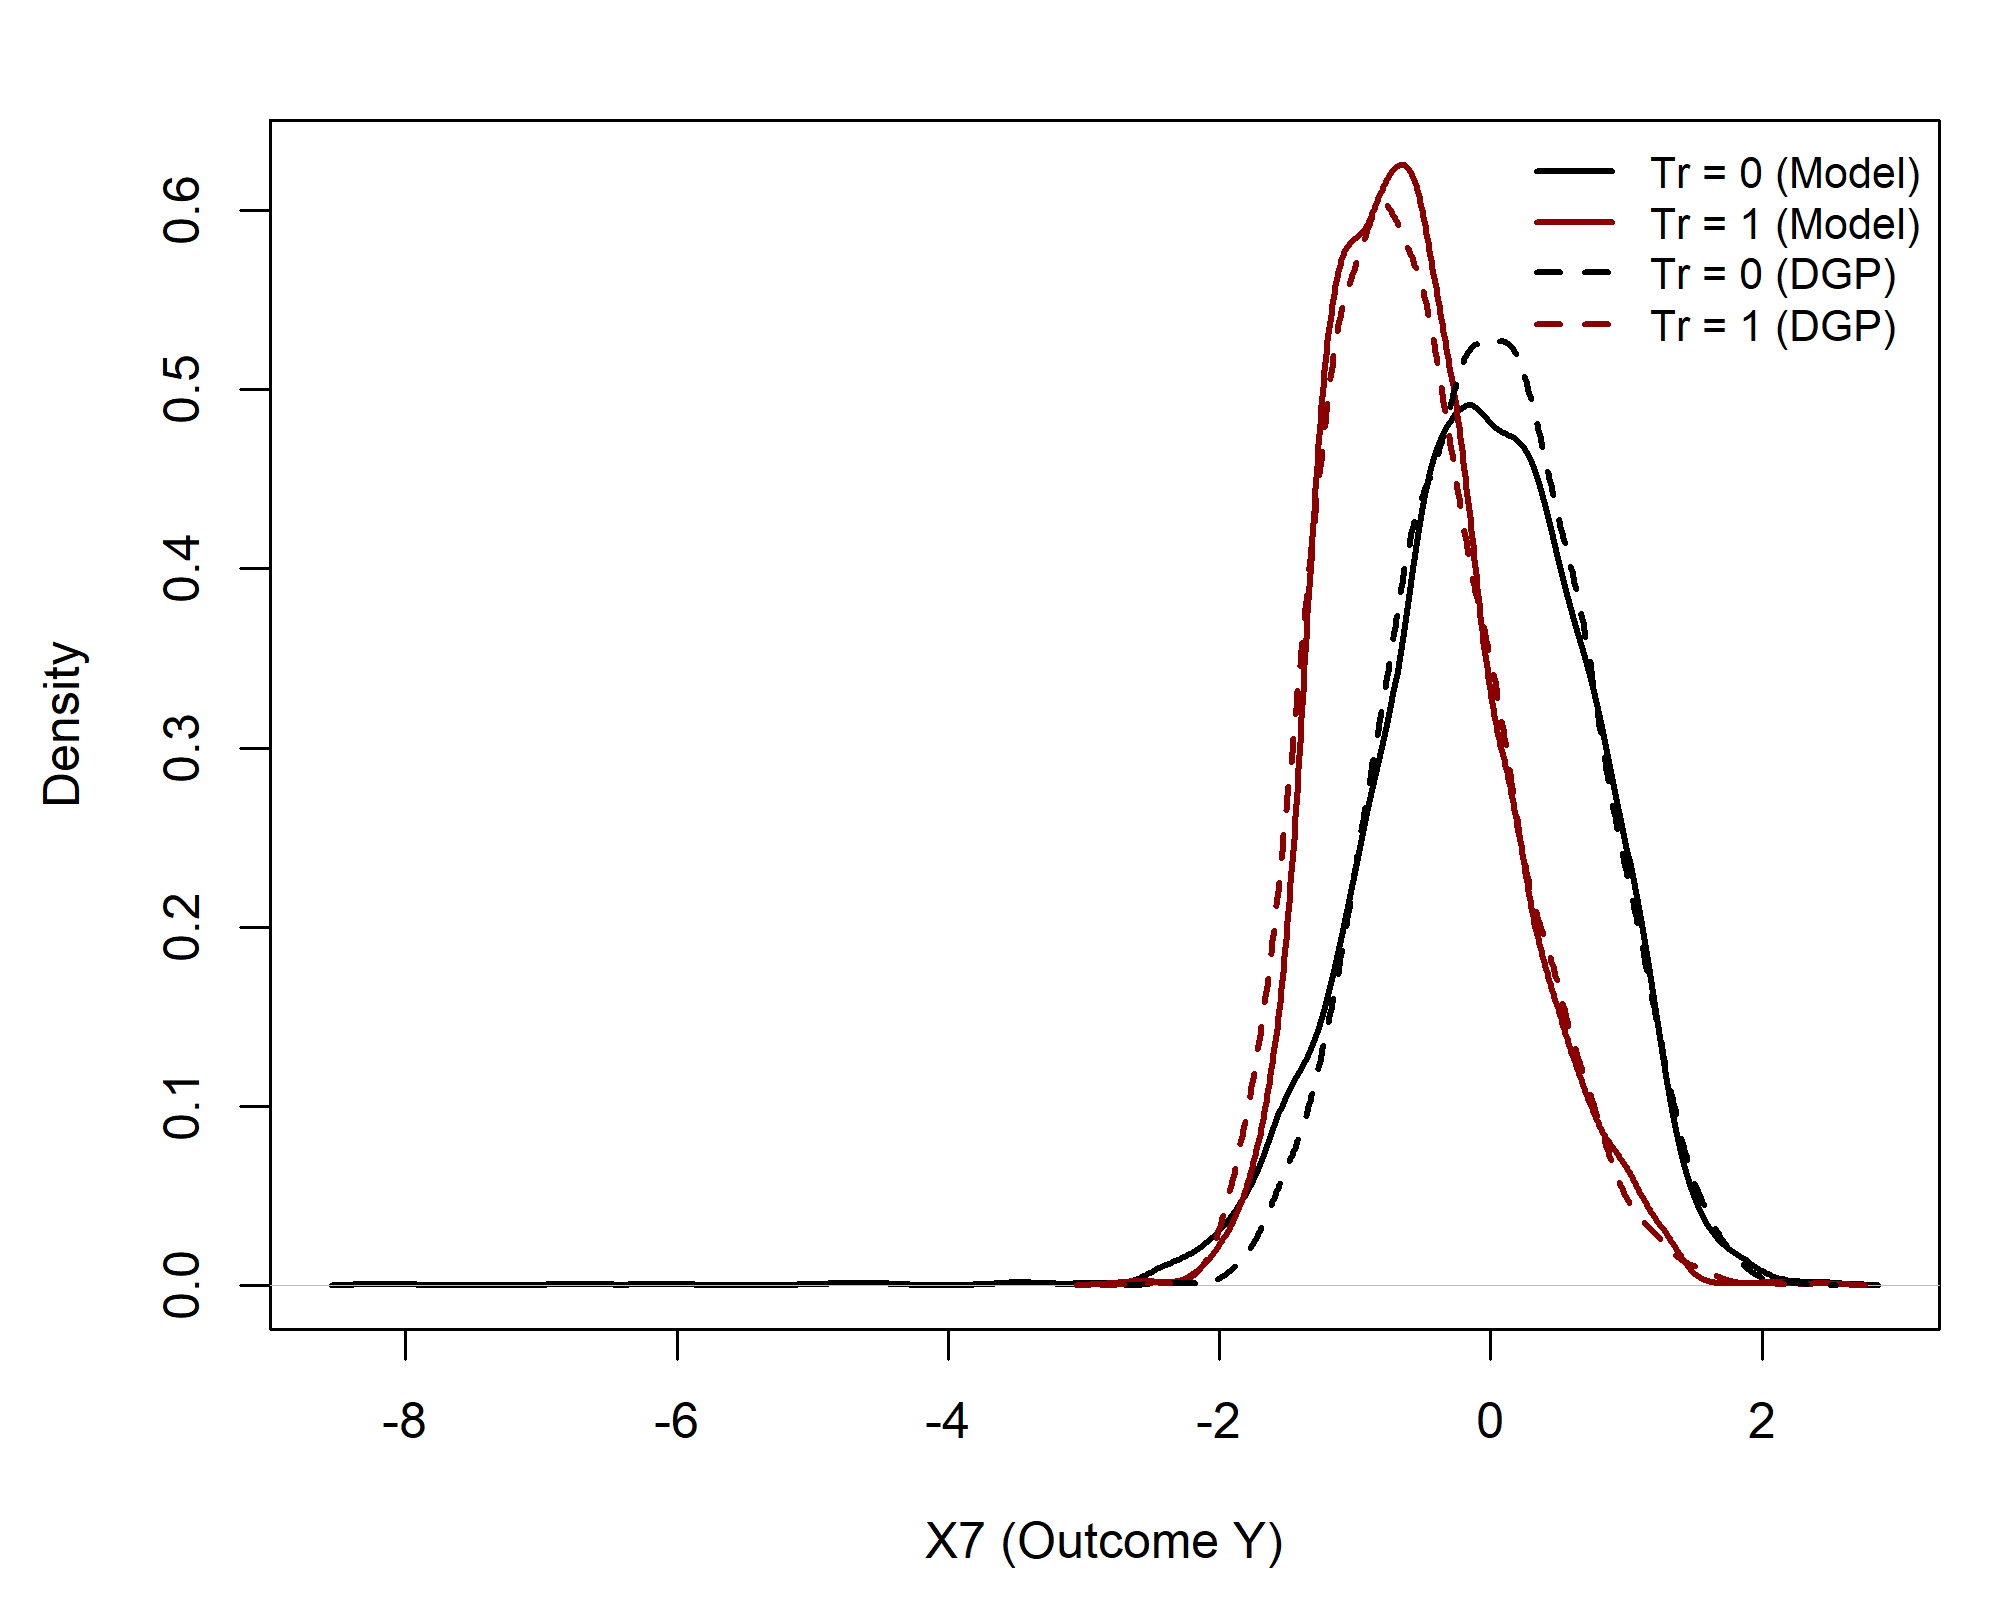
\includegraphics[width=0.45\textwidth]{img/results/rct_scenario2_X7_treatment_densities.png}
\caption{Distributions of the outcome variable ($X_7$) under treatment and control interventions for Scenario~(2), which includes a direct treatment effect but no interaction effects. This plot provides a higher-resolution view of the $X_7$ panels under do($X_4 = 0$) and do($X_4 = 1$) from Figure~\ref{fig:scenario2_sampling_distributions_vertical}. Left: Observational; Right: RCT setting.}
\label{fig:scenario2_outcome_distributions}
\end{figure}






\begin{figure}[htbp]
\centering
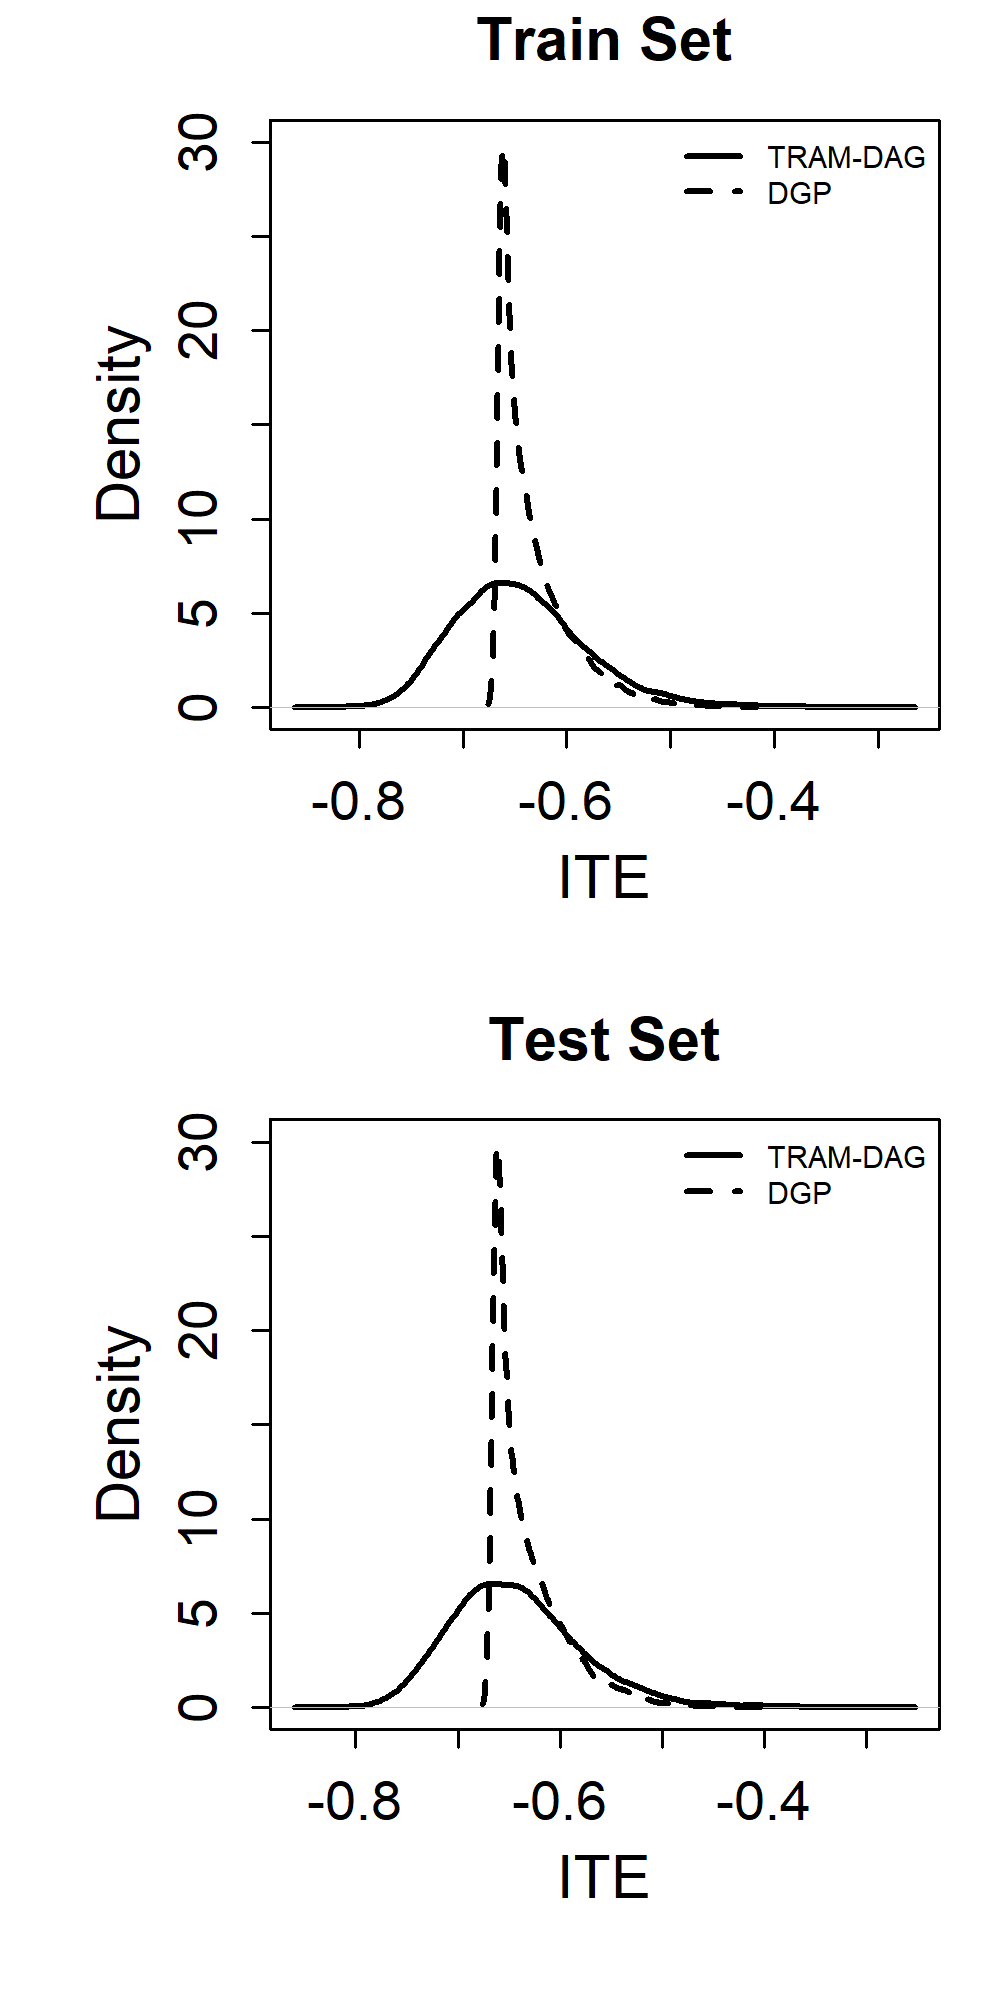
\includegraphics[width=0.33\textwidth]{img/results/observ_scenario2_ITE_densities_train_test.png}
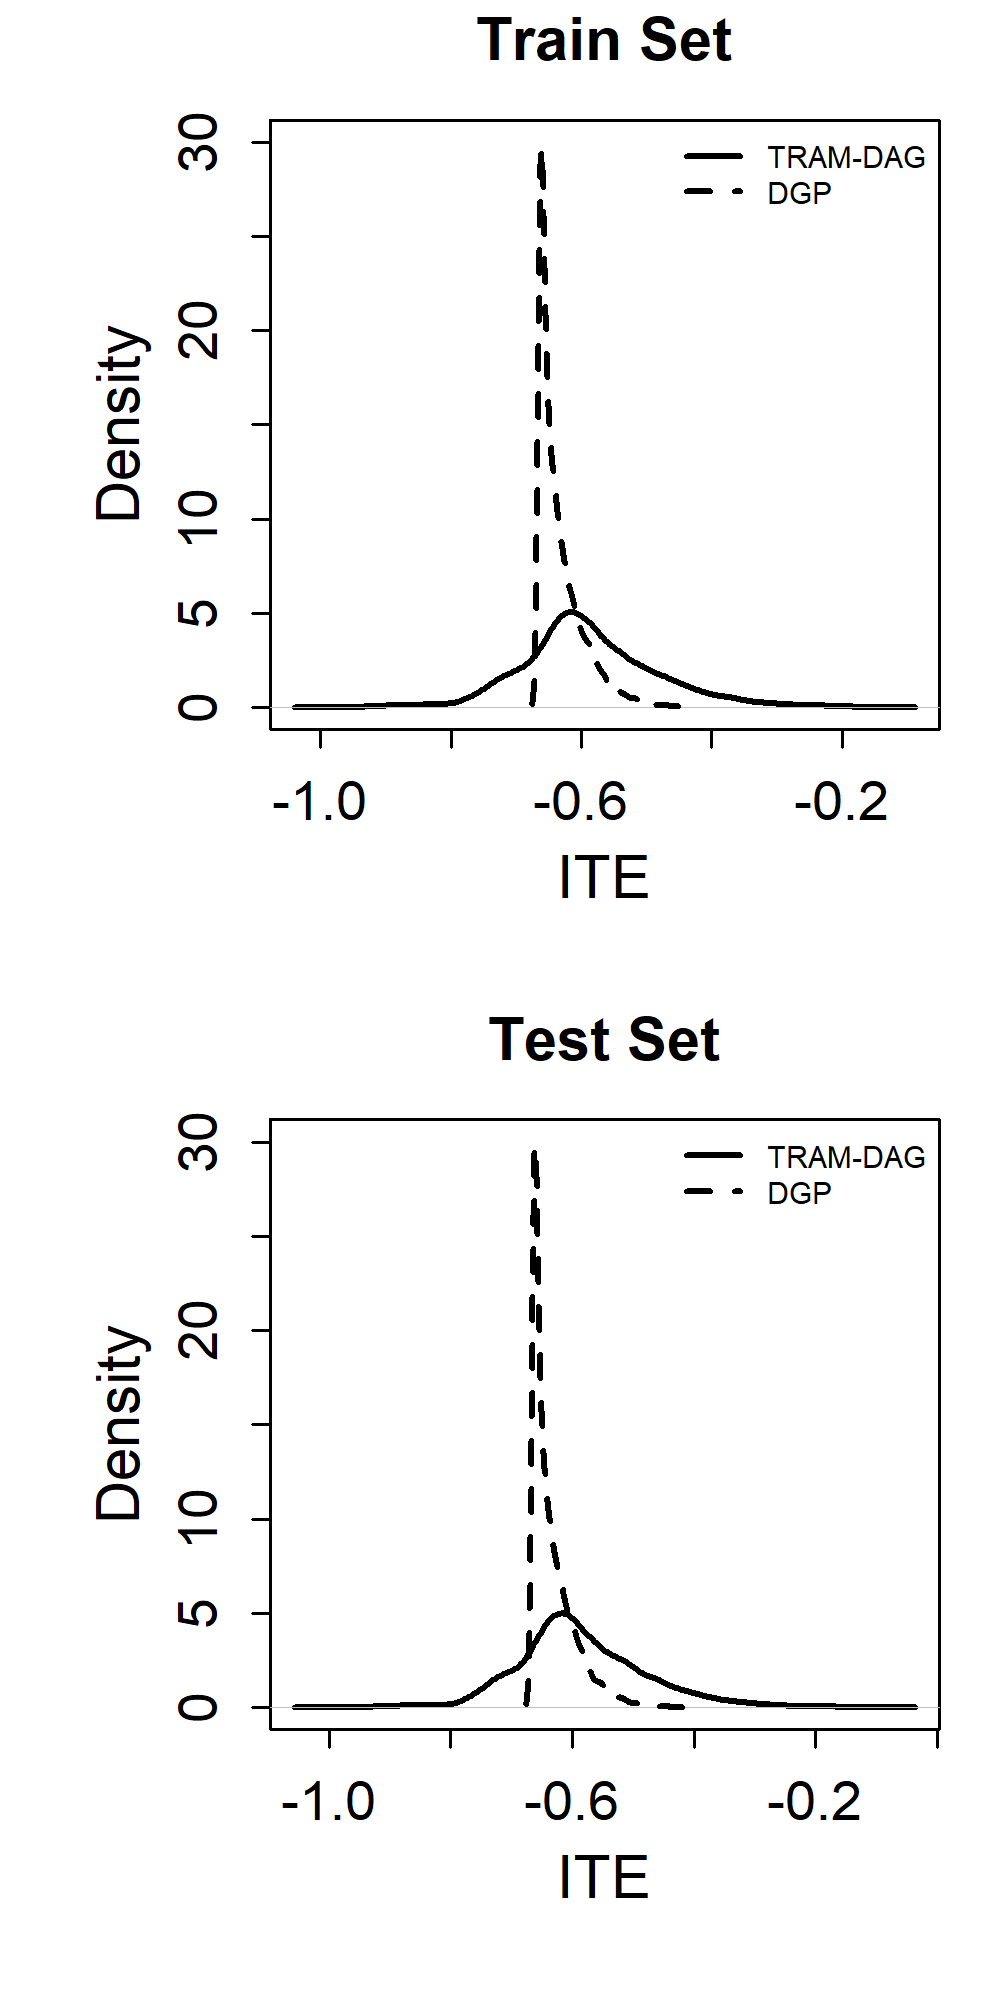
\includegraphics[width=0.33\textwidth]{img/results/rct_scenario2_ITE_densities_train_test.png}
\vspace{-17pt}
\caption{Densities of estimated ITEs compared to the true ITEs in the training and test datasets for Scenario~(2), which includes a direct treatment effect but no interaction effects. Left: Observational; Right: RCT setting.}
\label{fig:scenario2_ite_densities_train_test}
\end{figure}






\begin{figure}[htbp]
\centering
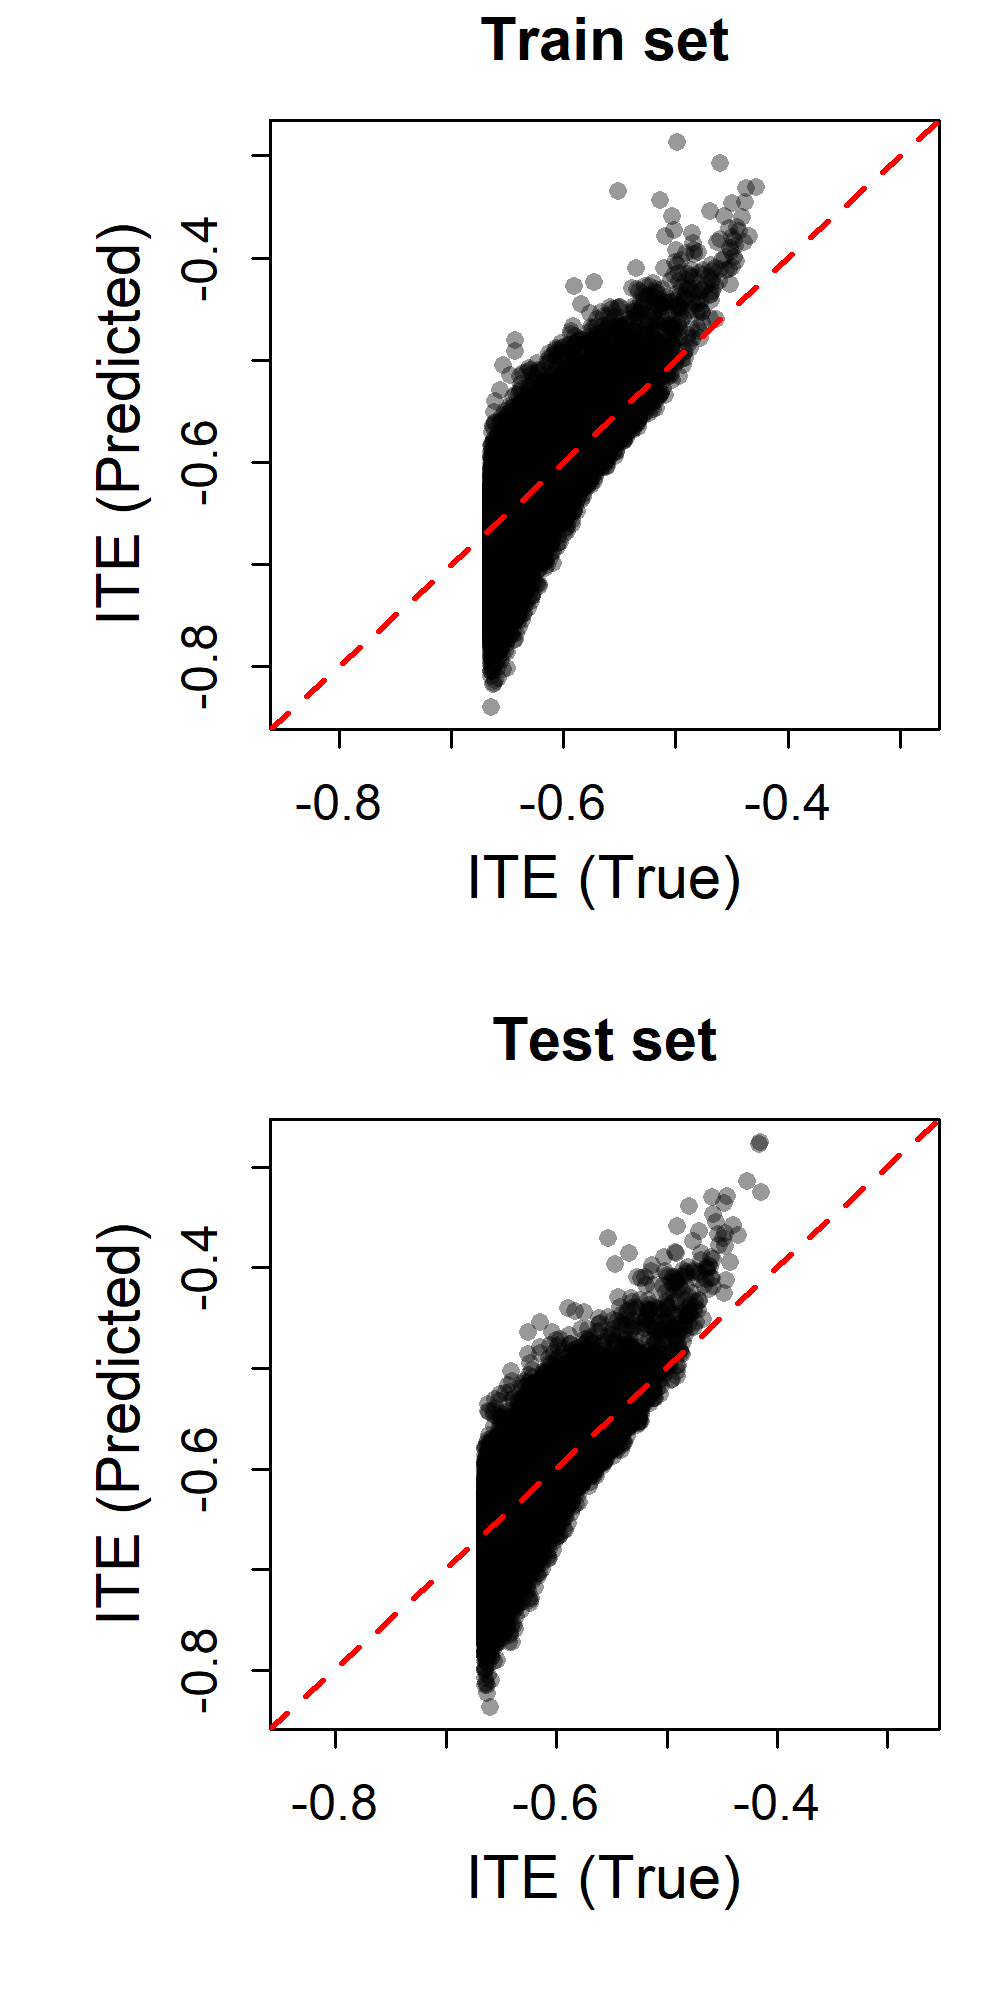
\includegraphics[width=0.33\textwidth]{img/results/observ_scenario2_ITE_scatter_train_test.png}
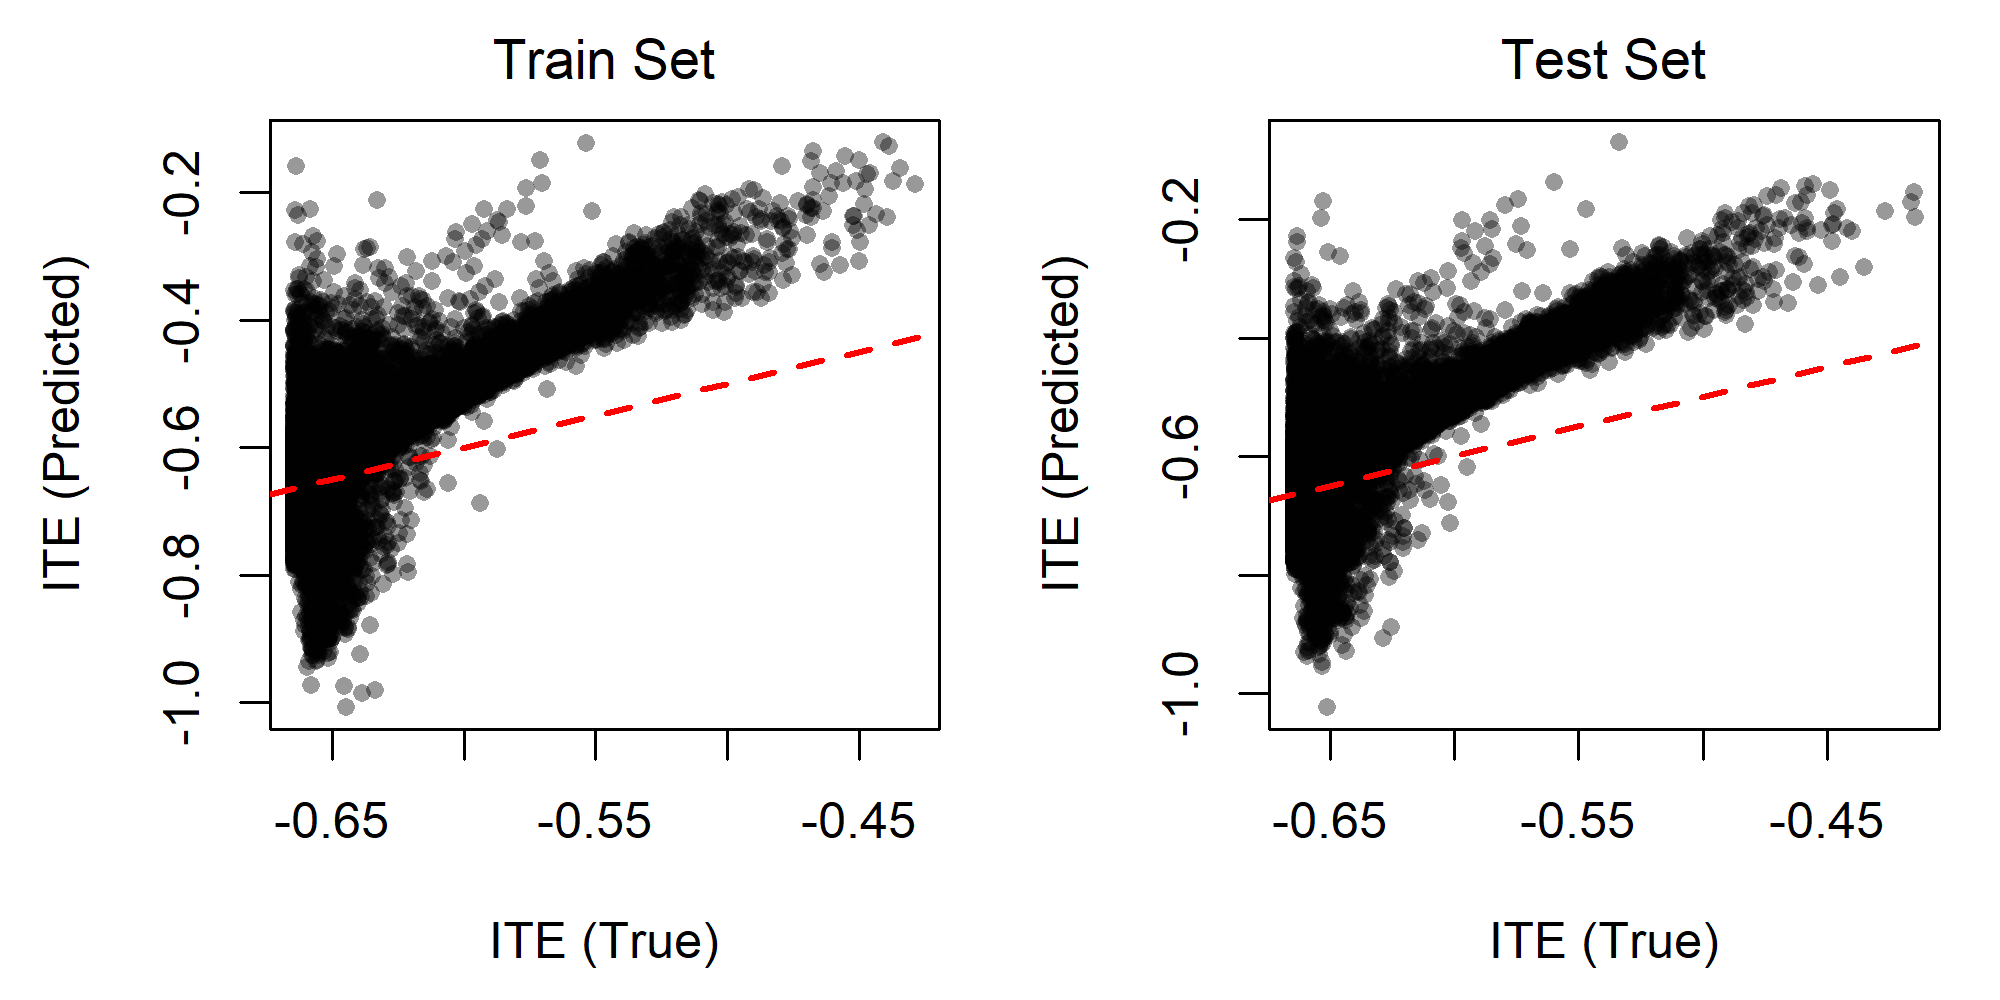
\includegraphics[width=0.33\textwidth]{img/results/rct_scenario2_ITE_scatter_train_test.png}
\vspace{-17pt}
\caption{Scatterplots of estimated ITEs compared to the true ITEs in the training and test datasets for Scenario~(2), which includes a direct treatment effect but no interaction effects. Left: Observational; Right: RCT setting.}
\label{fig:scenario2_ite_scatter_train_test}
\end{figure}




\begin{figure}[htbp]
\centering
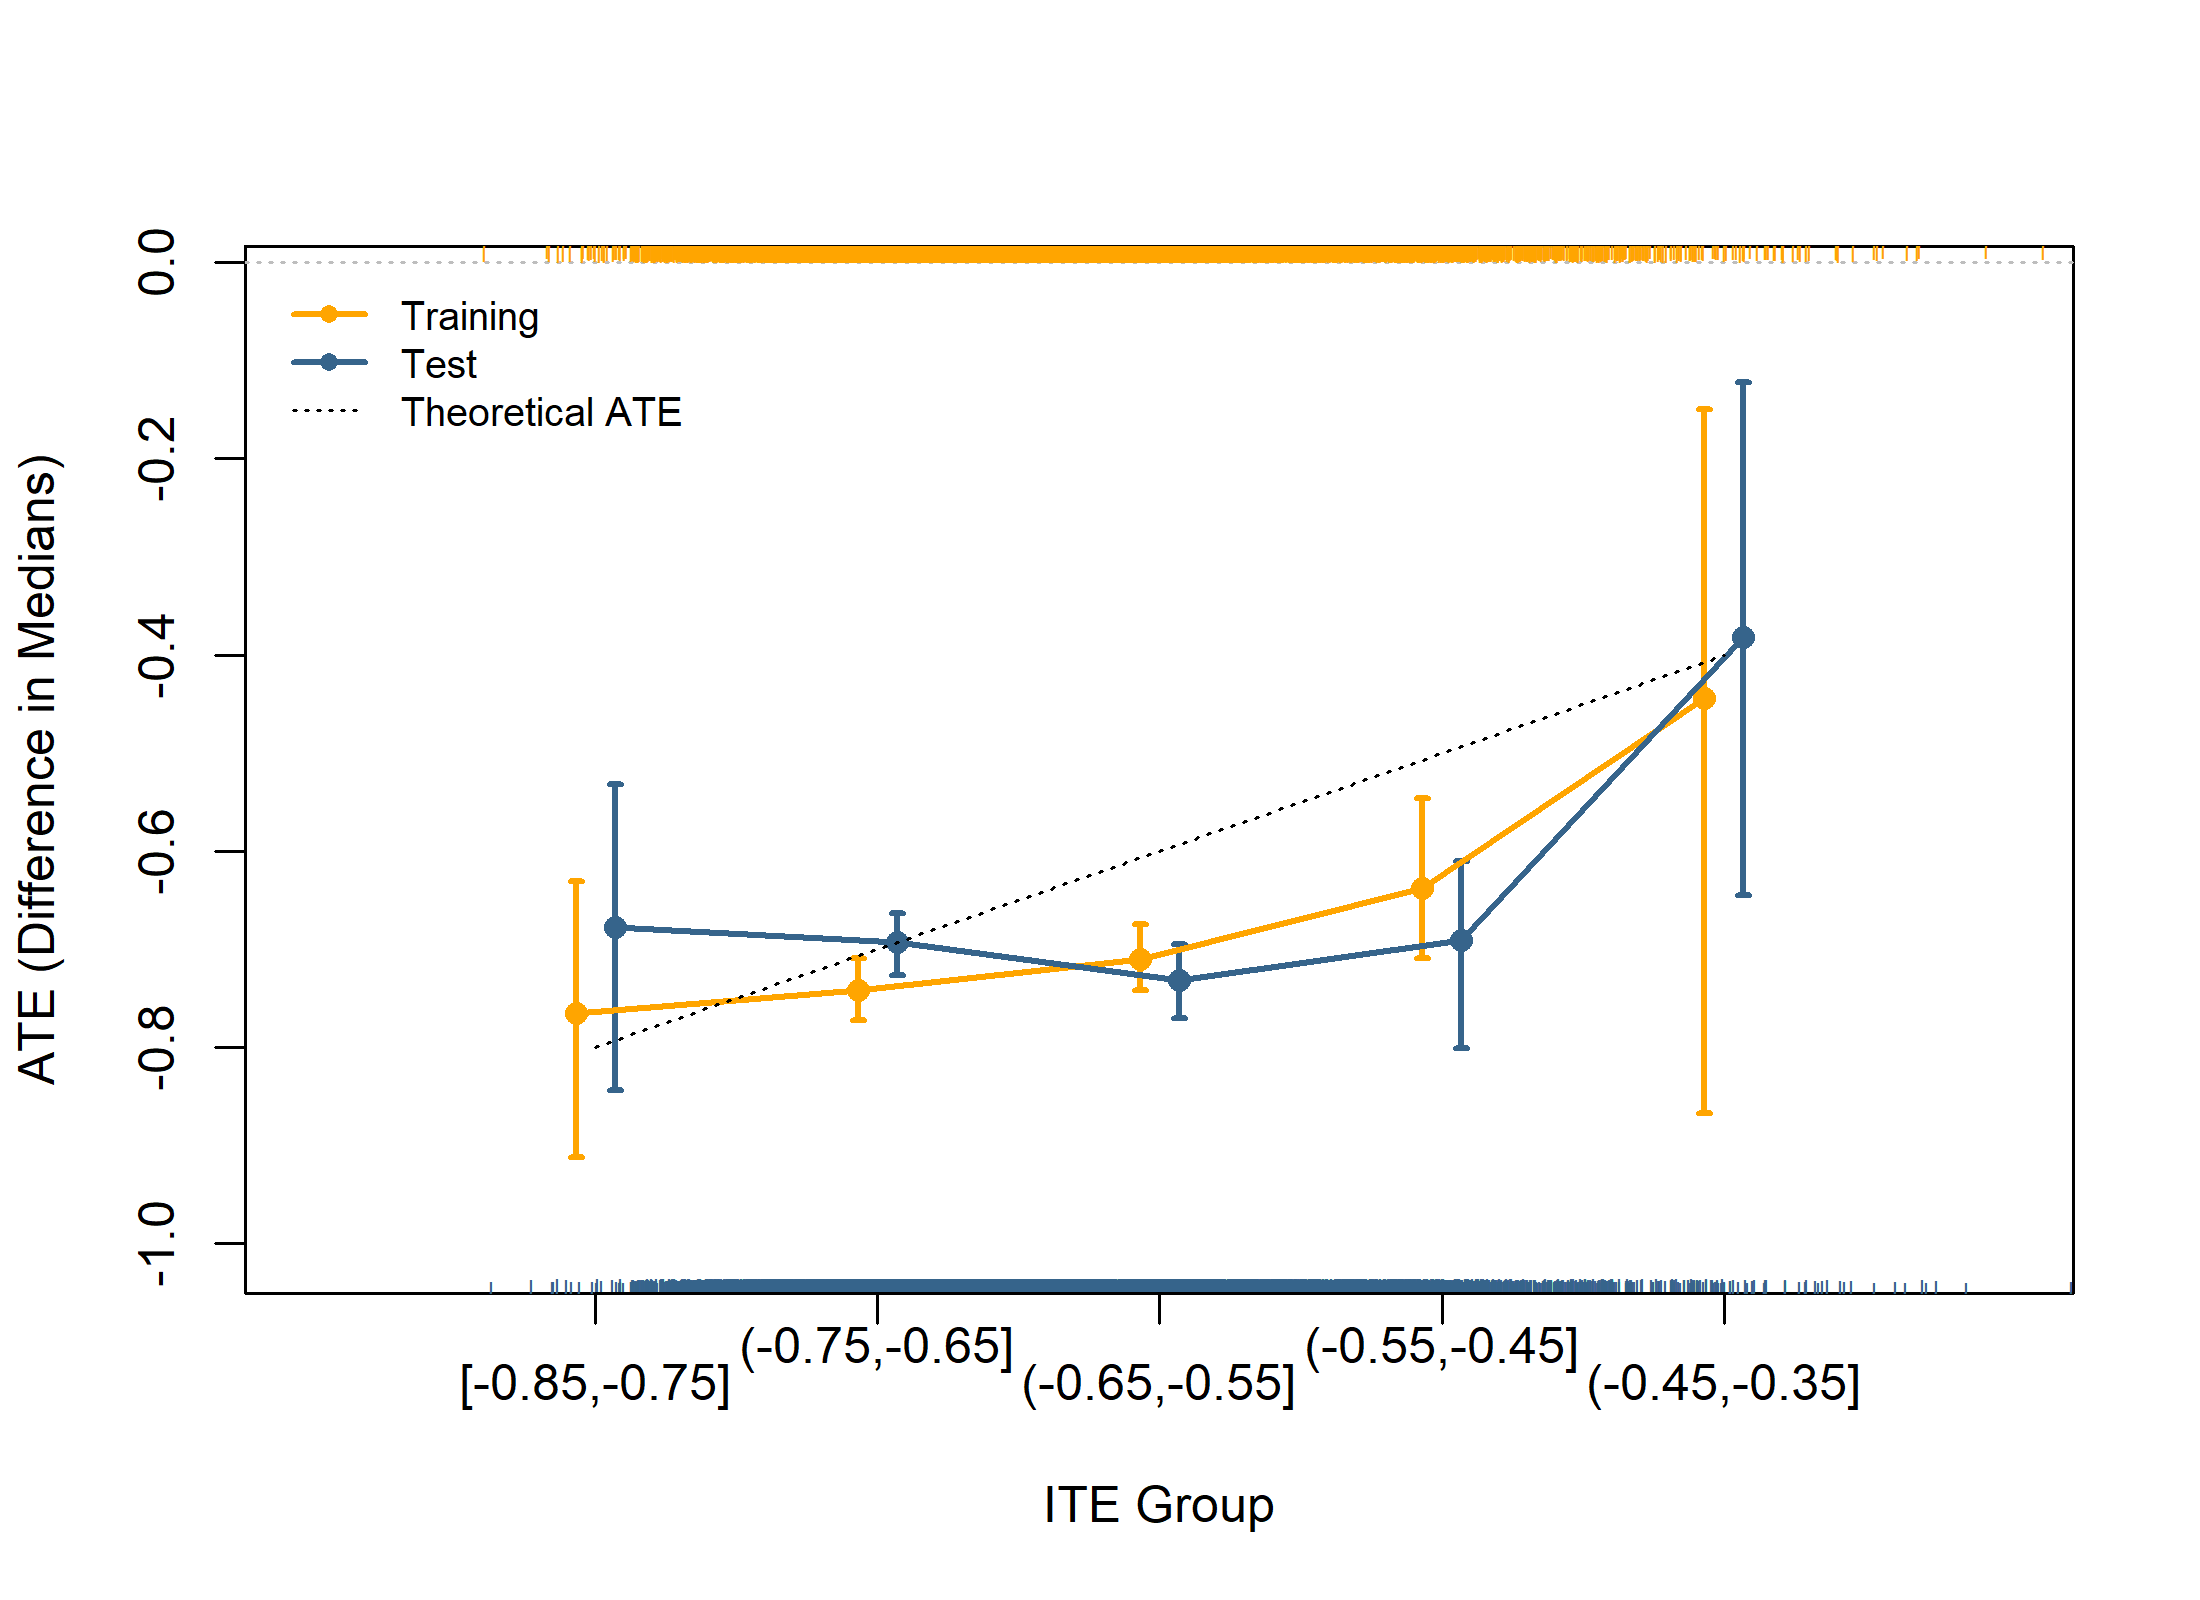
\includegraphics[width=0.8\textwidth]{img/results/observ_scenario2_ITE_ATE.png}
\vspace{-15pt}
\caption{ITE-ATE plot for Scenario~(2) in the observational setting, which includes a direct treatment effect but no interaction effects. Individuals are grouped into bins based on their estimated ITEs, and in each bin, the ATE is computed as the difference in medians of the observed outcomes under treatment and control. The 95\% bootstrap confidence intervals indicate uncertainty.}
\label{fig:observ_scenario2_ite_ATE}
\end{figure}



\begin{figure}[htbp]
\centering
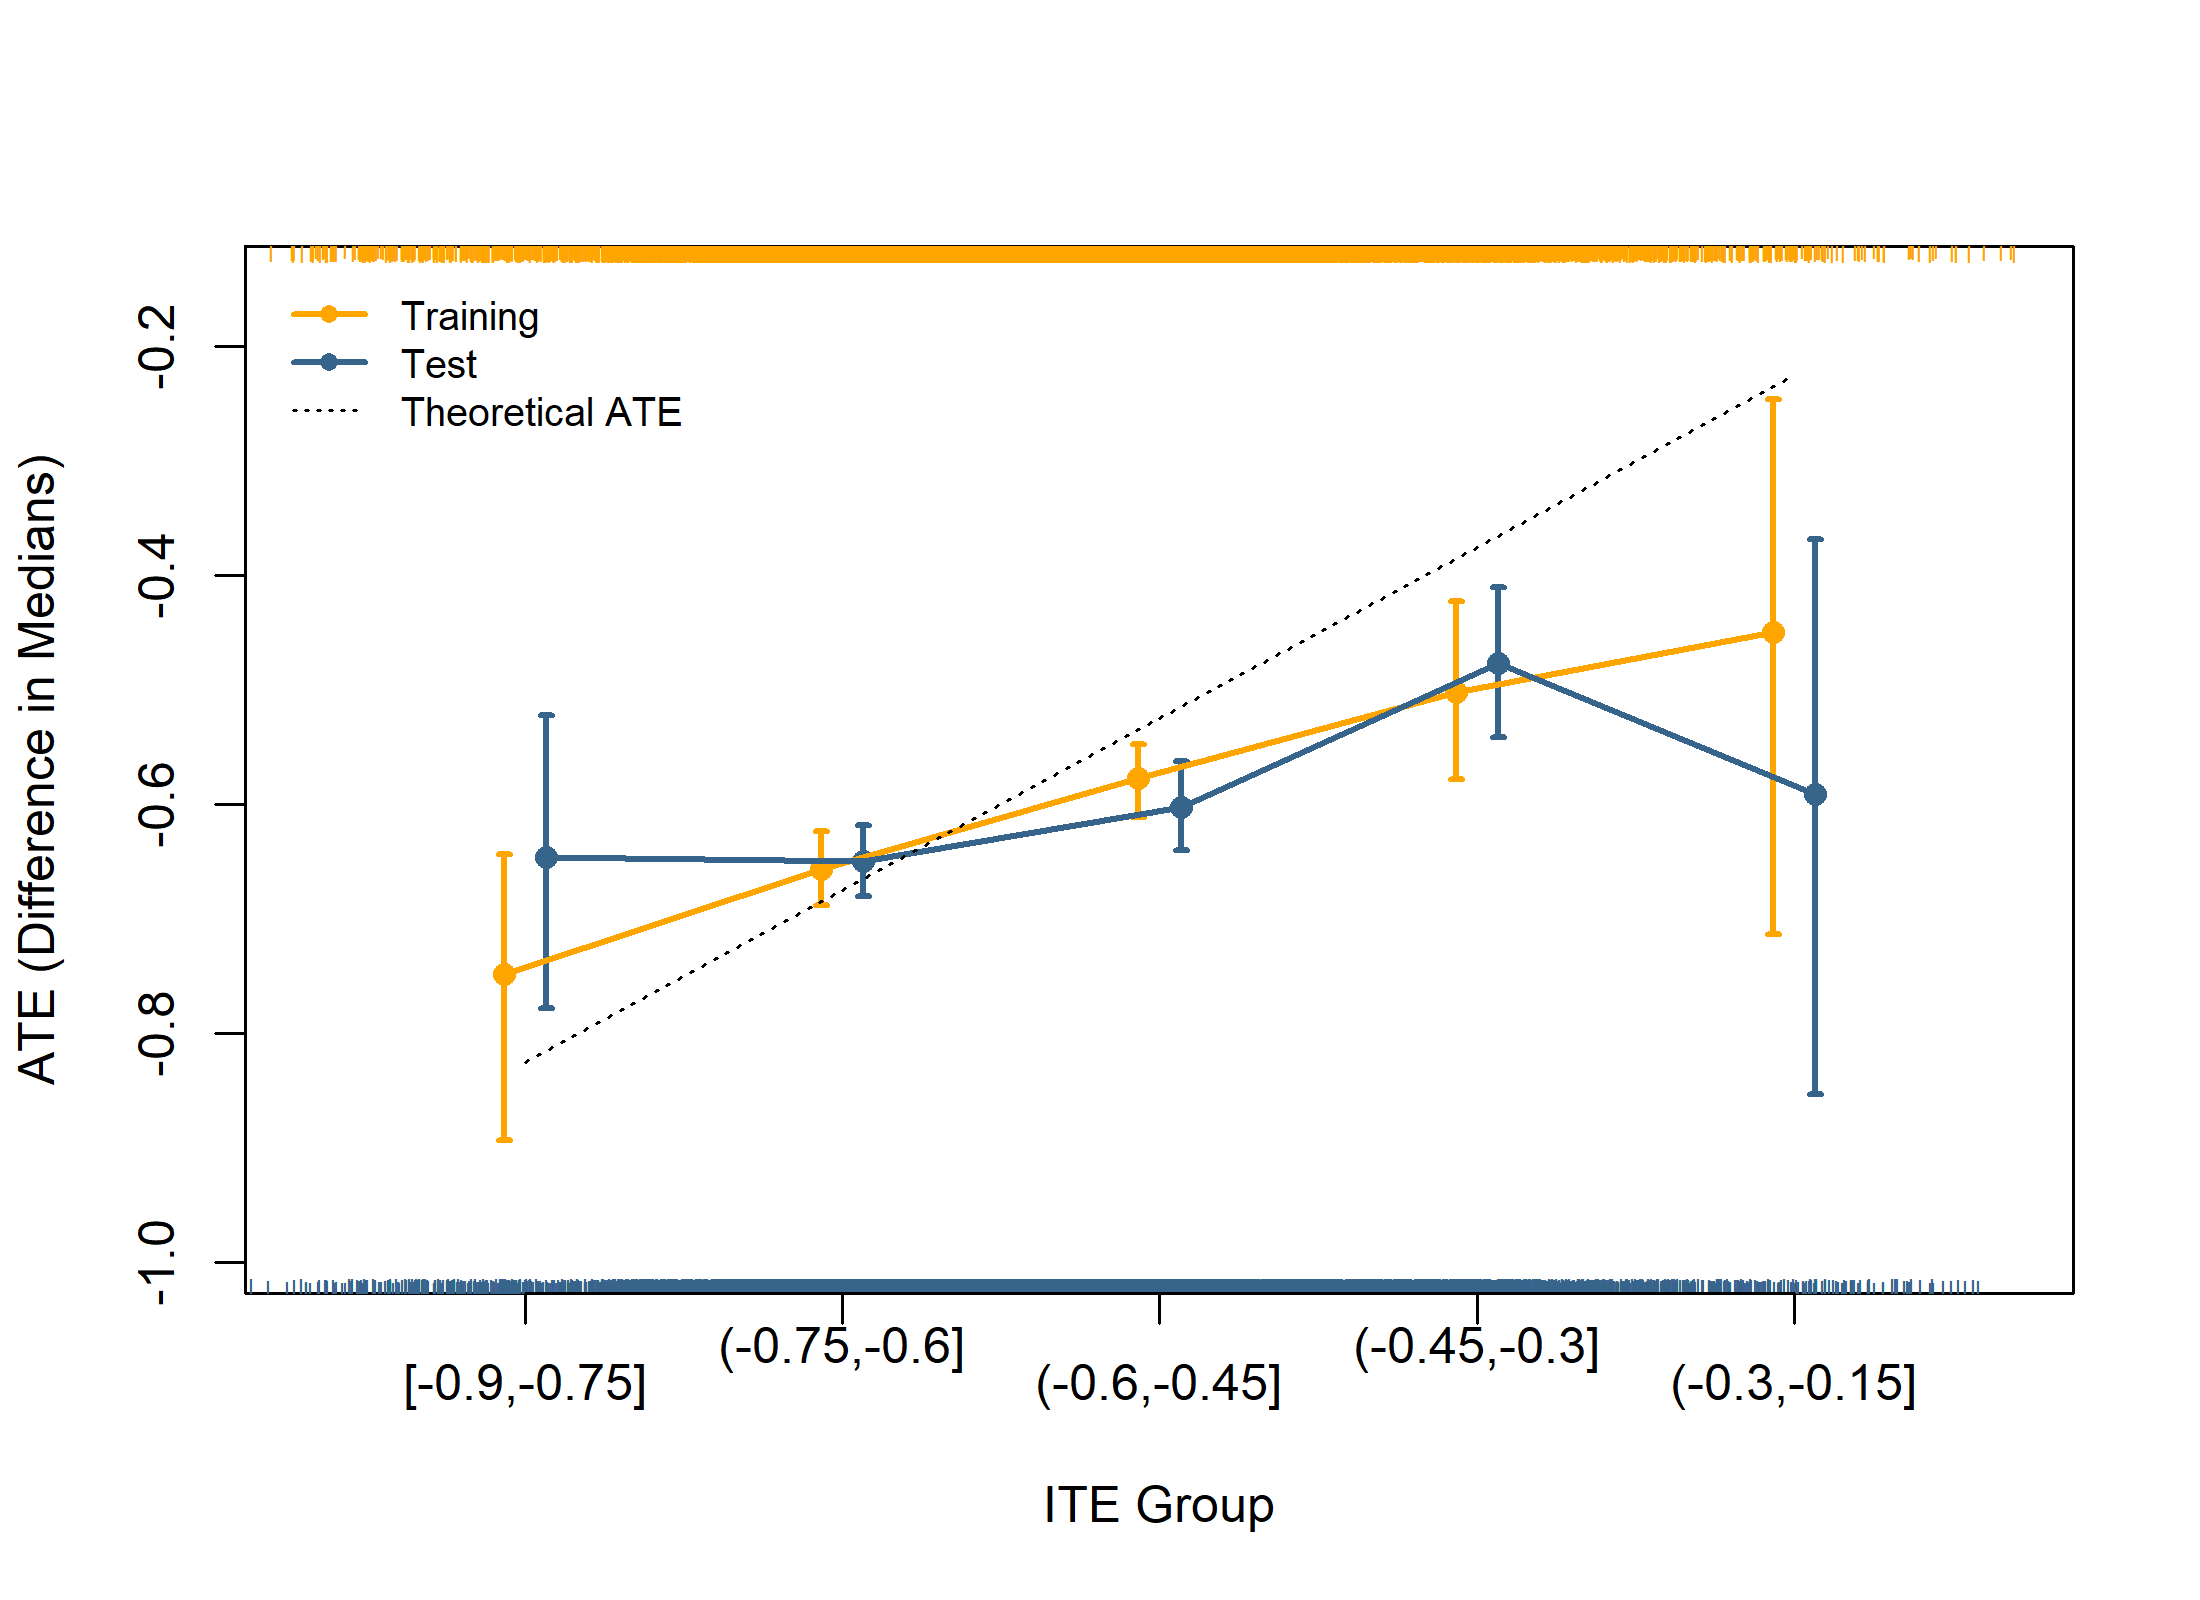
\includegraphics[width=0.8\textwidth]{img/results/rct_scenario2_ITE_ATE.png}
\vspace{-15pt}
\caption{ITE-ATE plot for Scenario~(2) in the RCT setting, which includes a direct treatment effect but no interaction effects. Individuals are grouped into bins based on their estimated ITEs, and in each bin, the ATE is computed as the difference in medians of the observed outcomes under treatment and control. The 95\% bootstrap confidence intervals indicate uncertainty.}
\label{fig:rct_scenario2_ite_ATE}
\end{figure}



\clearpage 



\subsection{Scenario (3): No direct effect, but with interaction effects}

\begin{figure}[H]
\centering
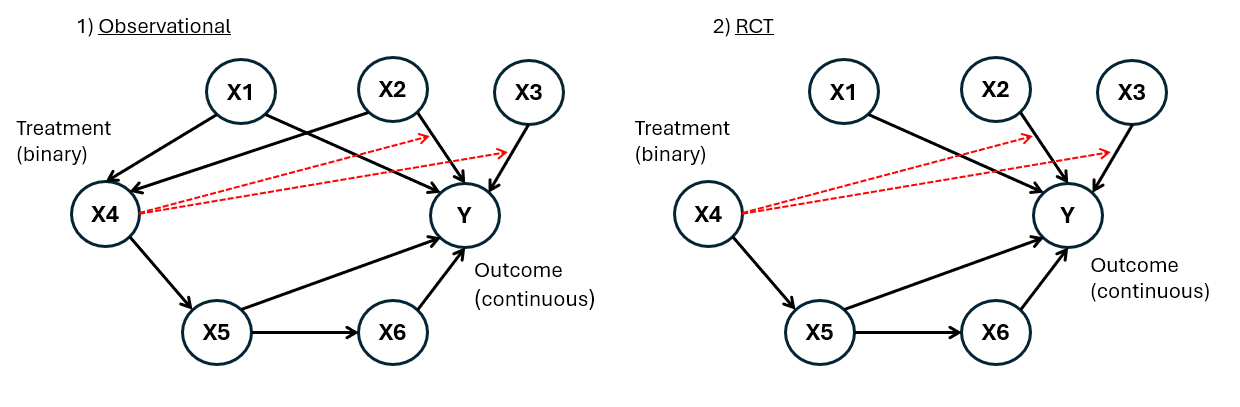
\includegraphics[width=0.85\textwidth]{img/exp4_dag_3.png}
\caption{DAGs for Scenario~(3), which includes no direct effect of the treatment on the outcome, but interaction effects with covariates $X_2$ and $X_3$. Left: Observational setting; Right: RCT setting.}
\label{fig:ite_dag_observational_3}
\end{figure}

Scenario~(3) includes no direct effect of the treatment on the outcome, but does include interaction effects between the treatment and covariates $X_2$ and $X_3$. Compared to Scenario~(1), removing the direct effect results in a more centered ITE distribution, as shown in Figure~\ref{fig:scenario3_ite_distribution_dgp}. In the test set of the RCT setting, the ATE measured as the difference in means was -0.048, with a 95\% confidence interval from -0.068 to -0.028.




\begin{table}[htbp]
\centering
\small
\caption{Scenario (3), without a direct treatment effect but including interaction effects: Comparison of ATE measures across train and test sets for the observational and RCT setting. $\text{Y}_\text{observed}^{(\text{Tr})}$ denotes the observed outcome under the treatment ($\text{Tr}$) actually received. The estimated ATE from $\text{mean}(\text{ITE}_\text{estimated})$ can be directly compared to the true $\text{mean}(\text{ITE}_\text{true})$, whereas comparisons to the empirical ATEs based on outcome differences should be interpreted with caution.}
\label{tab:scenario3_ate_comparison}
\begin{tabular}{l c c c c}
\toprule
\textbf{Measure} & \multicolumn{2}{c}{\textbf{Observational}} & \multicolumn{2}{c}{\textbf{RCT}} \\
\cmidrule(lr){2-3} \cmidrule(lr){4-5}
 & \textbf{Train} & \textbf{Test} & \textbf{Train} & \textbf{Test} \\
\midrule
ATE as $\text{mean}(\text{Y}_\text{observed}^{(1)}) - \text{mean}(\text{Y}_\text{observed}^{(0)})$ 
& NA & NA 
& -0.048 
& -0.048 \\

ATE as $\text{median}(\text{Y}_\text{observed}^{(1)}) - \text{median}(\text{Y}_\text{observed}^{(0)})$  
& NA & NA 
& -0.048 
& -0.059 \\

ATE as mean(ITE$_\text{true}$)  
& -0.065 
& -0.068 
& -0.065 
& -0.068 \\

ATE as mean(ITE$_\text{estimated}$) 
& -0.059 
& -0.061 
& -0.051 
& -0.053 \\
\bottomrule
\end{tabular}
\end{table}


% \begin{table}[htbp]
% \centering
% \small
% \caption{Scenario (3), without direct treatment effect but including interaction effects: Comparison of ATE measures across train and test sets for the observational and RCT setting.}
% \label{tab:scenario3_ate_comparison_old}
% \begin{tabular}{l c c c c}
% \toprule
% \textbf{Measure} & \multicolumn{2}{c}{\textbf{Observational}} & \multicolumn{2}{c}{\textbf{RCT}} \\
% \cmidrule(lr){2-3} \cmidrule(lr){4-5}
%  & \textbf{Train} & \textbf{Test} & \textbf{Train} & \textbf{Test} \\
% \midrule
% ATE as $\text{mean}(\text{Y}_\text{observed}^{(1)}) - \text{mean}(\text{Y}_\text{observed}^{(0)})$ & NA & NA & round(rct_scenario3$dev_ATE_observed_Y_mean_diff, 3) & round(rct_scenario3$val_ATE_observed_Y_mean_diff, 3) \\
% ATE as $\text{median}(\text{Y}_\text{observed}^{(1)}) - \text{median}(\text{Y}_\text{observed}^{(0)})$ & NA & NA & round(rct_scenario3$dev_ATE_observed_Y_median_diff, 3) & round(rct_scenario3$val_ATE_observed_Y_median_diff, 3) \\
% ATE as mean(ITE$_\text{true}$)  & round(observ_scenario3$dev_ITE_median_average, 3) & round(observ_scenario3$val_ITE_median_average, 3) & round(rct_scenario3$dev_ITE_median_average, 3) & round(rct_scenario3$val_ITE_median_average, 3) \\
% ATE as mean(ITE$_\text{estimated}$) & round(observ_scenario3$dev_ITE_median_pred_average, 3) & round(observ_scenario3$val_ITE_median_pred_average, 3) & round(rct_scenario3$dev_ITE_median_pred_average, 3) & round(rct_scenario3$val_ITE_median_pred_average, 3) \\
% \bottomrule
% \end{tabular}
% \end{table}
% 


\begin{figure}[htbp]
\centering
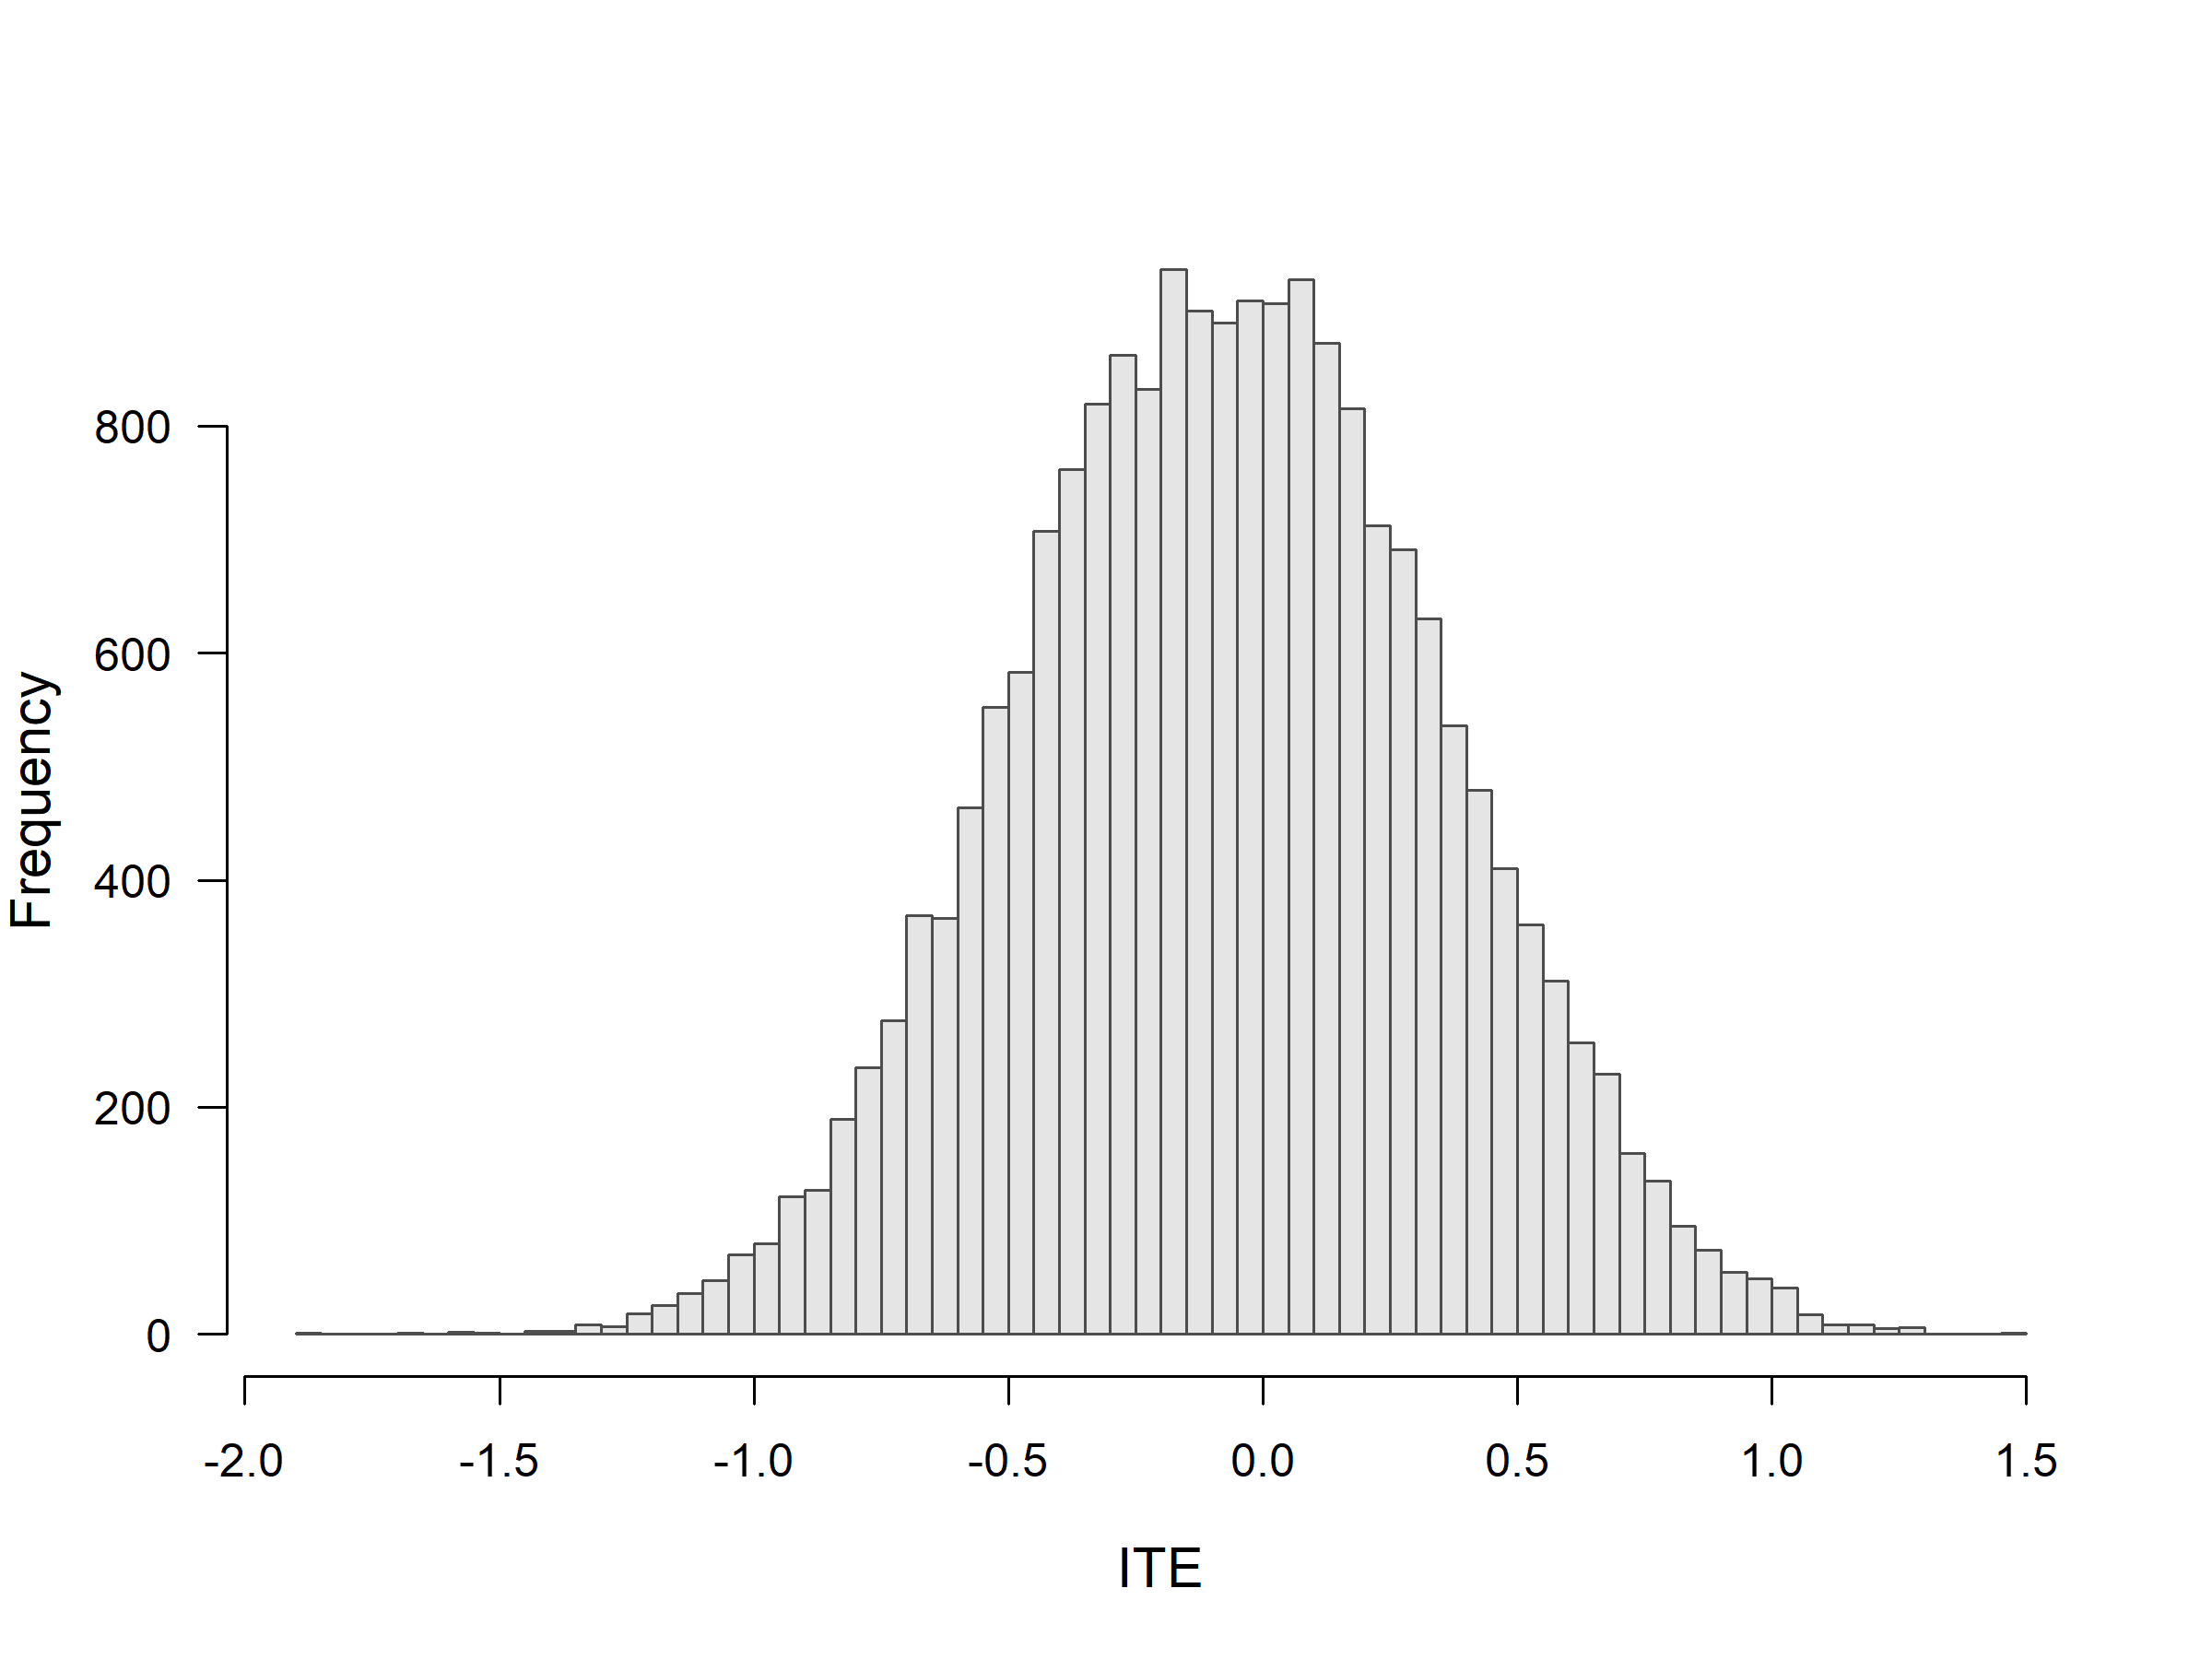
\includegraphics[width=0.7\textwidth]{img/results/observ_scenario3_ite_distribution_dgp.png}
\caption{True ITE distribution resulting from the DGP for Scenario~(3), which includes interaction effects but no direct treatment effect. The true ITEs are identical in the observational and RCT settings, since they are based on the potential outcomes under both treatment allocations. Left: Observational; Right: RCT setting.}
\label{fig:scenario3_ite_distribution_dgp}
\end{figure}



\begin{figure}[htbp]
\centering
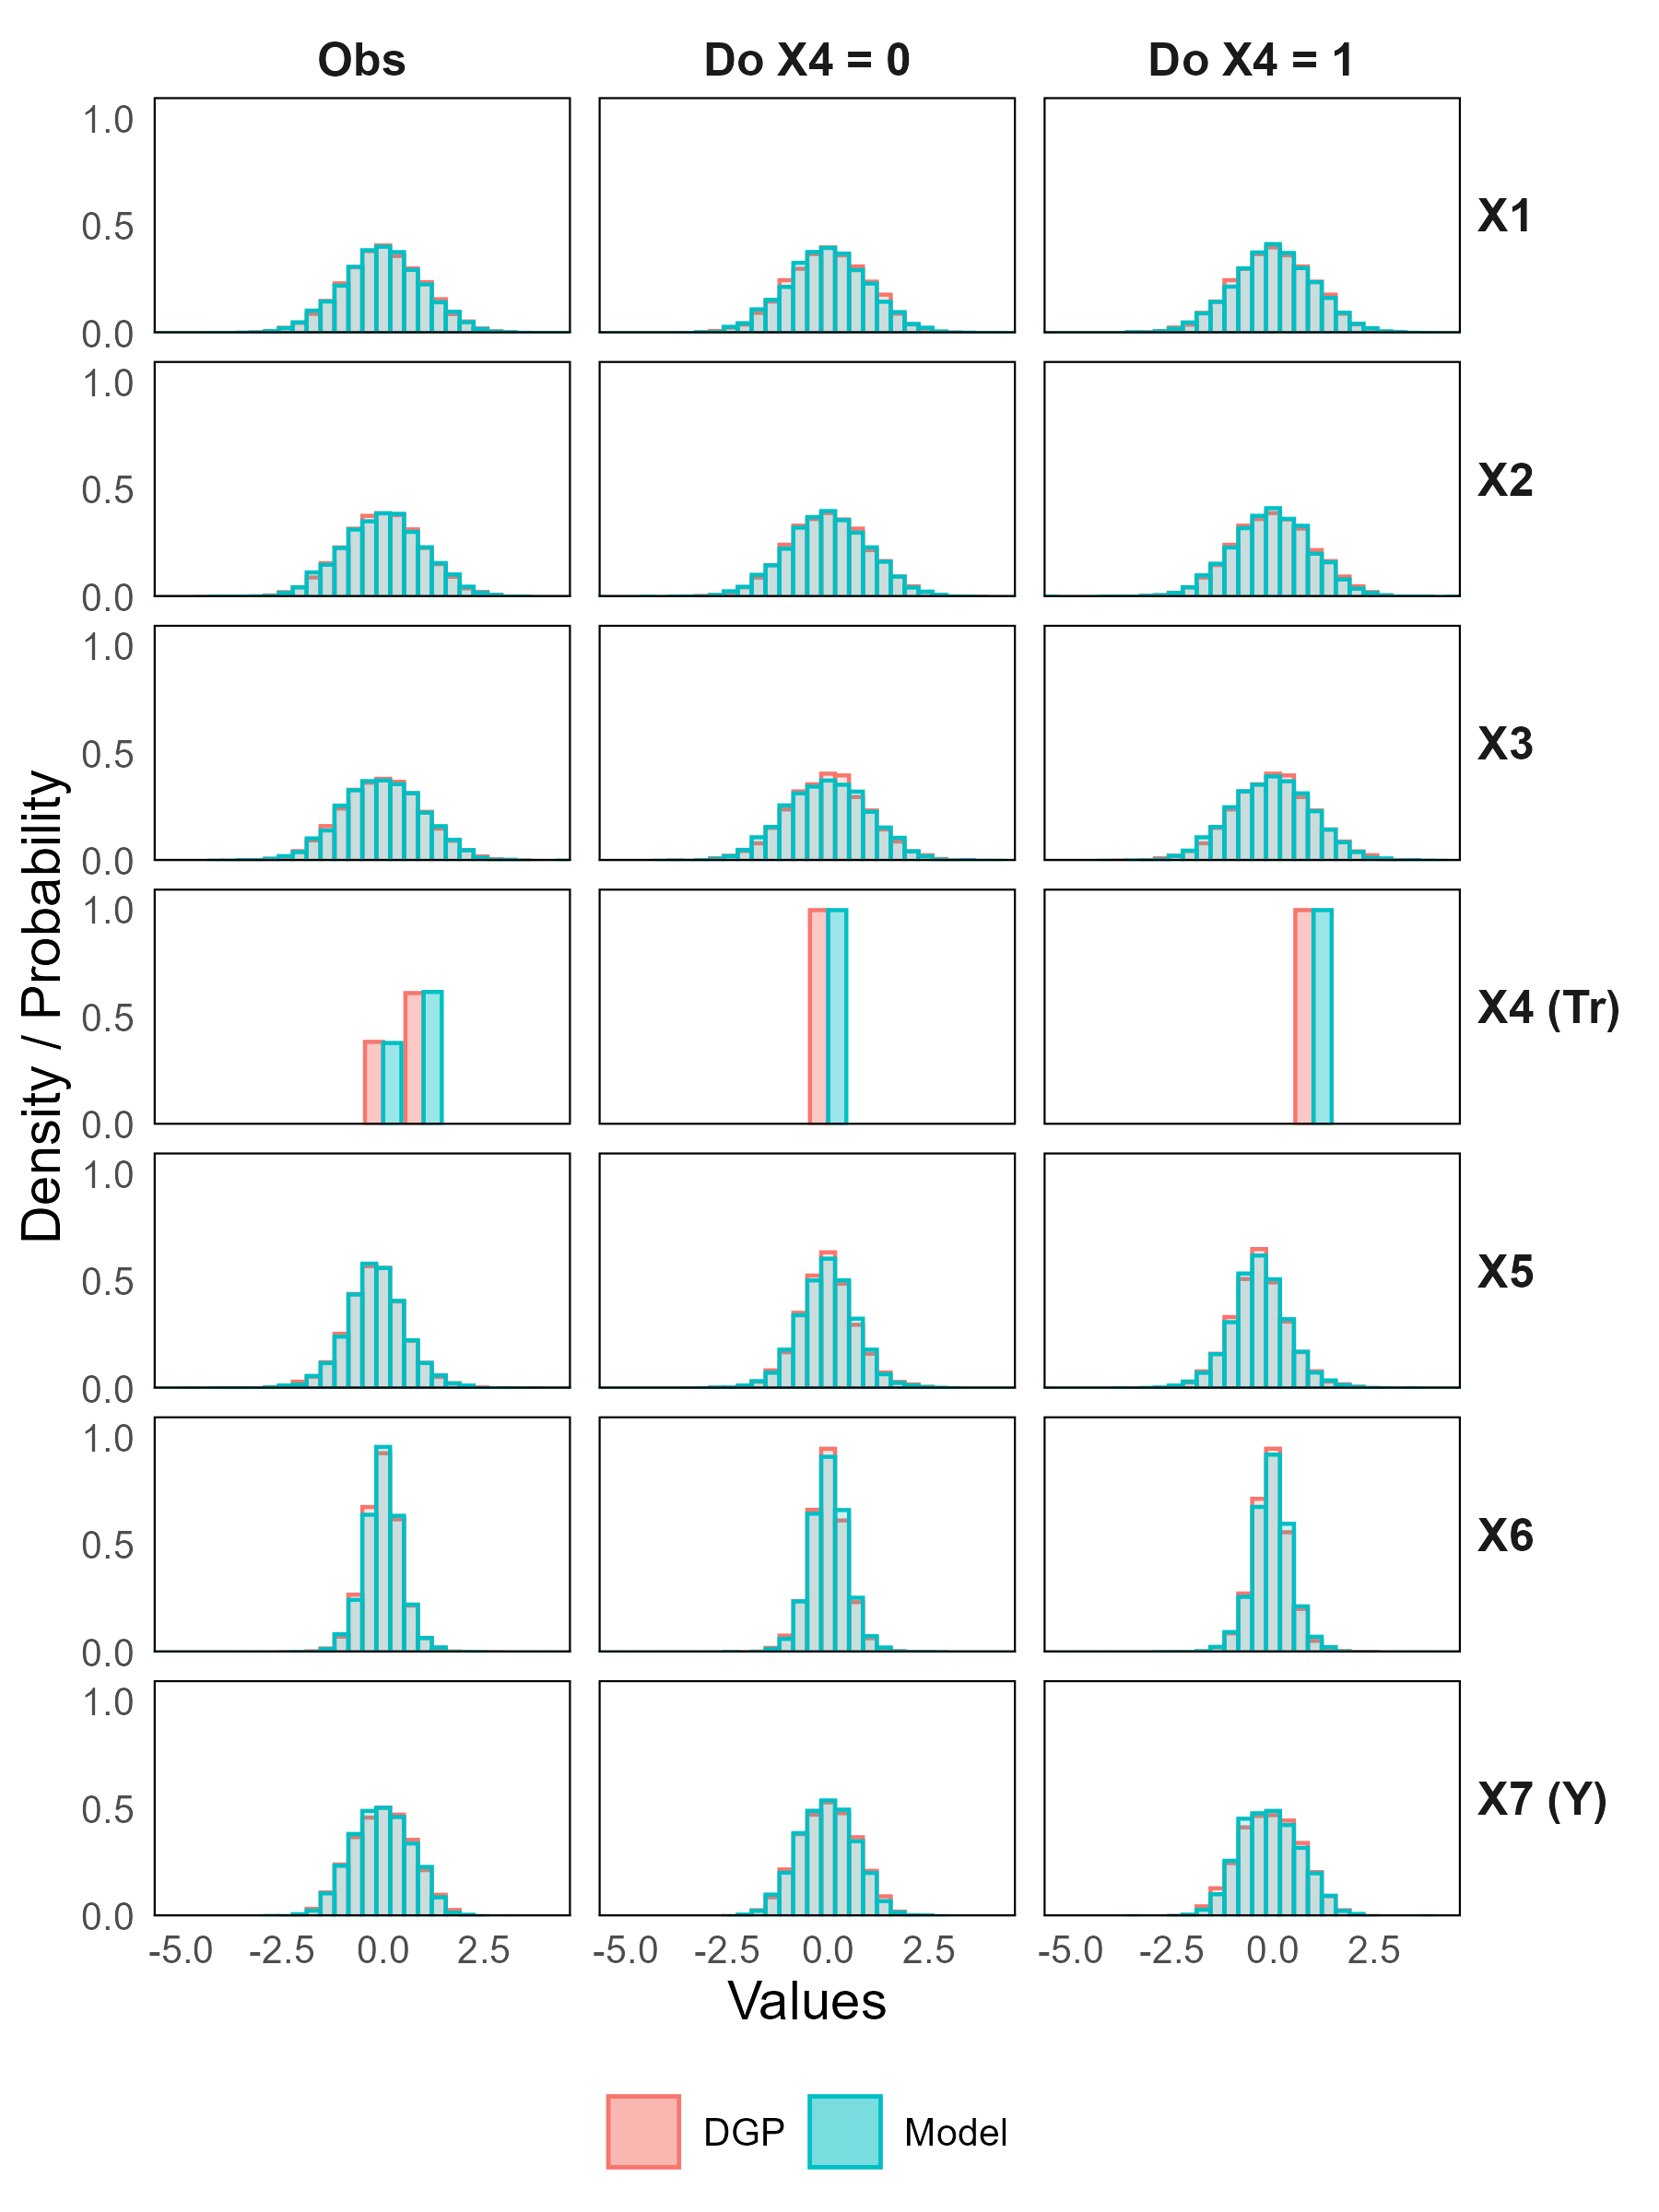
\includegraphics[width=0.45\textwidth]{img/results/observ_scenario3_sampling_distributions_vertical.png}
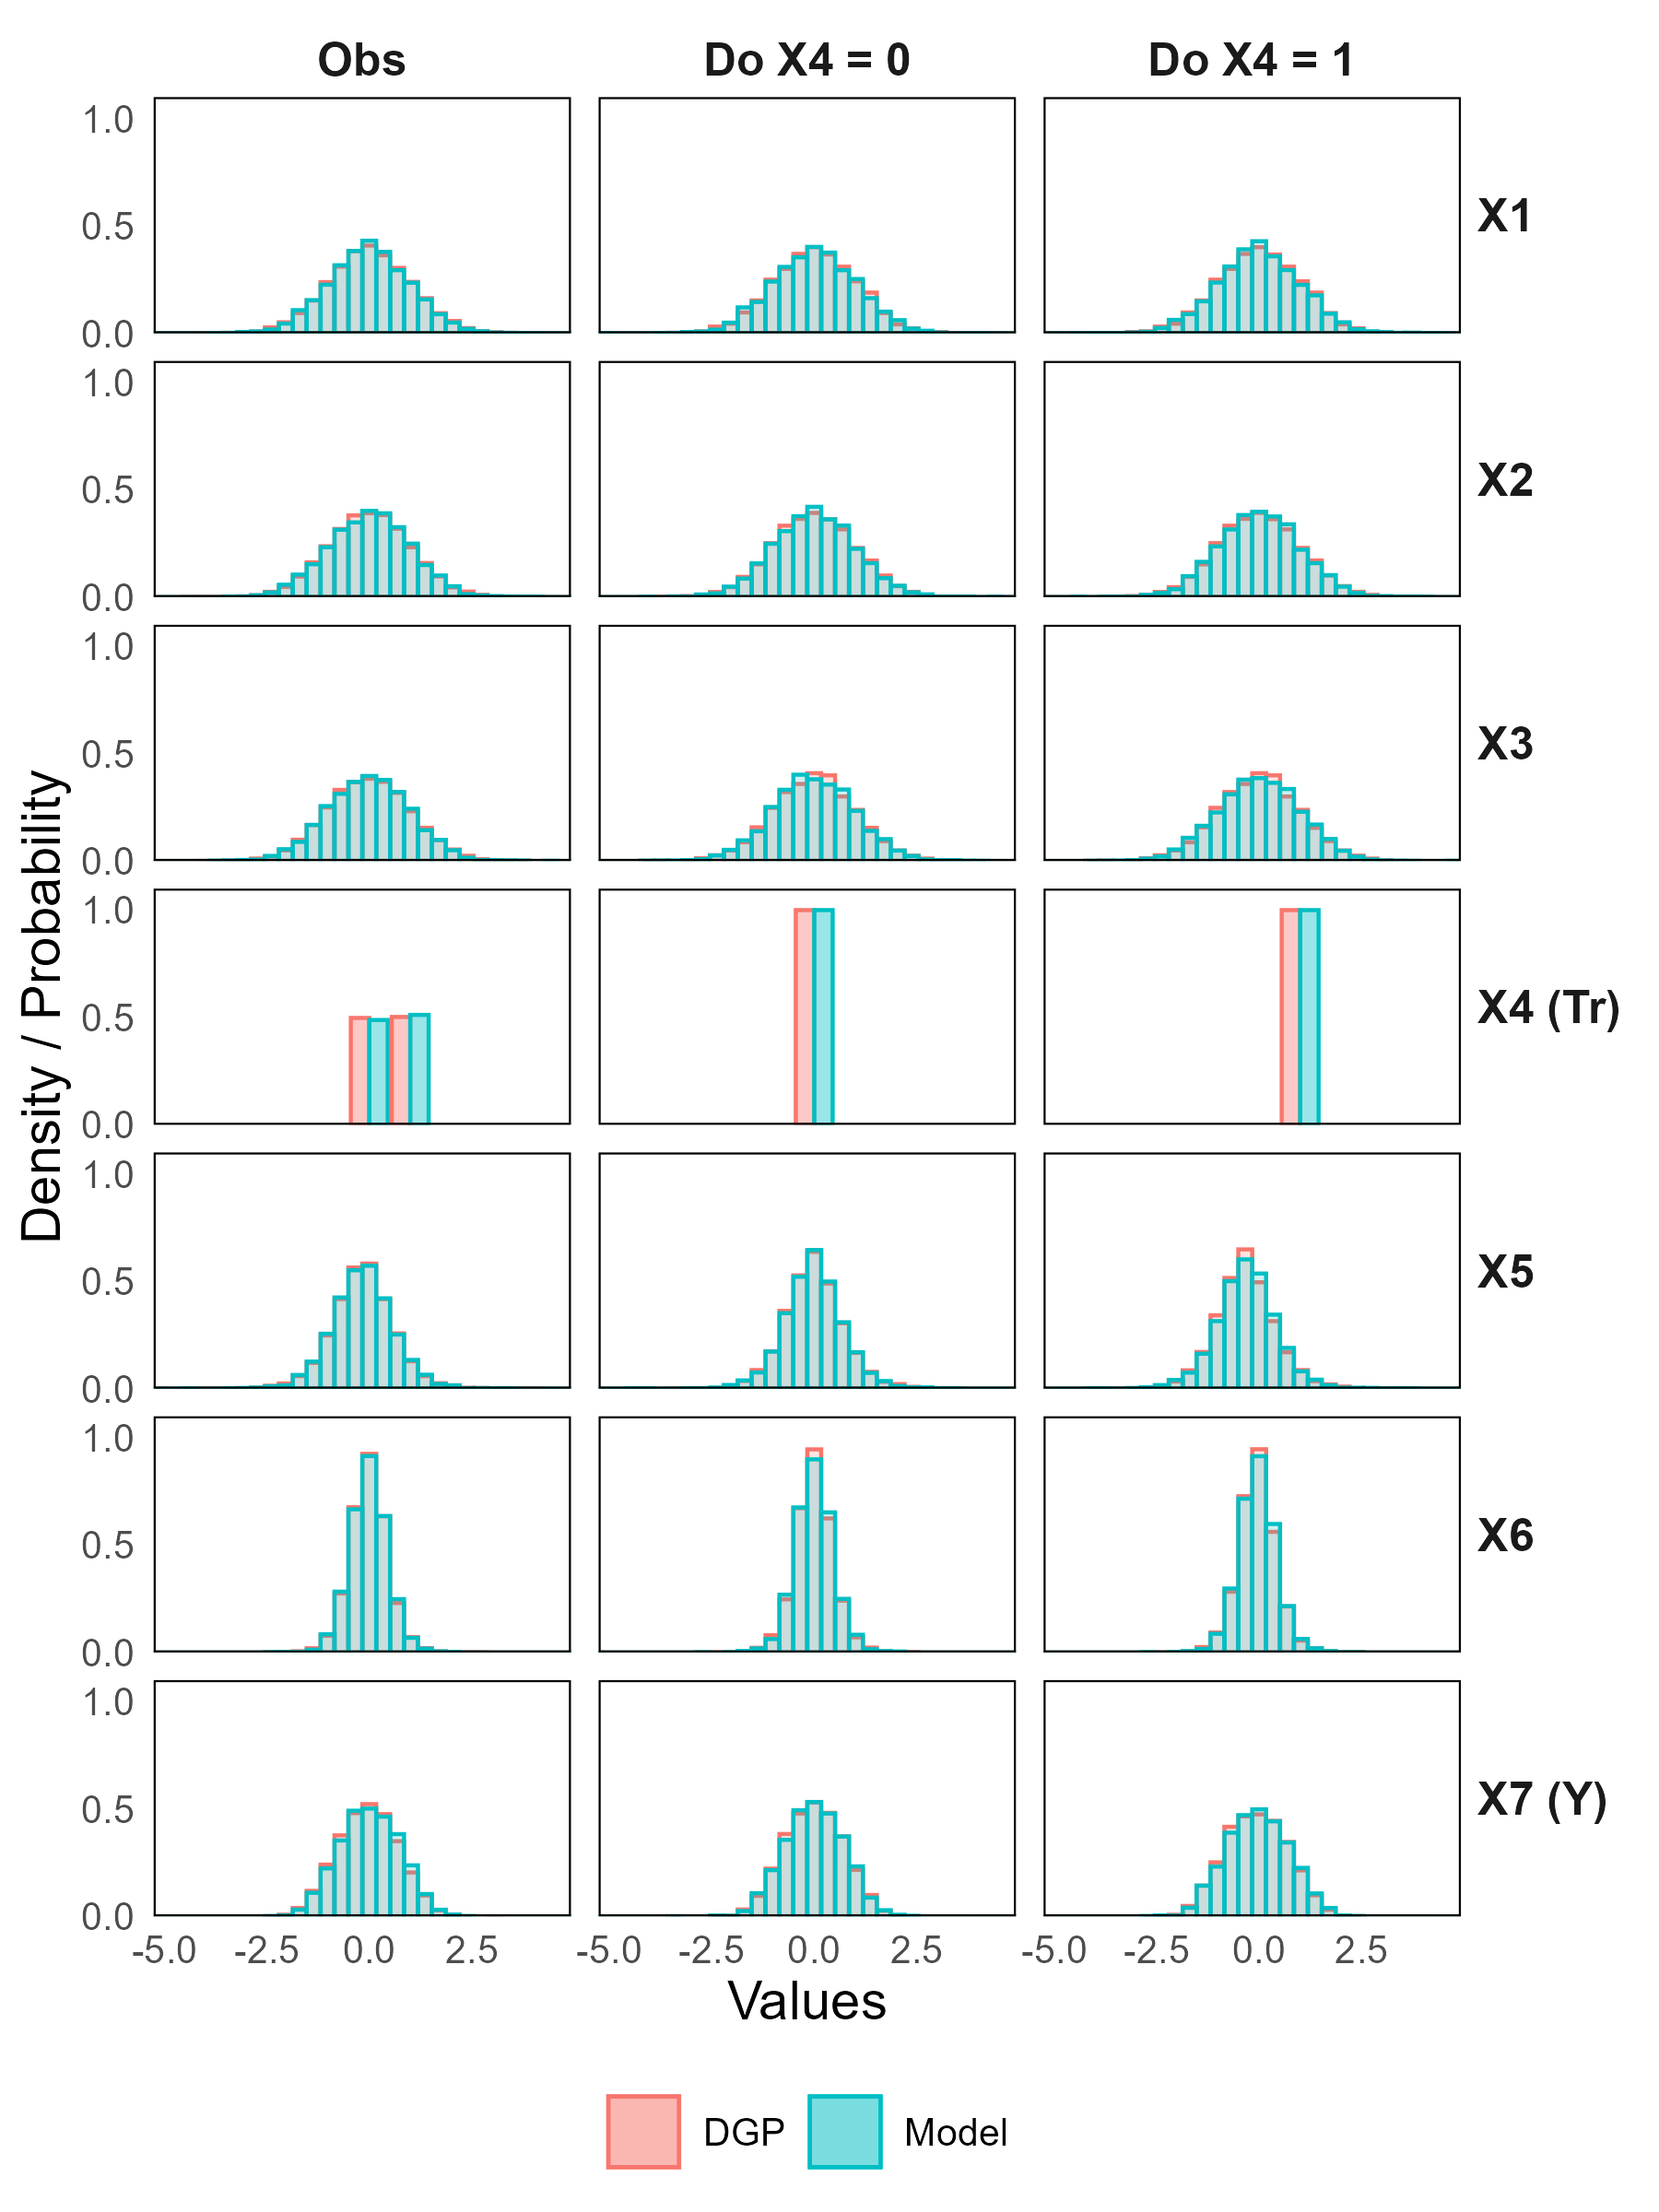
\includegraphics[width=0.45\textwidth]{img/results/rct_scenario3_sampling_distributions_vertical.png}
\caption{Marginal distributions of DGP variables and samples generated by the fitted TRAM-DAG for Scenario~(3), which includes interaction effects but no direct treatment effect. The distributions are shown as observed (Obs), under control intervention (do($X_4 = 0$)), and under treatment intervention (do($X_4 = 1$)). Left: Observational; Right: RCT setting.}
\label{fig:scenario3_sampling_distributions_vertical}
\end{figure}

\begin{figure}[htbp]
\centering
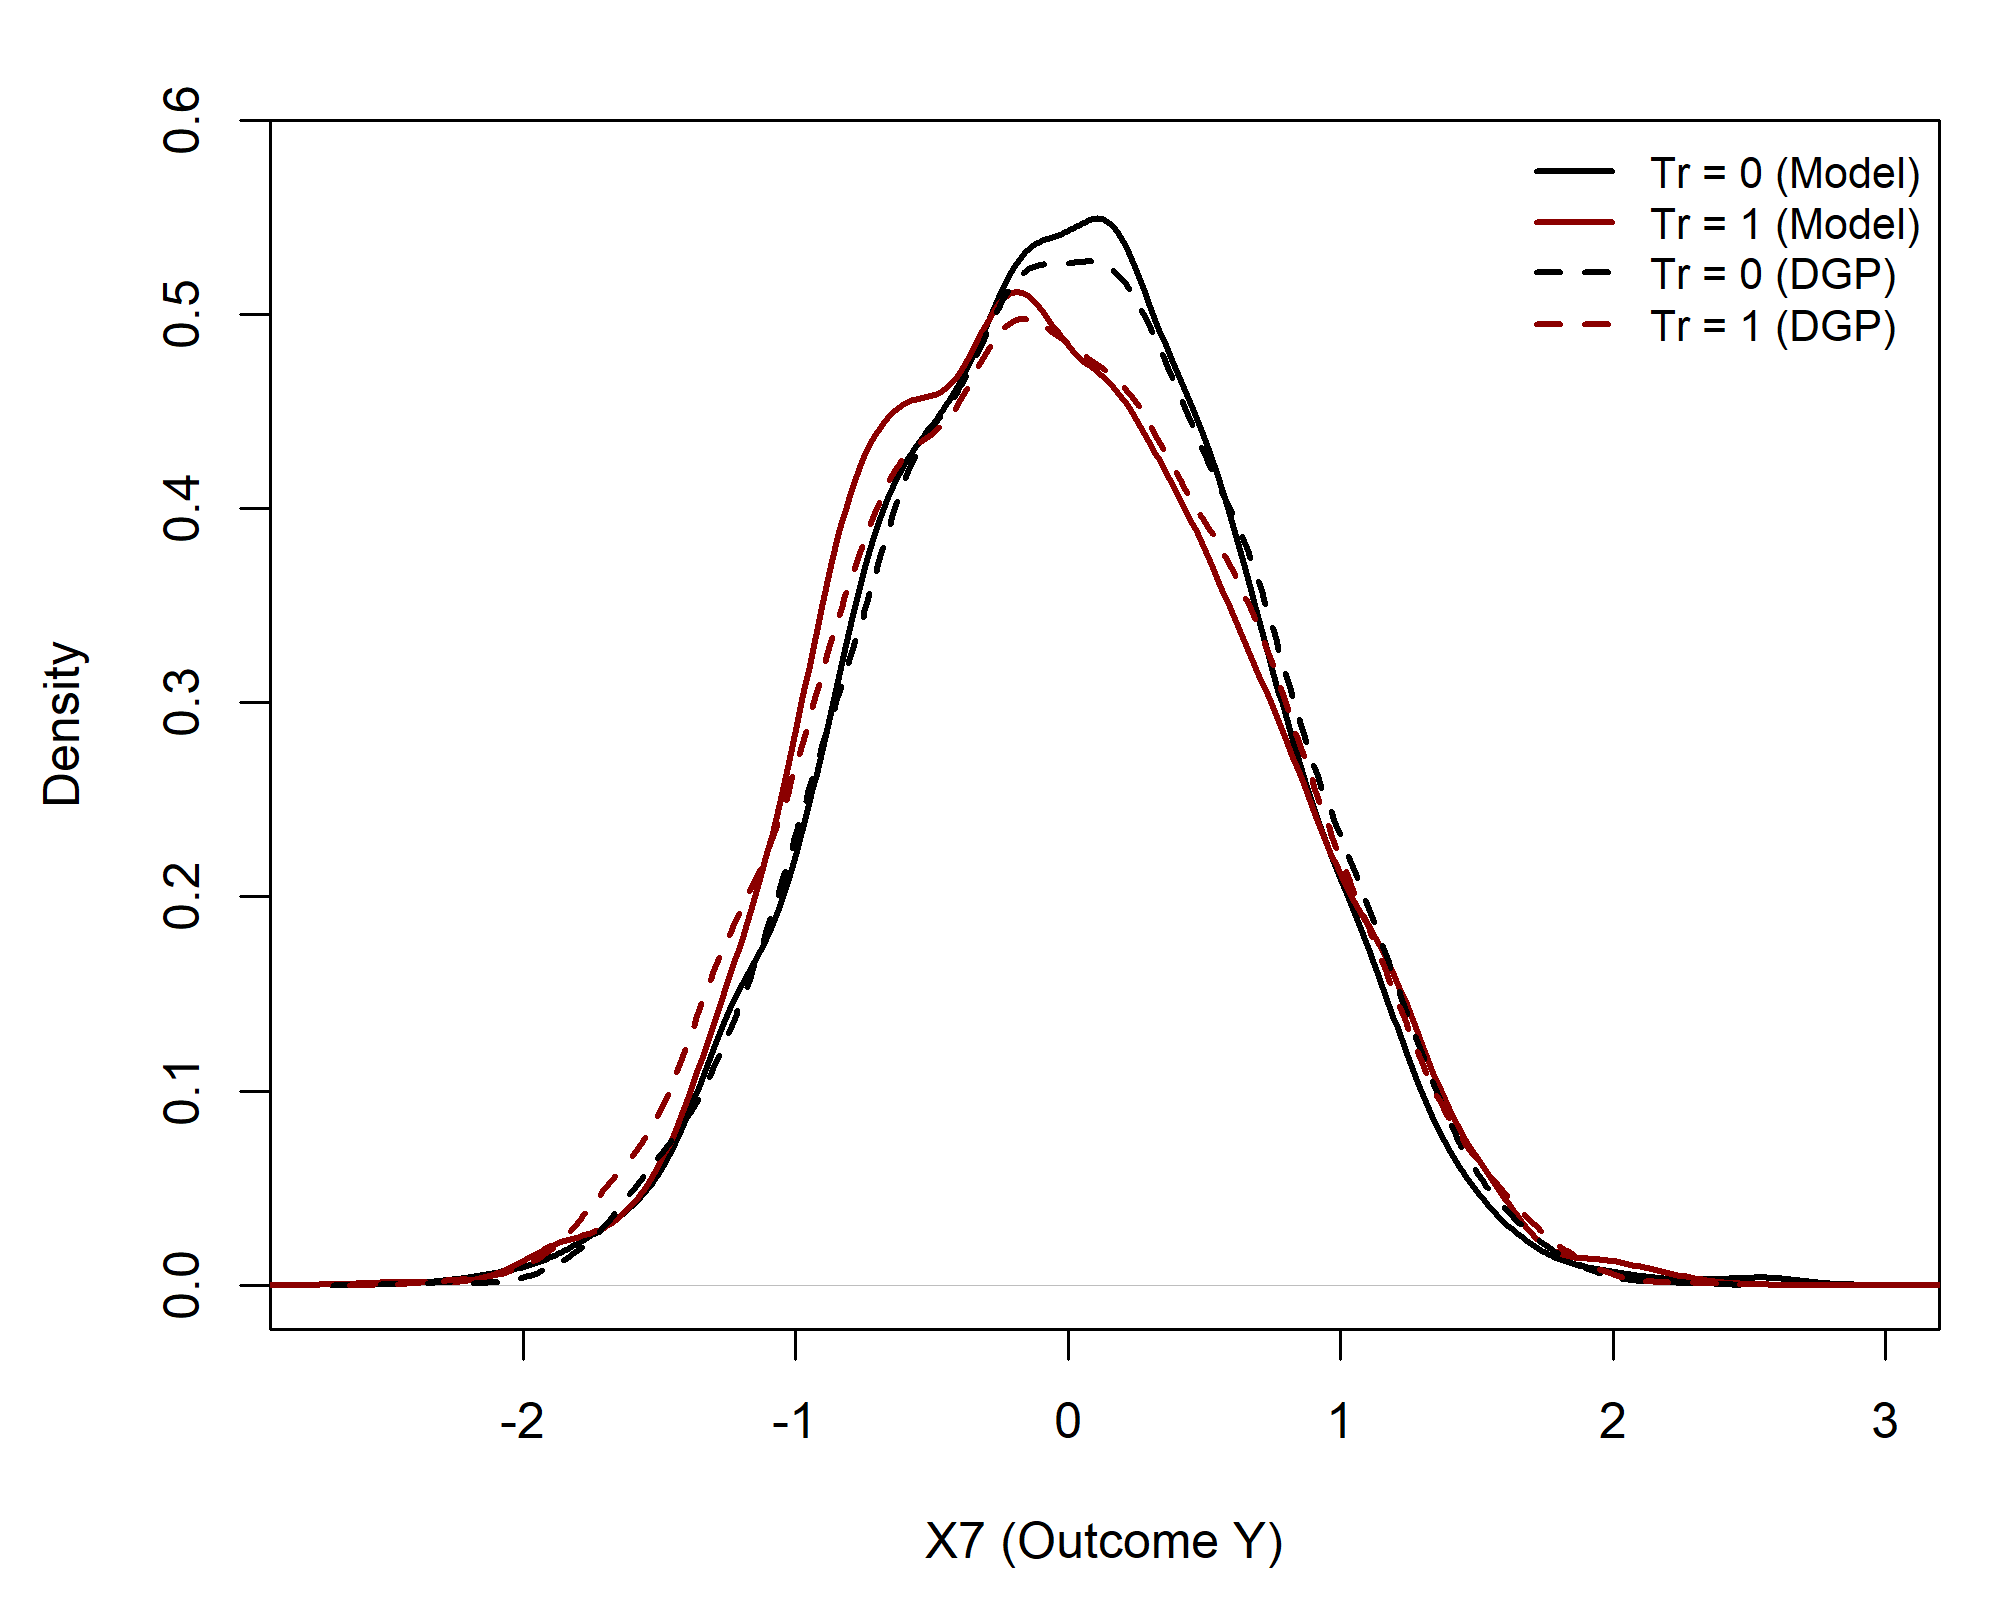
\includegraphics[width=0.45\textwidth]{img/results/observ_scenario3_X7_treatment_densities.png}
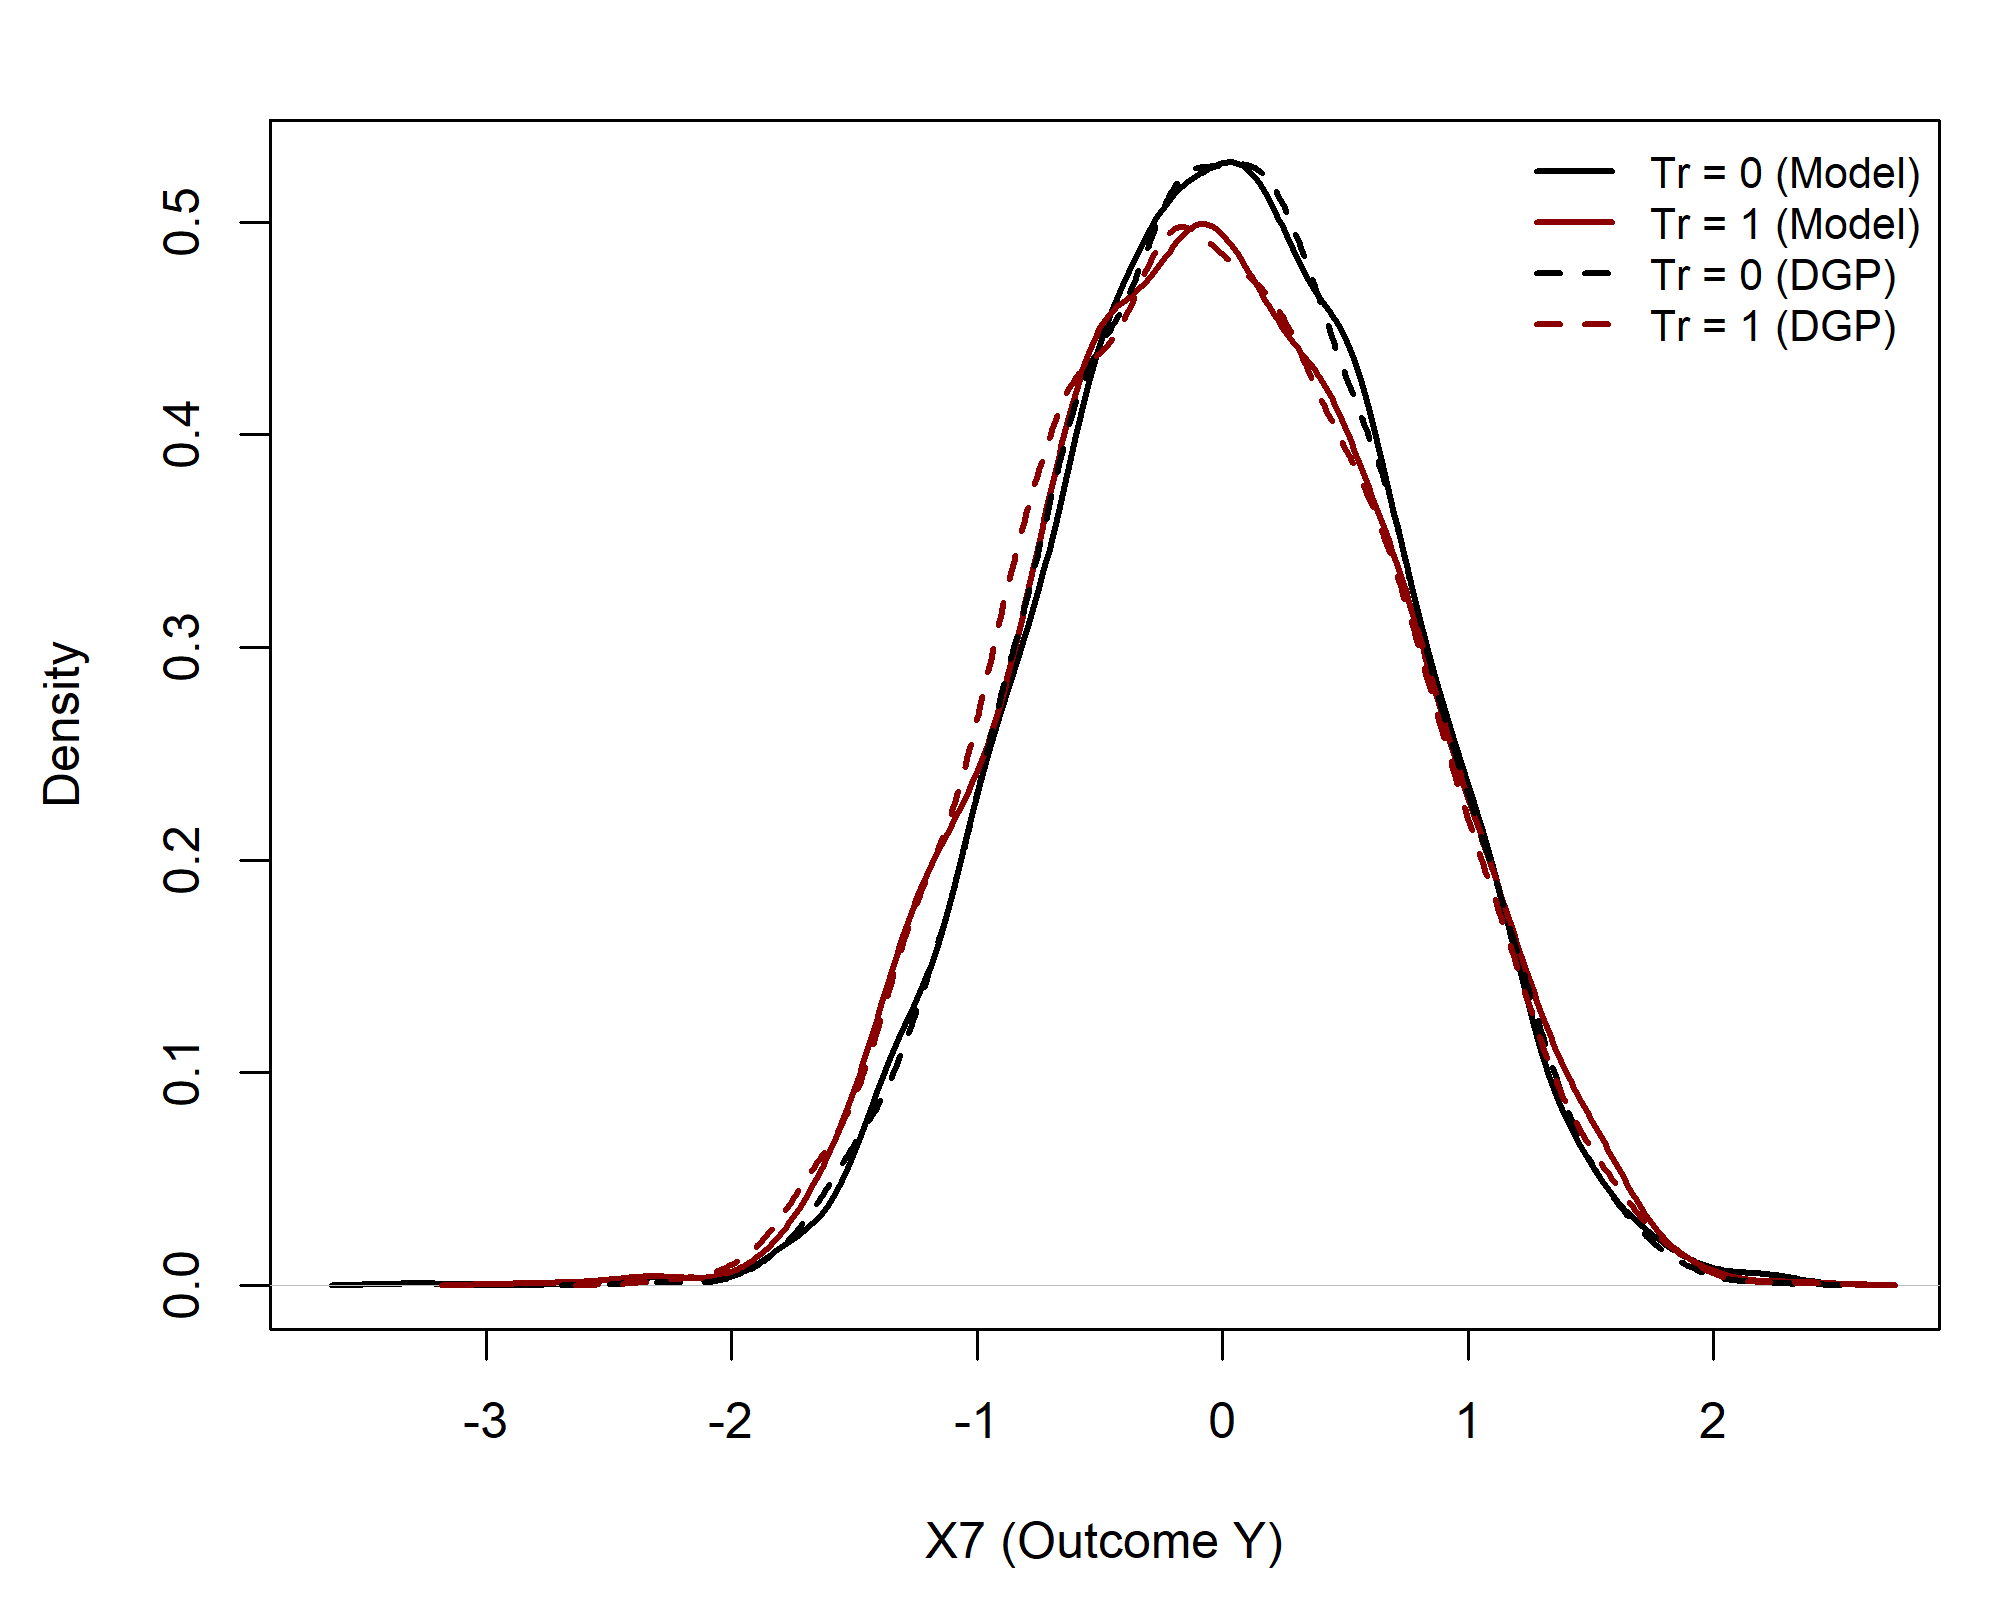
\includegraphics[width=0.45\textwidth]{img/results/rct_scenario3_X7_treatment_densities.png}
\caption{Distributions of the outcome variable ($X_7$) under treatment and control interventions for Scenario~(3), which includes interaction effects but no direct treatment effect. This plot provides a higher resolution view of the $X_7$ panels under do($X_4 = 0$) and do($X_4 = 1$) from Figure~\ref{fig:scenario3_sampling_distributions_vertical}. Left: Observational; Right: RCT setting.}
\label{fig:scenario3_outcome_distributions}
\end{figure}




\begin{figure}[htbp]
\centering
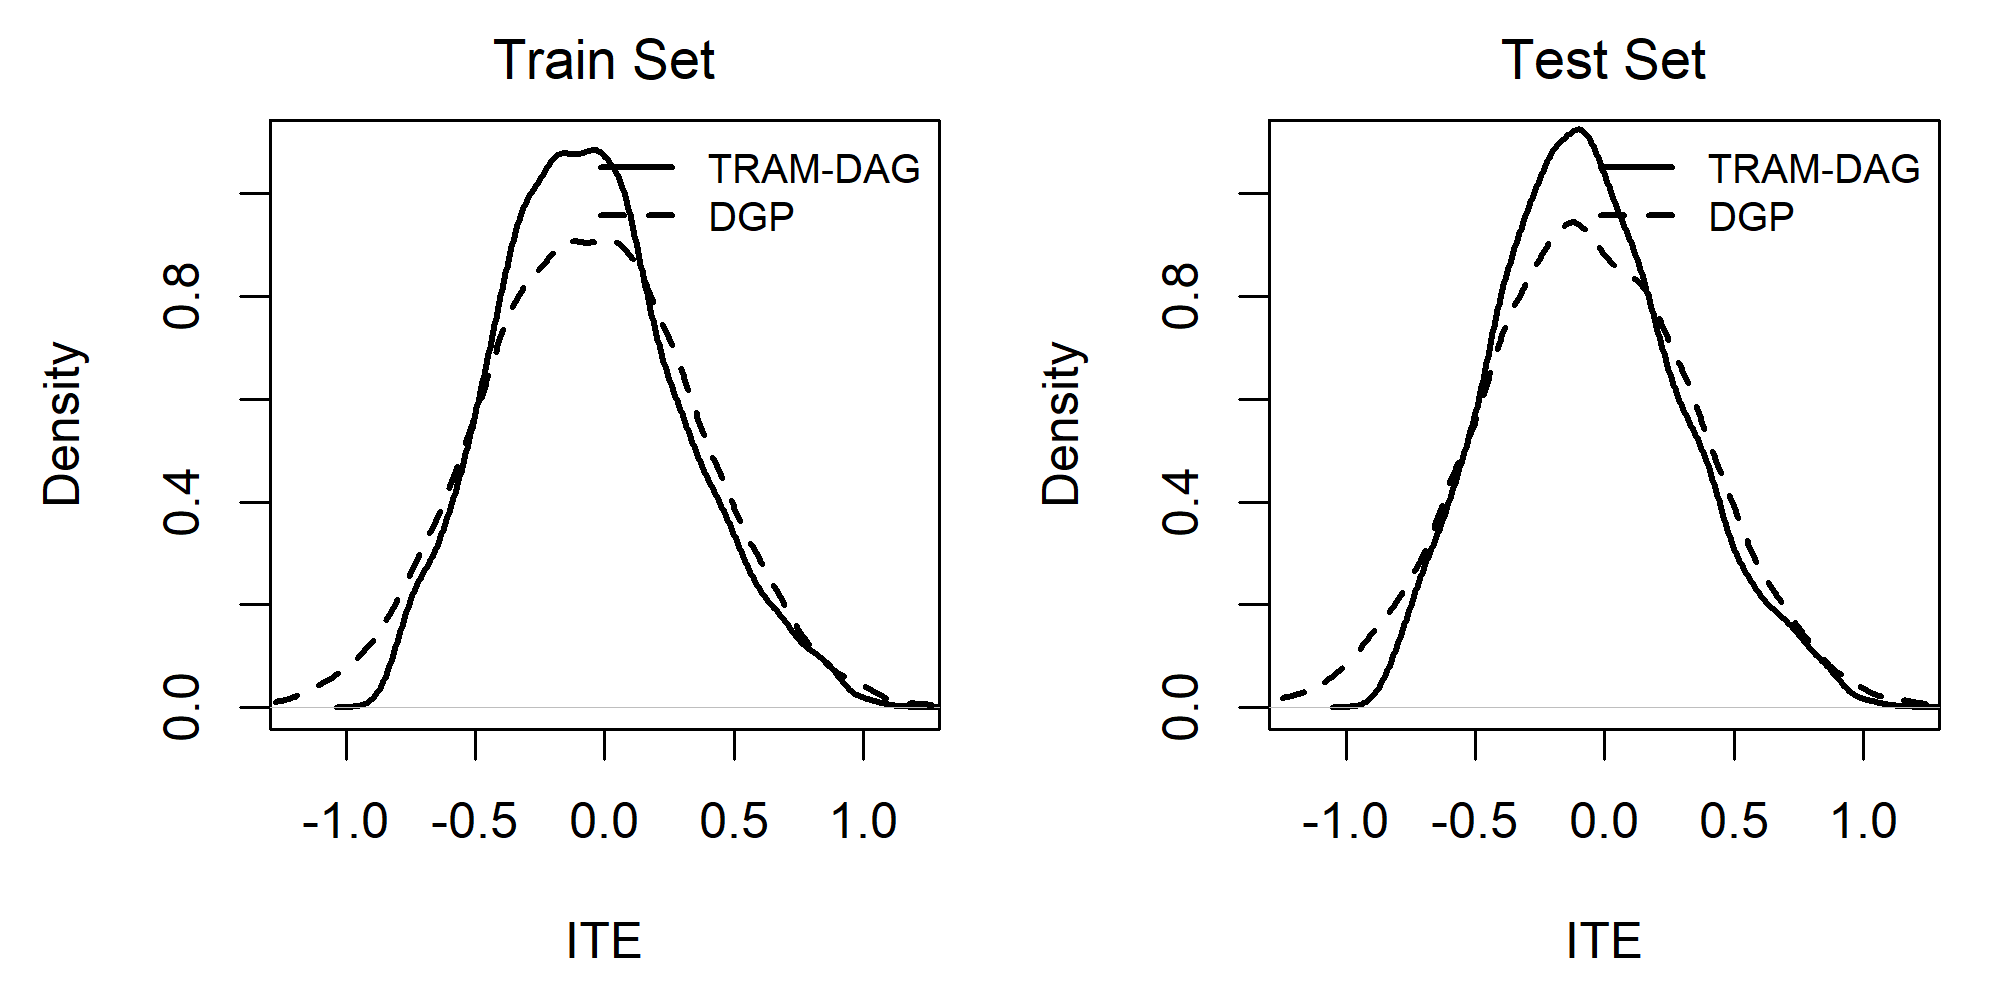
\includegraphics[width=0.33\textwidth]{img/results/observ_scenario3_ITE_densities_train_test.png}
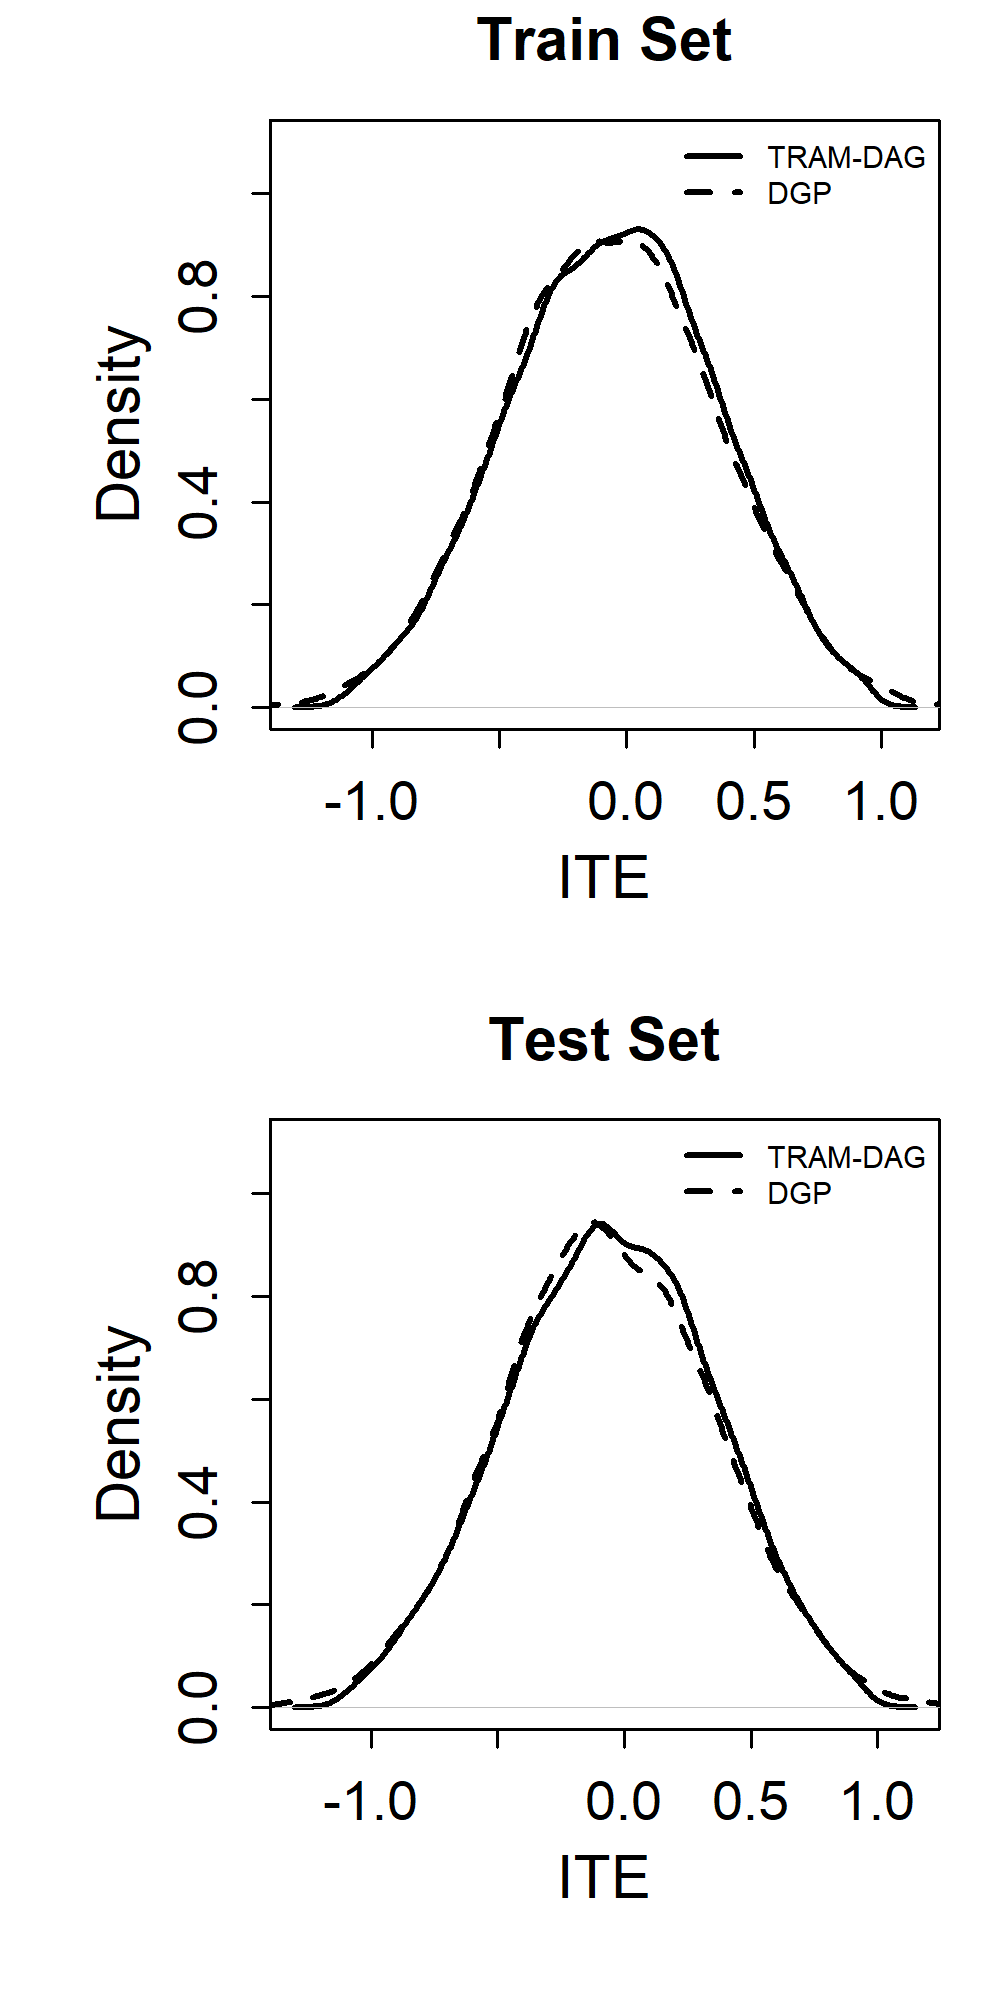
\includegraphics[width=0.33\textwidth]{img/results/rct_scenario3_ITE_densities_train_test.png}
\vspace{-17pt}
\caption{Densities of estimated ITEs compared to the true ITEs in the training and test datasets for Scenario~(3), which includes interaction effects but no direct treatment effect. Left: Observational; Right: RCT setting.}
\label{fig:scenario3_ite_densities_train_test}
\end{figure}






\begin{figure}[htbp]
\centering
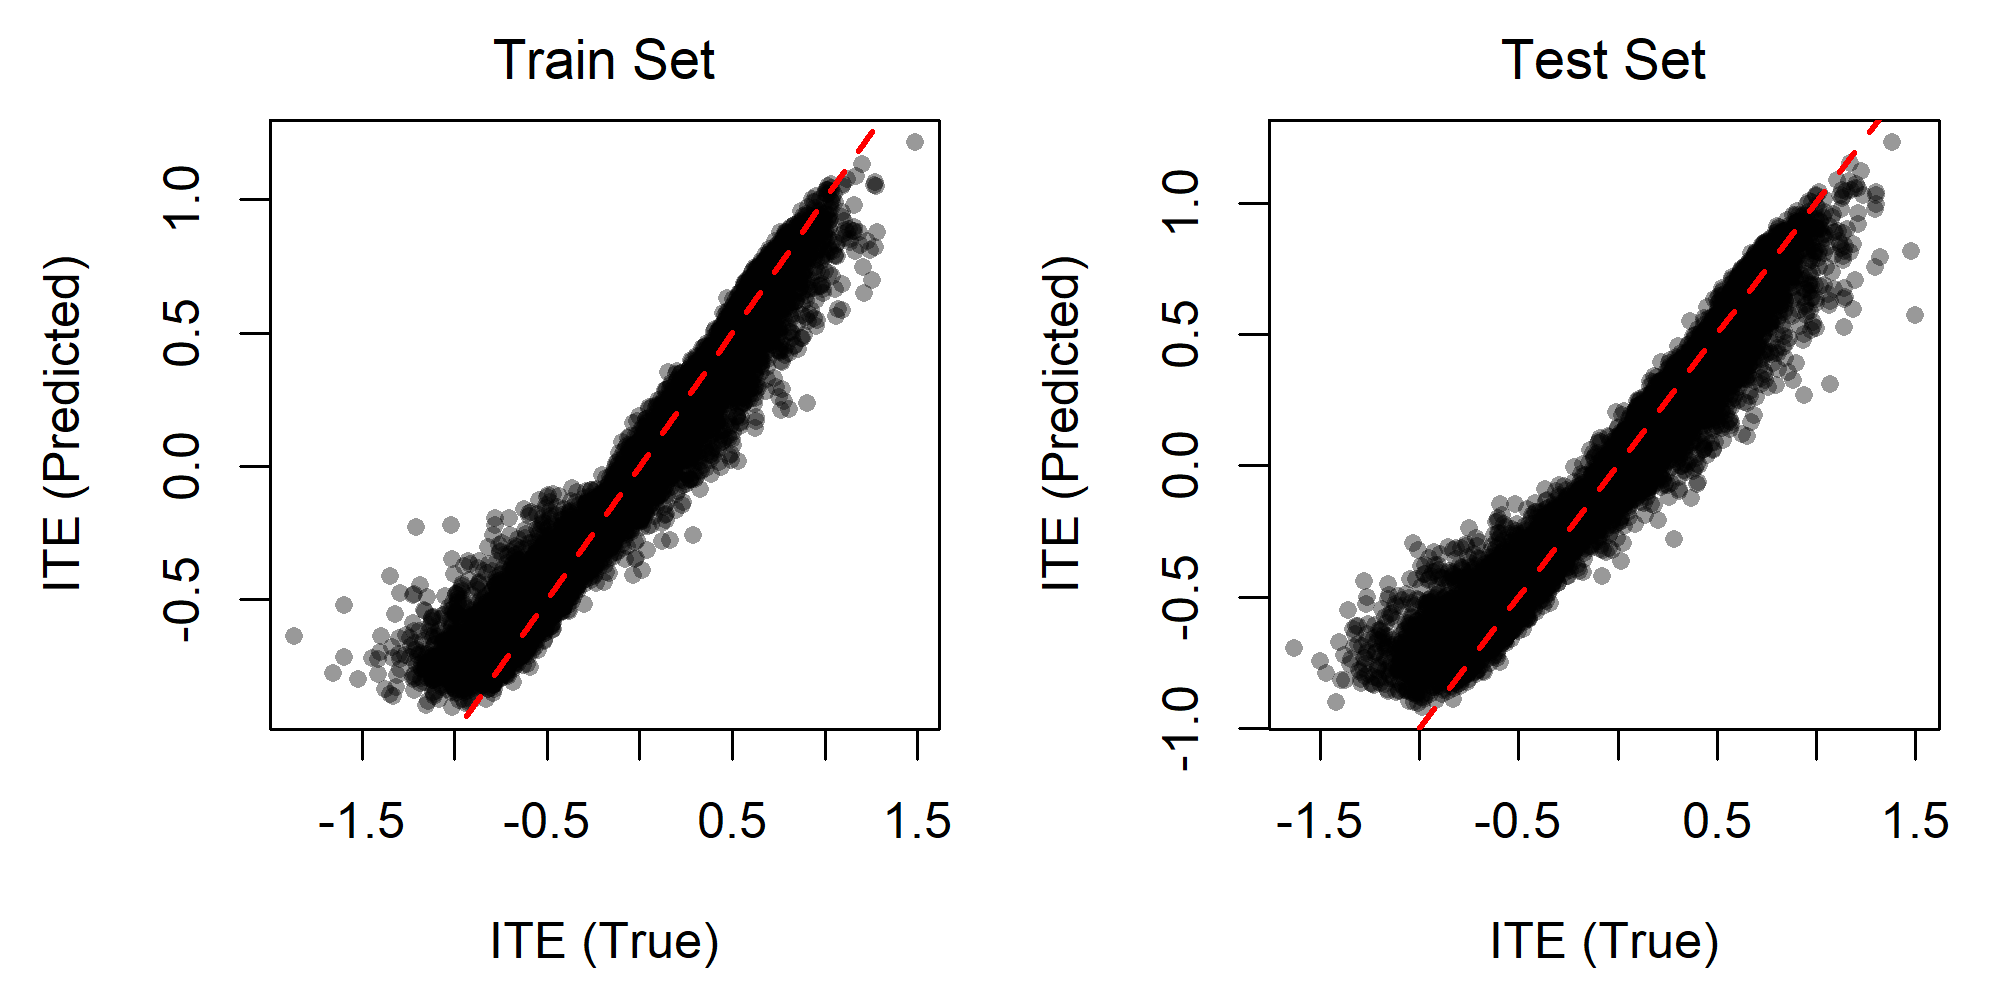
\includegraphics[width=0.33\textwidth]{img/results/observ_scenario3_ITE_scatter_train_test.png}
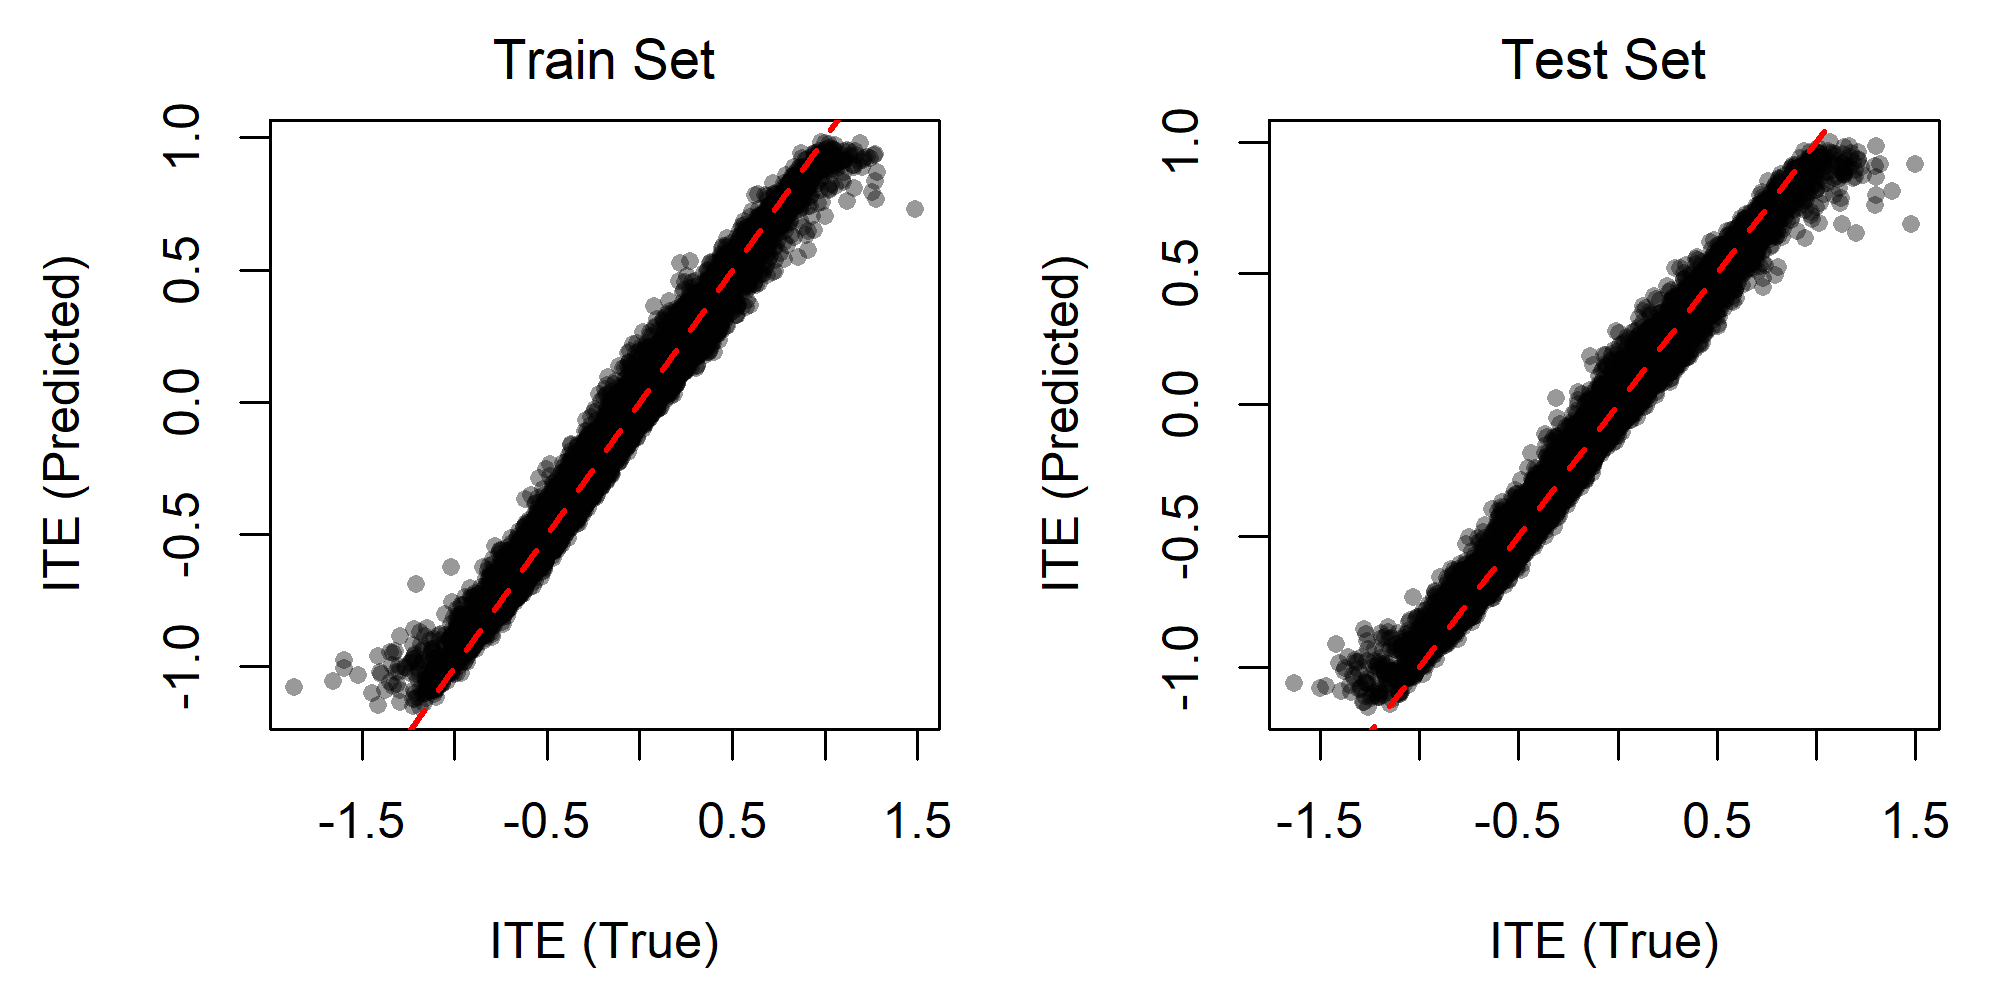
\includegraphics[width=0.33\textwidth]{img/results/rct_scenario3_ITE_scatter_train_test.png}
\vspace{-17pt}
\caption{Scatterplots of estimated ITEs compared to the true ITEs in the training and test datasets for Scenario~(3), which includes interaction effects but no direct treatment effect. Left: Observational; Right: RCT setting.}
\label{fig:scenario3_ite_scatter_train_test}
\end{figure}




\begin{figure}[htbp]
\centering
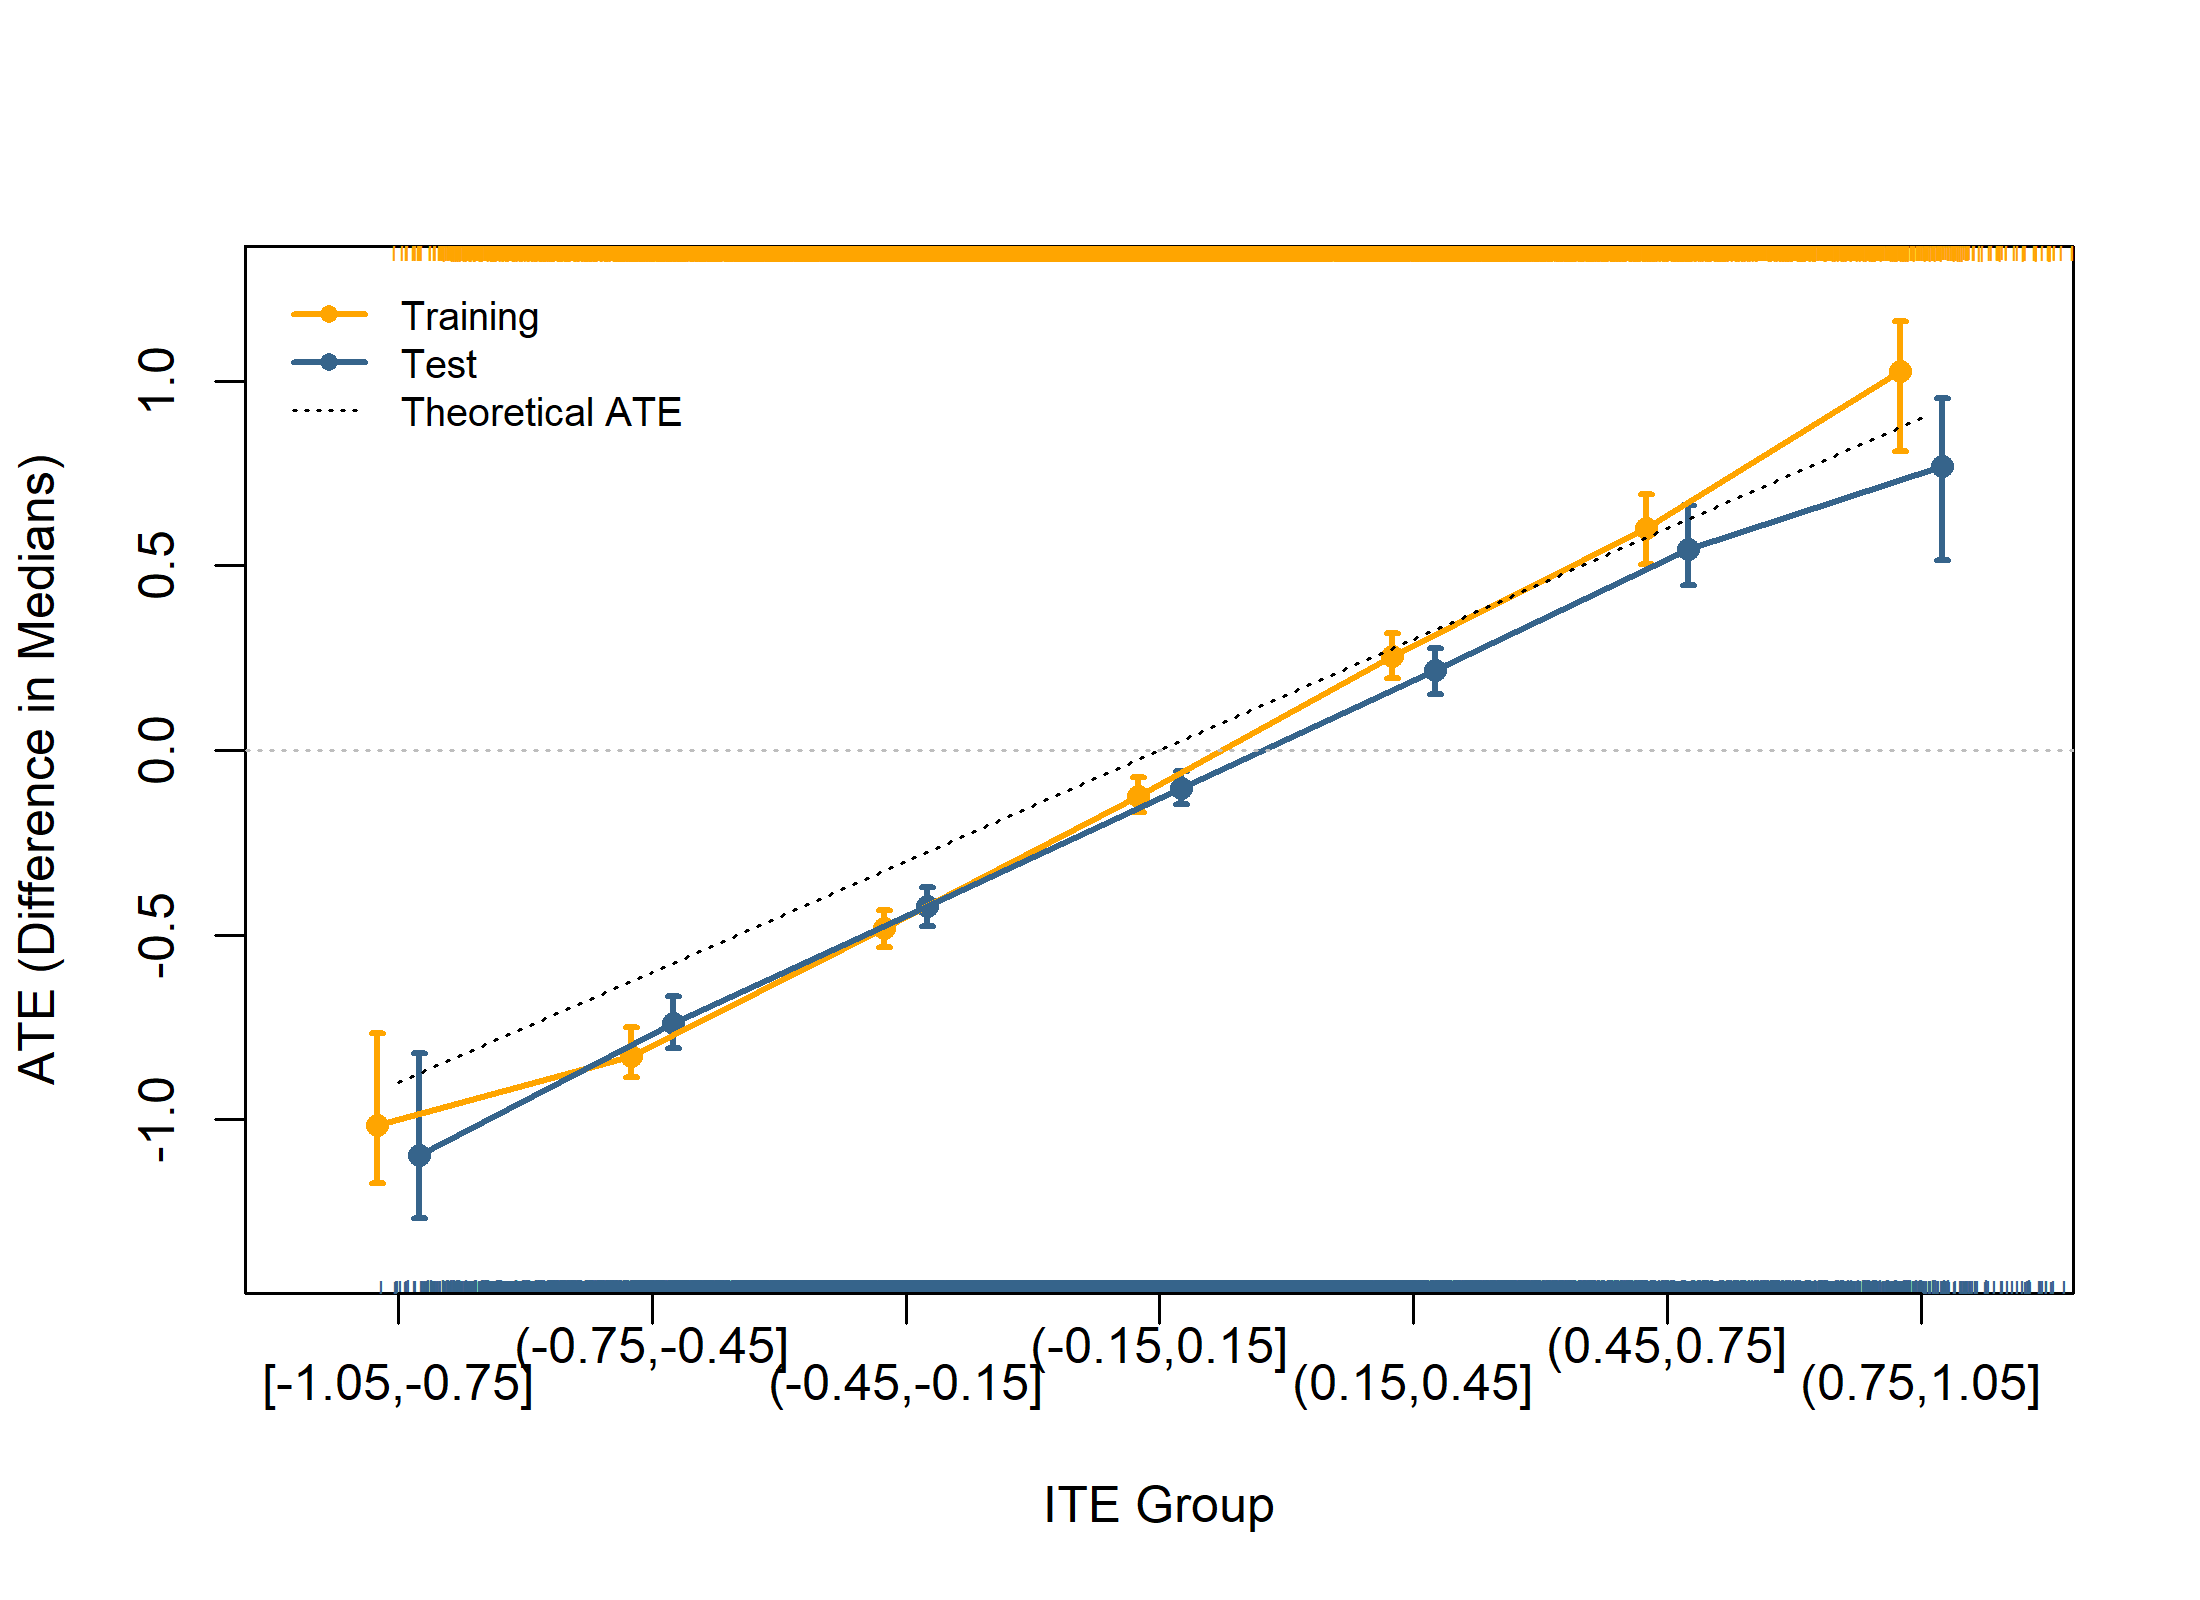
\includegraphics[width=0.8\textwidth]{img/results/observ_scenario3_ITE_ATE.png}
\vspace{-15pt}
\caption{ITE-ATE plot for Scenario~(3) in the observational setting, which includes interaction effects but no direct treatment effect. Individuals are grouped into bins based on the estimated ITE, and within each bin the ATE is computed as the difference in medians of the observed outcomes under treatment and control. 95\% bootstrap confidence intervals reflect the uncertainty.}
\label{fig:observ_scenario3_ite_ATE}
\end{figure}


\begin{figure}[htbp]
\centering
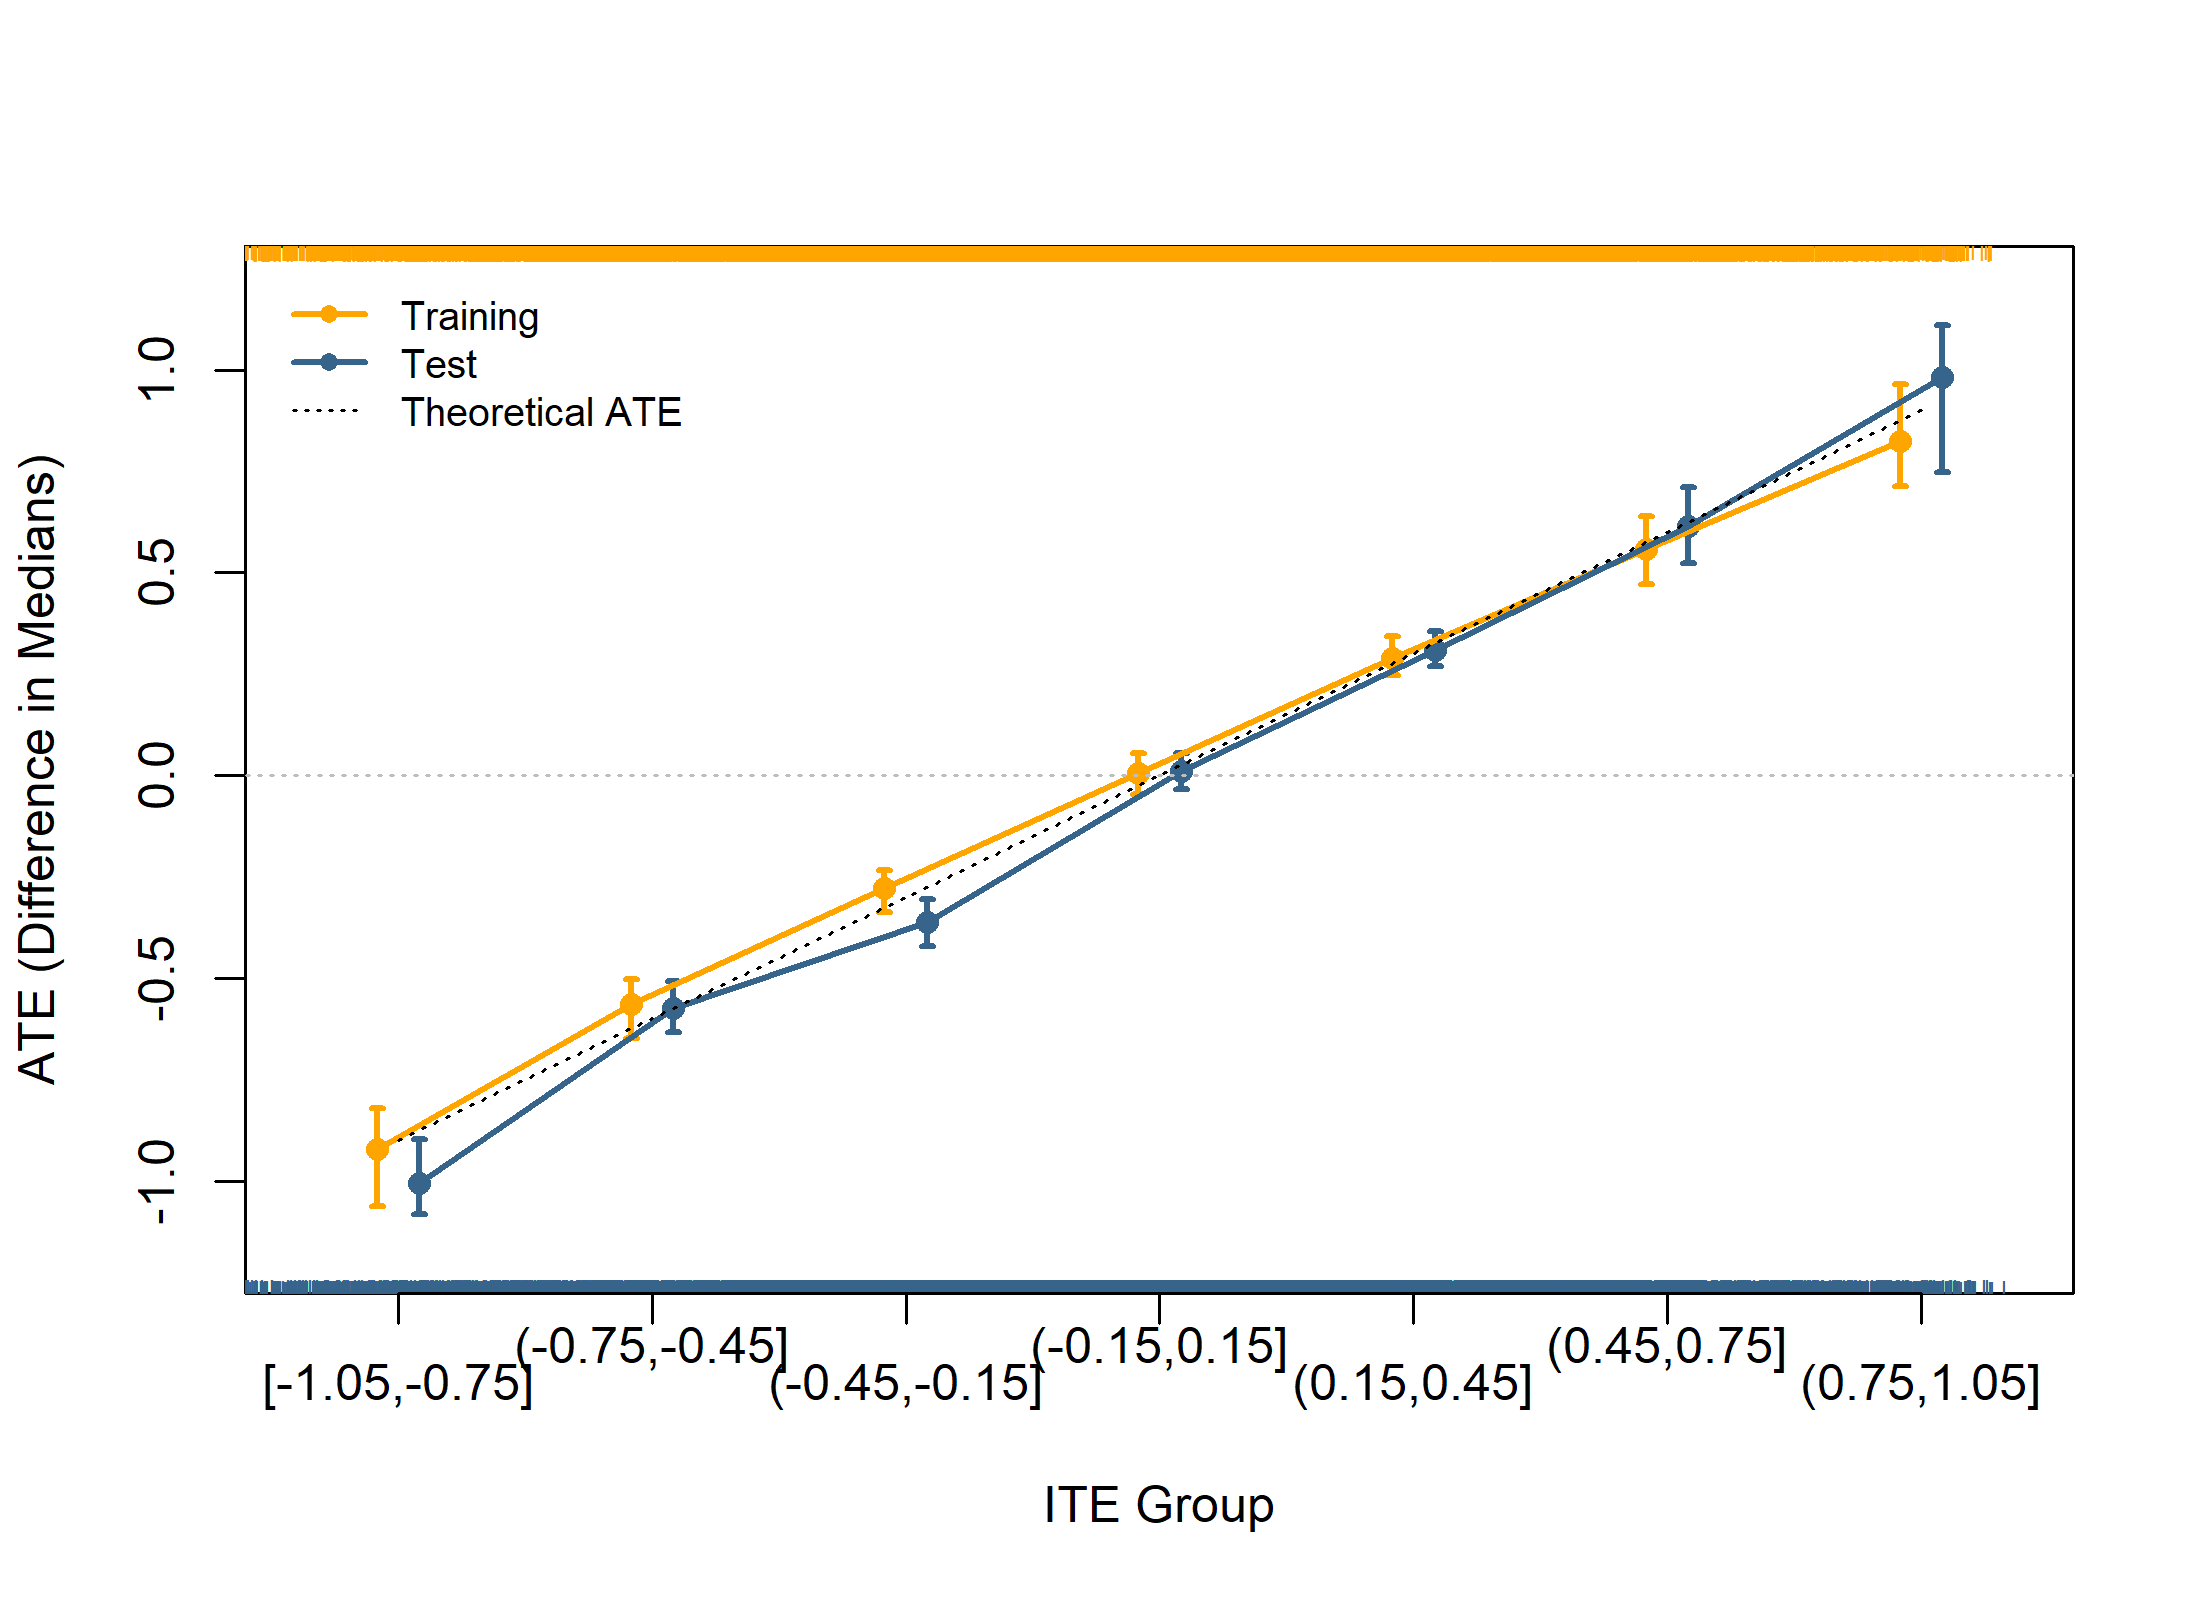
\includegraphics[width=0.8\textwidth]{img/results/rct_scenario3_ITE_ATE.png}
\vspace{-15pt}
\caption{ITE-ATE plot for Scenario~(3) in the RCT setting, which includes interaction effects but no direct treatment effect. Individuals are grouped into bins based on the estimated ITE, and within each bin the ATE is computed as the difference in medians of the observed outcomes under treatment and control. 95\% bootstrap confidence intervals reflect the uncertainty.}
\label{fig:rct_scenario3_ite_ATE}
\end{figure}







%  --> the following will be used in Experiment 4 (methods)
% http://www.mit.edu/~vchern/papers/ch_iqr_ema.pdf estimate the quantile treatment effect (heterogeneous) with instrumental variables, it looks very similar to the TRAM-DAG approach: *This interpretation makes quantile analysis an interesting tool for describing and learning the structure of heterogeneous treatment effects and controlling for unobserved heterogeneity."

% https://www.rfberlin.com/wp-content/uploads/2024/12/24030.pdf good book/paper about instrumental variables, also talks about potential outcomes (but i should maybe not go too much into detial)

% - maybe include somewhere the discussion about the difference between discrimination and claibraion:
% https://bavodc.github.io/websiteCalibrationCurves/articles/CalibrationCurves.html




% An example could be the psychological condition of a patient which might also affect how the treatment works, this is not a confounder but an effect modifier, and i would assume that this variable is rarely recorede or measured.



% enforce that starts after all floats have been displayed
\FloatBarrier


\section{Discussion} \label{sec:disc_experiment4}


We analyzed ITE estimation under an observational setting (confounded) and under an RCT setting (randomized treatment allocation) in three different scenarios: direct and interaction treatment effect, only direct but no interaction effect, and no direct but with interaction effect. The TRAM-DAG could successfully estimate the ITE in Scenario 1 and Scenario 3 where interaction effects were present. There was no notable difference between the observational and RCT settings. Scatterplots of estimated ITEs vs. true ITEs showed good prediction accuracy (see Figures \ref{fig:scenario1_ite_scatter_train_test} and \ref{fig:scenario3_ite_scatter_train_test}). Also the ATE based on the mean of estimated ITEs was close to the ATE based on true ITEs in both scenarios (see Tables \ref{tab:scenario1_ate_comparison} and \ref{tab:scenario3_ate_comparison}). These results highlight TRAM-DAG's ability to compute counterfactuals for mediators and to estimate individualized treatment effects even in relatively complex DAG structures.



In Scenario 2, where no interaction effects were present, ITE estimation was poor. This aligns with our discovery in Experiment 3 that when true heterogeneity is weak, models tended to estimate too large heterogeneity, as e.g. shown in Figure \ref{fig:small_interaction_tuned_rf_tlearner} with the T-learner tuned random forest.

\medskip

What might be surprising in Scenario 2 is the presence of heterogeneity (true ITEs), despite the absence of explicitly specified interaction terms in the data-generating process. As shown in Figure~\ref{fig:scenario2_ite_distribution_dgp}, one might have expected the ITEs to be constant across individuals -- equal to the ATE -- given the model's additivity on the log-odds scale. However, as described by \citet{hoogland2021}, such heterogeneity arises because a constant treatment effect on the log-odds scale does not translate into a constant effect on a different scale, such as the probability scale. This phenomenon results from the nonlinearity of the inverse-link function (e.g., $\text{logit}^{-1}$), which transforms additive effects in the linear predictor into non-additive effects on the outcome scale. As the authors point out, the same shift induced by the treatment on the log-odds scale leads to different absolute risk reductions depending on the outcome risk under the control treatment. In other words, even with a homogeneous effect on the linear predictor, variation in covariates $\mathbf{X}$ leads to different treatment effects on the probability scale.

This would not have occurred under a linear model where the transformation function $h$ is the identity. In that case, the ITE would simplify as follows:

\begin{equation}
\text{ITE} = \mathbb{E}[Y(1)] - \mathbb{E}[Y(0)] = (\beta_0 + \beta_t + \boldsymbol{\beta}_x^\top \mathbf{X} + \epsilon) - (\beta_0 + \boldsymbol{\beta}_x^\top \mathbf{X} + \epsilon) = \beta_t
\end{equation}

Here, the ITE is constant and equal to the treatment coefficient, independent of the covariates or the noise term, which cancels out.

In contrast, under a nonlinear model, such as the logistic transformation model with a nonlinear intercept function used in this experiment, the ITE becomes:

\begin{equation}
\text{ITE} = \mathbb{E}[h^{-1}(Z + \beta_t + \boldsymbol{\beta}_x^\top \mathbf{X})] - \mathbb{E}[h^{-1}(Z + \boldsymbol{\beta}_x^\top \mathbf{X})]
\end{equation}

Since $h^{-1}$ is nonlinear, the difference depends on the covariate profile $\mathbf{X}$ and on the noise term $Z$, even though the treatment effect $\beta_t$ is additive in the linear predictor, i.e., on the log-odds scale. It may therefore be worth thinking about whether analyzing the ITE on a scale where the effect is constant offers any advantages.

\medskip


Maybe also related to this phenomenon, although not directly in the context of ITEs, is the concept of noncollapsibility, as discussed by \citet{dandl2025}. Noncollapsibility refers to the case when the treatment effect estimated from a marginal model (i.e., without covariates) does not correspond to the marginal effect that is obtained by averaging conditional treatment effects (i.e., adjusted for prognostic covariates) over the covariate distribution \citet{aalen2015}. Hence, treatment effects from two conditional models that use different sets of covariates for adjustment are not directly comparable if the model is noncollapsible. \citet{dandl2025} proposed a solution based on nonparanormal models \citep{liu2009, klein2022} to estimate a marginal treatment effect, while maintaining comparability (unaffected by covariates) and gaining from increased precision by adjusting for prognostic factors. Whether and how such an approach could be applied to ITE estimation is not explored further in this thesis.


% Maybe also related to this phenomenon, although not in the context of ITEs, might be the concept of non-collapsibility, as discussed by \citet{dandl2025}. Non-collapsibility refers to the case when the treatment effect from a marginal model does not correspond to the marginal effect that is obtained from a conditional treatment effect (i.e. adjusted for prognostic covariates) by averaging over the prognostic variables. Hence, treatment effects from two conditional models that used different sets of covariate for adjustments are not comparable if a model is non-collapsible. The authors proposed a solution based on nonparanomrmal models (\citealp{{liu2009}; \citealp{klein2022}) to estimate a marginal treatment effect, while maintaining comparability (unaffected by covariates) and gaining from increased precision by adjusting for prognostic factors. However, if and how this would translate to ITE estimation goes beyond the scope of this thesis.

% What might be surprising is that in Scenario 2 where we dont have explicitly included interaction terms in the data generating process, there is still some heterogeneity in the treatment effect, as shown in Figure \ref{fig:scenario2_ite_distribution_dgp}. One might expect that the ITE is constant across all individuals in such a case, and equal to the ATE. 
% 
% \citep{hoogland2021} chapter 4.1 well described this phenomenon of non-additivity leaving the log-odds scale.
% % the problem with non-additivity is perffectly described in Hoogland "A tutorial on individualized treatment effect prediction from randomized trials with a binary endpoint
% 
% However since we used a non linear transformatino function as intercept in the data generating process (as would likely be the case in a real world setting), the treatment effect is not constant across all individuals (which should correspond to the ATE). When a linear transformation function would be applied (as for example a linear regression is specified, where the latent noise distribution would be the standard normal and the transformation function would be linear) then the noise term cancels out when calculating the ITE, leading to a constant ITE when no interactions are present: $\text{ITE} = \text{E}[Y(1)] -\text{E}[Y(0)] = (\beta_0 + \beta_t 1 + \beta_x X + \epsilon) - (\beta_0 + \beta_t 0 + \beta_x X + \epsilon) = \beta_t$.
% 
% In a model with nonlinear transformation, as in this experiment, the noise term does not cancel out anymore leading to different ITEs for patients with different characteristics.
% 
% \begin{equation}
% \text{ITE} = \text{E}[Y(1) - Y(0)] = \text{E}[h^{-1}(Z + \beta_t 1 + \beta_x X)] - \text{E}[h^{-1}(Z + \beta_t 0 + \beta_x X)] 
% \end{equation}
% 
% where $h$ is the nonlinear transformation function, $Z$ is the latent noise term, $\beta_t$ is the direct treatment effect and $\beta_x$ are the coefficients of the covariates. The state of the covariates $X$ alters the position on the transformation function and thereby affects the difference between the two terms. If the transformation was fixed to be linear, the difference would be constant independent of the state of the covariates $X$. 

% (This also has to do with non-collapsibility as discussed by susanne and torsten , also check Beates Mail 21.06.2025, and chatgpt discussion)



% cite susanne and torsten paper: https://arxiv.org/abs/2503.01657




